\documentclass[titlepage,openright,twoside,a4paper,12pt]{book}

\usepackage[russian,english]{babel}
\usepackage[pdftex,final]{graphicx}
\usepackage[listings,theorems,skins,breakable]{tcolorbox}
\usepackage[labelfont=bf]{caption}
\usepackage{tikz}
\usetikzlibrary{shapes.geometric}
\usetikzlibrary{arrows.meta}
\usepackage{epigraph}
\usepackage[explicit]{titlesec}
\usepackage{rotating}
\usepackage{multirow}
\usepackage{amsmath}
\usepackage{amsfonts}
\usepackage{eurosym}
\usepackage{bbding}
\usepackage{pifont}
\usepackage{tabularx}
\usepackage{paralist}
\usepackage{enumitem}
\usepackage[utf8]{inputenc}  
\usepackage[T1]{fontenc}
\usepackage{setspace}
\usepackage{xcolor}
\usepackage{xspace}
\usepackage{parskip}
\usepackage{changepage}

% %enlaces
\usepackage[hidelinks]{hyperref}


% %pie de página
\usepackage{lastpage}
\usepackage{fancyhdr}
%\pagestyle{fancy}

% fix overfull \hbox
\usepackage{microtype}

%eliminar el guionado
\tolerance=1
\emergencystretch=\maxdimen
\hyphenpenalty=10000
\hbadness=10000

\renewcommand{\baselinestretch}{1.5}


% Paquetes ABD
\usepackage{lettrine} % Para primera letra grande en los capítulos
\usepackage{Zallman} % fuente de la primera letra de los capítulos
\usepackage{todonotes} % para todonotes... duh

% para definiciones
\usepackage{amsmath, amssymb, amsthm}
\newtheorem{definition}{Definition}
\let\proof\relax
\let\endproof\relax % to avoid name clashes

\usepackage[square, numbers, sort]{natbib} % citas
\usepackage{subfigure} % subfiguras

% algoritmos
\usepackage[ruled, vlined, linesnumbered]{algorithm2e}
\usepackage{algpseudocode}

\usepackage{array} % tablas
\usepackage{svg} % figuricas en svg
\usepackage{afterpage} % para la tabla grande que debe empezar en página par
\usepackage[export]{adjustbox} % Figuras alineadas a izquierda y derecha para la tabla grande de los cojones
\usepackage{datetime2}  % Fechas automáticas
\usepackage{moresize}  % Comando \HUGE
\usepackage{tocbasic}  % Estilos de la TOC
\usepackage[nottoc,notlof,notlot]{tocbibind}  % Mete la bibliografía como capítulo en la TOC, los parámetros excluyen los otros índices de aparecer también
\usepackage{float}
\def\UrlBreaks{\do\/\do-}
\usepackage{amssymb} % Para el \Checkmark
\usepackage{booktabs}
\usepackage{setspace}
% Citas y abstracts de los capítulos
\newcommand{\chapterQuote}[2]{
    \vspace{-1.5cm}
    \epigraph{#1}{#2}
}

\newcommand{\chapterAbstract}[2]{
    % Seguramente haya alguna forma de pasar sólo 1 argumento
    % y extraer automáticamente la primera letra para pasársela
    % al lettrine. Los ejemplos de cosas parecidas que he
    % encontrado son todos feísimos y usan latex oscuro, así
    % que paso, no me merece la pena el esfuerzo. Si tú, usuario
    % futuro de esta plantilla, consigues hacerlo así, cambia
    % este comando y siéntete realizado con tu vida.
    \vspace{2cm}
    \lettrine{#1}{ }#2
    \newpage
}

\makeatletter
\newcommand{\monthyeardate}{%
  \DTMenglishmonthname{\@dtm@month} \@dtm@year
}

\newcommand{\monthyearcover}{%
  \DTMenglishmonthname{\@dtm@month}, \@dtm@year
}

\newcommand*{\rom}[1]{\expandafter\@slowromancap\romannumeral #1@}

\newcommand{\romanyear}{%
    \rom{\@dtm@year}
}
\makeatother

\newcommand{\hypthesis}[1]
{
    \begin{quote}
        \textit{#1}
    \end{quote}
}

% avoid having to prepend ~ to \cite and \ref all the time
% to prevent the reference from being placed in the next line
\let\oldcite\cite
\renewcommand\cite{\nolinebreak\oldcite}

\newcommand{\tripleSty}[1]{\textit{#1}}

%formatting for code excerpts
\newcommand{\code}[1]{\texttt{#1}}

% Para que figuras grandes no se coman una pagina entera
% https://tex.stackexchange.com/questions/68516/avoid-that-figure-gets-its-own-page
\renewcommand{\floatpagefraction}{.9}

%%%%%%%%%%%%%%%%%%%%%%%%%%%%%%%%%%%%%%%%%%%%%%%%%%%%%%%
%%% A partir de aquí hacia abajo son cosas que he definido yo, se pueden borrar

% this is so the text f's in math mode don't have spacing around them
% by using {\ff}
\newcommand{\ff}{\mkern-2mu f\mkern-3mu}

%tipo de columna para las tablas
\newcolumntype{M}[1]{>{\centering\arraybackslash}m{#1}}

% shortcuts para formulas
\newcommand{\fancy}[1]{\ensuremath{\mathcal{#1}}}
\newcommand{\Eset}{\fancy{E}}
\newcommand{\Rset}{\fancy{R}}
\newcommand{\Tset}{\fancy{T}}
\newcommand{\Sset}{\fancy{C}}
\newcommand{\triple}{\ensuremath{(s, r, t)}}
\newcommand{\negtriple}{\ensuremath{(s, r, t')}}
\newcommand{\KG}{\ensuremath{\textmd{\textup{\fancy{K}\fancy{G}}}}}
\newcommand{\KGlong}{\ensuremath{(\Eset{}, \Rset{}, \Tset{})}}
\newcommand{\subKG}[2]{\ensuremath{\KG_{#1}^{#2}}}
\newcommand{\subKGdef}{\subKG{n}{n}}
\newcommand{\nearby}[2]{\Eset{}_{#1}^{#2}}
\newcommand{\kgpath}[3]{\ensuremath{path(#1, #2, #3)}}
\newcommand{\kgpathl}[3]{\ensuremath{path_{#3}(#1, #2)}}
\newcommand{\kgpathP}[3]{\ensuremath{\fancy{P}(#1, #2, #3)}}


% entornos y comandos para definiciones y cosas
\newcommand{\defin}[2]{
\begin{definition}\label{#1}{\textbf{#1:}}
#2
\end{definition}
}

\newcommand{\candfunc}[2]{
    \textbf{#1}: #2
}

\newcounter{featgroup}
\newcommand{\featgroup}[6]{
    \stepcounter{featgroup}
    \textbf{\texorpdfstring{Feature group $f_{\arabic{featgroup}}$: \textit{#1}}{Feature group f\arabic{featgroup}: #1}} Features in this group are computed as: 
    \begin{equation*}
    \begin{gathered}
        f_{\arabic{featgroup}}(#2) : \triple \mapsto #3
    \end{gathered}
    \end{equation*}
    In the example shown in Figure \ref{fig:kg-potter}, $f_{\arabic{featgroup}}($\textit{#5}$)$ applied to the $\textit{example}$ triple is #6.
}

\newcounter{scifeatcount}
\newcommand{\scifeature}[2]{
    \stepcounter{scifeatcount}
    \textbf{Feature $f_{\arabic{scifeatcount}}$: #1}. #2
}

\newcommand{\roberta}{RoBERTa}


\definecolor{tickgreen}{HTML}{009B55} 
\definecolor{crossred}{HTML}{850000} 
\newcommand{\yes}{\textcolor{tickgreen}{\textbf{\checkmark}}}
\newcommand{\no}{\textcolor{crossred}{\text{\sffamily X}}}
% Fuente
\usepackage[sc]{mathpazo}

\linespread{1.2} % Espacio entre líneas
\setlength{\parindent}{20pt} % Indentación de primera línea en párrafos

% Configurar la fuente para la primera letra de los capítulos
\renewcommand{\LettrineFontHook}{\Zallmanfamily}

% Estilo para las citas al principio de los capítulos
\epigraphsize{\small\itshape}
\setlength{\epigraphwidth}{.6\textwidth}
\renewcommand{\textflush}{flushepinormal}
\setlength\epigraphrule{0pt}

% Tamaños y estilos de elementos en la TOC
\DeclareTOCStyleEntry[
    linefill=\bfseries\TOCLineLeaderFill,
    beforeskip=12pt,
    entrynumberformat=\chapterprefixintoc,
    entryformat=\chaptertocformat,
    pagenumberformat=\chaptertocformat,
    dynnumwidth
]{tocline}{chapter}

\DeclareTOCStyleEntry[
    % linefill=\bfseries\TOCLineLeaderFill,
    beforeskip=30pt,
    entrynumberformat=\chapterprefixintoc,
    entryformat=\parttocformat,
    pagenumberformat=\partpagetocformat,
    numwidth=0pt
]{tocline}{part}

\newcommand\chapterprefixintoc[1]{#1}%
\newcommand\chaptertocformat[1]{\larger[1]{\textbf{#1}}}%
\newcommand\parttocformat[1]{\larger[2]{\textbf{#1}}}%
\newcommand\partpagetocformat[1]{} % Don't print the page number for parts


\definecolor{ColorRedUS}{cmyk}{0,1,0.65,0.34}
\definecolor{ColorYellowUS}{cmyk}{0,0.08,0.27,0}
\definecolor{ColorFontETSII}{cmyk}{0.51,0.39,0,0.68}

\setcounter{DefaultLines}{3}

\newcommand*{\ecap}[1]{\begingroup\obeyspaces\etospace{#1}{}}
\newcommand*{\etospace}[3]{\ifthenelse{\equal{#3}{\space}}%
{\endgroup\lettrine[findent=10pt,nindent=0pt]{#1}{}#2#3}{\etospace{#1}{#2#3}}}

%%% Comandos para cajas
%Width, backcolor, linecolor, textcolor, text
\newcommand{\drCoverBox}[5]{
    \begin{tcolorbox}[
        enhanced,
        width=#1,
        arc=0mm,
        colframe=#2,
        colback=#2,
        borderline horizontal={4pt}{0pt}{#3},
        halign=center,
        code={\doublespacing}
        ]
        {\color{#4}\setstretch{2.2}#5}
        \end{tcolorbox}
}


%Width, backcolor, linecolor, textcolor, title, text
\newcommand{\drPartBox}[6]{
    \begin{tcolorbox}[
        enhanced,
        width=#1,
        arc=0mm,
        colframe=#2,
        colback=#2,
        borderline horizontal={4pt}{0pt}{#3},
        title=#5,
        arc=0mm,
        coltitle=#3,
        boxed title style={size=small,colback=#2,colframe=#3},
        attach boxed title to top right={yshift=-\tcboxedtitleheight/2, xshift=-12pt},
        halign=center]
        {\color{#4}#6}
    \end{tcolorbox}
    }

%Width, backcolor, linecolor, textcolor, text
\newcommand{\drHeadBox}[7]{
    \begin{tcolorbox}[
        enhanced,
        width=#1,
        title=#5,
        borderline north={4pt}{0pt}{#2},
        arc=0mm,
        colframe=white,
        colback=white,
        coltitle=#3,
        boxed title style={colback=#2,colframe=#2,arc=6pt},
        attach boxed title to top #6={#7},
        halign=center]
        %{\color{#3}}
    \end{tcolorbox}
}

 \newcommand{\drRightBox}[5]{
     \drHeadBox{#1}{#2}{#3}{#4}{#5}{right}{yshift=-11pt, xshift=-25mm}
 }

 \newcommand{\drLeftBox}[5]{
     \drHeadBox{#1}{#2}{#3}{#4}{#5}{left}{yshift=-11pt, xshift=25mm}
 }
 
%Width, backcolor, linecolor, textcolor, text
\newcommand{\drHeadBall}[7]{
\begin{tcolorbox}[
    enhanced,
    width=#1,
    title=#5,
    borderline north={4pt}{0pt}{#2},
    colframe=white,
    colback=white,
    coltitle=#3,
    boxed title style={colback=#2,colframe=#2,circular arc},
    attach boxed title to top #6={#7}, %right={yshift=-11pt, xshift=-12pt},
    halign=center,
    valign=center]
    {\color{#3}}
\end{tcolorbox}
}

\newcommand{\drRightBall}[5]{
    \drHeadBall{#1}{#2}{#3}{#4}{#5}{right}{yshift=-11pt, xshift=-12pt}
}

\newcommand{\drLeftBall}[5]{
    \drHeadBall{#1}{#2}{#3}{#4}{#5}{left}{yshift=-11pt, xshift=12pt}
}


%%
%% Page head (even and odd)
%%
\newcommand*\drHeadEven{%
    \begin{adjustwidth}{-25mm}{25mm}
        \drLeftBox{\paperwidth}{ColorYellowUS}{ColorRedUS}{ColorRedUS}{\itshape\nouppercase{\leftmark}}
    \end{adjustwidth}
}

\newcommand*\drHeadOdd{%
    \begin{adjustwidth}{-25mm}{25mm}
        \drRightBox{\paperwidth}{ColorYellowUS}{ColorRedUS}{ColorRedUS}{\itshape\nouppercase{\rightmark}}
    \end{adjustwidth}
}

%% Page feet (even and odd)
\newcommand*\drFootEven{%
    \begin{adjustwidth}{-25mm}{25mm}
        \drLeftBox{\paperwidth}{ColorYellowUS}{ColorRedUS}{ColorRedUS}{\thepage}
    \end{adjustwidth}
}

\newcommand*\drFootOdd{%
    \begin{adjustwidth}{-25mm}{25mm}
        \drRightBox{\paperwidth}{ColorYellowUS}{ColorRedUS}{ColorRedUS}{\thepage}
    \end{adjustwidth}
}

\newcommand*\drFootOddTitle{%
    \begin{adjustwidth}{-25mm}{25mm}
        \drRightBox{\paperwidth}{ColorRedUS}{ColorYellowUS}{ColorRedUS}{\thepage}
    \end{adjustwidth}
}

%% Page style for general pages 
\fancypagestyle{drStyle}{%
    \fancyhf{}
    \fancyhead[CE]{\drHeadEven}
    \fancyhead[CO]{\drHeadOdd}
    \fancyfoot[CO]{\drFootOdd}
    \fancyfoot[CE]{\drFootEven}
    \renewcommand{\headrulewidth}{0pt}
    \renewcommand{\footrulewidth}{0pt}
}

%% Page style for plain pages (chapters and parts)
\fancypagestyle{plain}{%
    \fancyhf{}
    \fancyfoot[CO]{\drFootOddTitle}
    \fancyfoot[CE]{\drFootEven}
    %\renewcommand{\headrulewidth}{0pt}
    %\renewcommand{\footrulewidth}{0pt}
}

%% Page style for title pages
\fancypagestyle{title}{%
 \fancyhf{}
 \fancyhead[CE]{}
 \fancyhead[CO]{}
}

%% Page headings for empty pages
\fancypagestyle{empty}{%
    \fancyhf{}
    \renewcommand{\headrulewidth}{0pt}
    \renewcommand{\footrulewidth}{0pt}
}


%% Defining Chapter Heading Style
%\assignpagestyle{\chapter}{title}
%\titleformat{command}[shape]{format}{label}{sep}{before-code}[after-code]
\newcommand*\chapterlabel{}
\titleformat{\chapter}
  {\gdef\chapterlabel{}}
  {\gdef\chapterlabel{\thechapter\ }}
  {0pt}
  { 
    \ifx \chapterlabel \empty %Indices, preámbulo
        % \hspace*{\fill}
        {\normalfont\huge\bfseries\scshape\color{ColorRedUS}#1}\\
        {\color{ColorRedUS}\rule{\textwidth}{2pt}}
    \else %Resto de capítulos
        \begin{center}
            \drPartBox{0.9\linewidth}{white}{ColorRedUS}{ColorRedUS}{
                {\normalfont\huge\bfseries\scshape\color{ColorRedUS}Chapter \chapterlabel}
                }{
                    \vspace{24pt}
                    {\normalfont\huge\bfseries\scshape\color{ColorRedUS}#1}
                    \vspace{24pt}
                    }        
        \end{center}
    \fi
  }

%% Defining Part Heading Style
%\newcommand*\partlabel{\thispagestyle{plain}}
\let\Oldpart\part
\newcommand{\parttitle}{}
\renewcommand{\part}[1]{\Oldpart{#1}\renewcommand{\parttitle}{#1}}
 \titleformat{\part}
   {\gdef\partlabel{}
    \normalfont\Huge\bfseries\scshape} %Format
   {\gdef\partlabel{\thepart\ }} % Label
   {0pt} %Sep
   {
        \thispagestyle{empty}
       \begin{center}
            \drPartBox{0.7\linewidth}{white}{ColorRedUS}{ColorRedUS}{Part \partlabel}{
                \vspace{24pt}
                \parttitle{#1}
                \vspace{24pt}
            }
        \end{center}
   }

\setitemize{noitemsep,topsep=0pt,parsep=0pt,partopsep=0pt}

\newtheoremstyle{definition}% % see p. 10 of user manual of amsthm package
{\topsep}%  Space above
{\topsep}%  Space below
{}%     Body font
{}%     Indent amount
{\bfseries}% Theorem head font
{}%    Punctuation after theorem head -- none
{.5em}% Space after theorem head
{\thmname{#1}\thmnumber{ #2}\thmnote{ (#3)}}% Theorem head spec 

\usepackage[
    %showframe,
    includeheadfoot,
    headheight = 25mm,
    headsep = 0mm,
    footskip = 5mm,%\dimexpr\headsep+\ht\strutbox\relax,
    tmargin = 0mm,
    bmargin = 15mm,%\dimexpr2mm+2\ht\strutbox\relax,
    lmargin = 25mm,
    rmargin = 25mm
]{geometry}


% Variables
\newcommand{\titulo}{On Data Engineering and Knowledge Graphs}
\newcommand{\subtitulo}{A Reinforcement Learning system for Knowledge Graph Reasoning}
\newcommand{\autor}{Miguel Bermudo Bayo}
\newcommand{\directores}{Dr. Inma Hernández and Dr. Daniel Ayala}
\newcommand{\authormail}{mbermudo@us.es}
\newcommand{\authorweb}{https://deal.us.es/team/mbermudo/}
    
\begin{document} 
    % Portada
    \pagestyle{empty}
    \newcommand{\covercolorTitle}{ColorRedUS}
\newcommand{\covercolorBody}{black}
\newcommand{\logo}{\includegraphics[width=.4\linewidth]{fig/logo-us}}

%Portada
%\clearpage
\begin{center}
	\vspace{10pt}
    \drCoverBox{0.95\linewidth}{white}{\covercolorTitle}{\covercolorTitle}{
        \vspace{.35cm}
        {\Huge \normalfont\textsc{\titulo}}\\
        \vspace{0pt}
        \ding{70}\,\ding{70}\,\ding{70}\\ % ding chilling
        \vspace{7pt}
        {\LARGE \textsc{\subtitulo}}
        \vspace{.35cm}
    }
	\vspace{48pt}
	{\color{\covercolorBody}\Huge{\textsc{\autor}}}\\
    \vspace{10pt}
    {\color{\covercolorBody}\Large{\textsc{University of Seville, Spain}}}\\
    \vspace{20pt}
    {\color{\covercolorBody}{\large \textsc{Doctoral Dissertation\\Supervised by \directores}}}\\
    \vfill
    \logo
    \vfill
    {\color{\covercolorBody}\large \textsc{\monthyearcover}}
    \vfill
\end{center}

    \cleardoublepage

\noindent First published in \monthyeardate{} by\\
The DEAL Research Group\\
E.T.S. Ingeniería Informática\\
Av. de la Reina Mercedes s/n\\
41012 Seville, Spain

\vspace{.5cm}
\noindent Copyright \copyright{} \romanyear \autor\\
\url{\authorweb}\\
\href{mailto:\authormail}{\texttt{\authormail}}

\vspace{.5cm}

\noindent This work is licensed under a \href{http://creativecommons.org/licenses/by-nc-nd/4.0}{Creative Commons BY-NC-ND 4.0 International License}.\\
In the interest of furthering science, education and research, you are free to share, copy, and redistribute these materials in any medium or format, and use them for non-commercial purposes, giving appropriate credit as required. Although the results presented in this document have been carefully tested, the publishers and holders of the copyright do not make any warranties and accept no liabilities about them.

\vspace{10cm}

\noindent \textbf{Support:} The author's doctoral studies have been supported by the Spanish FPU scholarship program (FPU18/00363). The work and results presented in this dissertation have been supported by the Spanish and Andalusian R\&D programs (grants TIN2016-75394-R, PID2019-105471RB-I00, P18-RT-1060, US-1380565).
    \cleardoublepage
\chapterQuote{\textit{``I see now that the circumstances of one's birth are irrelevant. It is what you do with the gift of life that determines who you are.''}}{--- Mewtwo}

\vspace{6.5cm}

\noindent
\begin{center}
\textit{A Blanca,\\ Manuel, Eloisa, \\ Inma, Dani, David, Fernando y Agustín \\}
\end{center}


    % Índices varios
    \pagenumbering{roman}
    \frontmatter
    {
        \setstretch{1.0} 
        \tableofcontents
        \listoffigures
        \listoftables
    }
    \cleardoublepage
    \pagestyle{drStyle} 

    %ABD: esta porquería hace que no salga "Chapter 0" en los capítulos del frontmatter.
    % No encuentro otro sitio donde ponerlo y que funcione.
    \renewcommand{\chaptermark}[1]{%
    \ifnum\value{chapter}>0
        \markboth{Chapter \thechapter{}. #1}{}%
    \else
        \markboth{#1}{}%
    \fi}

    \chapter{Acknowledgments}\label{chap:acks}

\chapterQuote{\textit{``There is nothing which I can esteem more highly than being and appearing grateful. For this one virtue is not only the greatest, but is also the parent of all the other virtues.''}}{--- Marcus Tullius Cicero}

\chapterAbstract{H}{ere lies the acknowledgements of this work.}

% \chapterAbstract{E}{ven though this is the first section of this dissertation, it was the last one to be written. Perhaps because it may be the most important one. I would like to begin by thanking my advisors, David and Inma, for having given me the opportunity to join their group many years ago, and for their insightful guidance and advice throughout all this process. More importantly, I want to thank them for leading by their example of academical and personal honesty and integrity, and for the genuine care with which they treat everyone under their supervision. In particular, I want to thank David for the trust he has placed in me and my capabilities in a multitude of occasions; and Inma, for her constant availability and support, even when she barely had the time for it (and for her many excellent restaurant recommendations!). I feel very lucky for having had the opportunity and the pleasure to work with both of them.\\

% I would also like to thank my colleagues, teammates, and friends from Geozoco: Miguel and Fernando (and more recently, also Paula and Pepe) for the many good times and adventures that we have had together. They were the ones that made going to work not feel like going to work at all. Although we part ways for now, I leave with the certainty that those who are already pursuing their PhD, and those who should choose to do so in the future, are in very good hands. Regardless of the path they choose, I am convinced they will succeed in it.\\

% Furthermore, I want to extend my thanks to Dr. Francesco Osborne for facilitating the research stays that were carried out throughout the course of my PhD, as well as to the rest of his colleagues: Dr. Danilo Dess{\`i}, Dr. Diego Reforgiato Recupero, and Dr. Davide Buscaldi, for consistently finding the time to keep furthering our collaboration even to this day, for sharing their expertise in scientific Knowledge Graphs and many other fields with us, and for all the work that we have done together.\\

% I want to also acknowledge and thank the public education and scholarships system that, even with its many flaws and imperfections, has allowed me, and many others like me, to receive a high-quality education virtually free of charge, and to achieve my highest potential when I perhaps could not have afforded it. Likewise, I would like to thank the many teachers that I have had throughout the years, both in and out of university, without whom I could not have reached this point. During my PhD scholarship, I have had the privilege of teaching in the same university halls where I was a student not too long before. I firmly believe that the best teachers are those who know there is always something new they can learn, and thus I would also like to thank the students that I have had during these years, from whom I have learned a lot. I can only hope that I was the teacher they deserved.\\

% These final lines are dedicated to the most important people in my life, those who make me feel at home no matter where I am. To my grandparents Loli and Manolo, who did everything they could, and sometimes even more, to make sure we always had whatever we needed. To my parents Javier and Matilde, and my brother Caleb, for their absolute, unconditional, and unwavering love, support and understanding. And to my partner Ren, for an infinity of reasons that could not, and need not, be listed on these pages.
% }

    \chapter{Agradecimientos}

\chapterQuote{\textit{``No hay nada que pueda tener en más alta estima que ser y mostrarse agradecido. Porque esta virtud no sólo es la más grande, sino que también es la madre de todas las demás virtudes.''}}{--- Marco Tulio Cicerón}

\chapterAbstract{A}{qui residen los agradecimientos de aqueste trabajo.}

% \chapterAbstract{A}{ pesar de que ésta es una de las secciones que encabeza el presente trabajo, fue la última en ser escrita. Tal vez porque, en cierto modo, es la más importante de todas. Me gustaría comenzar estas líneas dando las gracias a mis directores de tesis, David e Inma, por haberme brindado la oportunidad de unirme a su grupo de investigación hace ya algunos años, y por su guía y apoyo constante durante todo este proceso. Sobre todo, me gustaría reconocer públicamente su ejemplo de integridad académica y personal, y el cariño sincero con el que tratan a cualquiera bajo su supervisión. Particularmente, quiero agradecer a David la confianza que ha puesto en mí y en mis capacidades en una gran multitud de ocasiones, que espero haber correspondido; y a Inma, su apoyo y disponibilidad constantes, incluso en momentos en los que a duras penas tenía el tiempo para ello (y por sus muchas y excelentes recomendaciones de restaurantes para nuestras comidas de grupo). Ha sido un auténtico placer y un privilegio trabajar con ellos.\\

% Me gustaría también agradecer a mis colegas ---en todas sus acepciones--- de Geozoco, Miguel y Fernando (y también a Paula y Pepe, que se han unido más recientemente) por todos los momentos y risas que hemos compartido juntos. Quizá su compañía ha hecho que trabaje algo menos de lo que debería, pero es el precio a pagar por tener tan buenos compañeros. Aunque tomemos caminos separados, estoy convencido de que encontrarán el éxito (y, más importante, la felicidad) en cualquier rumbo que decidan tomar. Tengo también la tranquilidad de saber que los que decidan iniciar su doctorado, y los que ya lo han hecho, no podrían estar en mejores manos.\\

% Quiero también agradecer al Dr. Francesco Osborne por gestionar y facilitar las estancias de investigación que he realizado a lo largo de mis estudios de doctorado, y al resto de sus compañeros: Dr. Danilo Dess{\`i}, Dr. Diego Reforgiato Recupero, y Dr. Davide Buscaldi, por su colaboración continuada que aún se extiende al día de hoy, por compartir su gran dominio de los grafos de conocimiento científicos y muchos otros temas con nosotros, y por todo el gran trabajo que hemos hecho juntos.\\

% Debo también agradecer al sistema público de educación y becas que, con sus muchos fallos e imperfecciones, me ha permitido tanto a mí como a muchos de mis compañeros acceder a una educación de alta calidad y alcanzar nuestro máximo potencial sin prácticamente coste, con independencia de nuestras posibilidades económicas. Me gustaría también agradecer a los muchos profesores que he tenido, tanto en la universidad como fuera de ella, ya que sin ellos nunca habría podido llegar hasta aquí. En el transcurso de mi beca de doctorado, he tenido el privilegio de enseñar en las mismas aulas donde yo mismo fui un estudiante no muchos años atrás. Creo firmemente que los mejores profesores son los que saben que siempre tienen algo nuevo que aprender de todo el mundo, por lo que quiero también agradecer a los estudiantes que han pasado por mis clases en estos años, de los que he aprendido mucho. Espero haber sido el profesor que se merecen.\\

% Estas últimas líneas que escribo están reservadas, como no podría ser de otro modo, para las personas más importantes en mi vida: las que me hacen sentir en casa independientemente de dónde esté. A mis abuelos Manolo y Loli, que siempre hicieron lo imposible y más para que tuviéramos todo lo que necesitábamos. A mis padres Javier y Matilde, y mi hermano Caleb, por su amor y apoyo constante, inacabable e incondicional. Y a Ren, por una infinidad de motivos que no podrían, y no necesitan, ser enumerados aquí.
% }

    \chapter{Abstract}\label{chap:abstract}

\chapterQuote{\hfill\textit{``Brevity is the soul of wit.''}}{--- \textit{Hamlet}, William Shakespeare}

\chapterAbstract{A}{bstract goes here.}


% \chapterAbstract{N}{owadays, Knowledge Graphs are a widely used means to store structured information for a variety of different domains and applications. However, due to the fact that they are usually constructed using automated information extraction techniques, they are often incomplete, either because these techniques failed to extract the relevant information, or because it was not present altogether in the original sources. 

% The problem that we address in this dissertation is how to find this missing knowledge and complete Knowledge Graphs in an automatic manner. In the literature, there are already many proposals to perform this task. However, they have important drawbacks, namely: they rely on embedded representations, which are computationally expensive to generate and demand frequent regenerations, they require human intervention or human-provided data, they rely on external sources of information, they cannot produce new knowledge on their own, or they do not scale properly to very large Knowledge Graphs. 

% In this dissertation, we present a new automated proposal for completing Knowledge Graphs that does not suffer from any of the previous drawbacks. Our contribution is threefold: CHAI, a technique for automatically generating tractable sets of candidate triples; CAFE, a high-accuracy triple classification proposal; and SciCheck, a technique specifically tailored for completing scientific Knowledge Graphs. Our theoretical and practical validation suggests that our proposal is very efficient and effective in practice, and that it is able to successfully complete Knowledge Graphs of varying natures.}
    \chapter{Resumen}\label{chap:resumen}

\chapterQuote{\hfill\textit{``Lo bueno, si breve, dos veces bueno.''}}{--- Baltasar Gracián}

\chapterAbstract{E}{l resumen aqui.}

% \chapterAbstract{H}{oy en día, los grafos de conocimiento son una herramienta ampliamente usada para almacenar y representar información estructurada para una gran variedad de dominios y aplicaciones prácticas. Sin embargo, debido a que generalmente son construidos usando técnicas de extracción automática de información, éstos suelen estar incompletos. Esto se debe a que las citadas técnicas pueden no extraer satisfactoriamente la información deseada, o a que la fuente original no contenía suficiente información.

% El problema tratado en esta tesis doctoral es cómo encontrar este conocimiento que falta y completar un grafo de conocimiento de manera automática. En la bibliografía existen numerosas propuestas para lograr este objetivo, pero tienen importantes inconvenientes, concretamente: necesitan utilizar \textit{embeddings}, que son computacionalmente costosos de obtener y requieren ser regenerados frecuentemente, necesitan intervención humana o datos generados manualmente, tienen una dependencia fuerte con fuentes externas de información, no tienen ningún modo para generar nuevo conocimiento por ellas mismas, o no son aplicables a grafos de conocimiento muy grandes. 

% En esta tesis presentamos una nueva propuesta automatizada para completar grafos de conocimiento que no sufre de los problemas anteriores. Nuestra contribución tiene tres elementos principales: CHAI, una técnica para generar automáticamente conjuntos manejables de tripletas candidatas; CAFE, una propuesta de clasificación de tripletas de alta precisión; y SciCheck, una técnica especialmente diseñada para completar grafos de conocimiento científicos. Nuestra validación, tanto teórica como basada en una aplicación práctica, sugiere que nuestra propuesta es muy eficiente y efectiva en casos de uso reales, y que es capaz de completar satisfactoriamente grafos de conocimiento de todo tipo.}
    

    % Secciones principales
    \mainmatter
    \cleardoublepage
    \pagenumbering{arabic}

    %%%%%%%%%%%%%%%%%%%%%%%%%%%%%%%%%%%%%%%%

    \part{Preface}
    \chapter{Introduction}\label{chap:introduction}

\chapterQuote{\textit{``Ludwig Boltzman, who spent much of his life studying statistical mechanics, died in 1906, by his own hand. Paul Ehrenfest, carrying on the work, died similarly in 1933. Now it is our turn to study statistical mechanics.''}}{--- \textit{States of matter}, David L. Goodstein}

% \chapterAbstract{I}{n this dissertation, we report on our work to devise a proposal to complete large Knowledge Graphs. This chapter introduces the reader to the necessary research context behind it, and it is structured as follows: in Section~\ref{sec:intro-context}, we first introduce the context of our dissertation; in Section~\ref{sec:intro-rationale}, we present the hypothesis that has motivated it, as well as our thesis; in Section~\ref{sec:intro-summary}, we summarize the contributions that we make in this dissertation; in Section~\ref{sec:intro-collabs}, we detail the collaborations with other researchers that we have conducted during the development of our work; finally, in Section~\ref{sec:intro-structure}, we describe the structure of the rest of the dissertation.}

\section{Research context}\label{sec:intro-context}
% Today, more information is being generated, stored and published than ever before. Among the many means for storing information, Knowledge Graphs (KGs) have risen to popularity due to their ability to hold large amounts of structured knowledge, either about a specific domain or across a range of domains. In a KG, information is represented as triples, which are links between two entities through a certain relation. These links are what confers KGs their graph-like structure, and make them a very appealing option to hold complex, interconnected information in an efficient yet expressive way.

% Knowledge Graphs can be constructed in a variety of ways, although the most popular ones generally work by automatically extracting information from non-structured \cite{dong2014,mitchell2018} or semi-structured \cite{glass2018, lehmann2015dbpedia} sources, processing them to add semantic meaning or disambiguate the meaning of some concepts \cite{neumaier2016, ayala2020tesis}, and then making them available online through a web interface, an API, or both \cite{borrego2022silence}, although private and commercial use is also common \cite{dong2014, singhal2012}.

% Those automated means of construction allow KGs to contain very large amounts of information, however, they introduce a number of issues. First, two Knowledge Graphs that are constructed separately are generally not mutually compatible, either because they represent the same concepts in different ways \cite{ren2022}, or just because they have a different language or modality \cite{javed2021,guo2021}. Second, the information they are built upon may be incorrectly interpreted or simply factually wrong \cite{paulheim2017}, leading to incorrect facts being present in a KG. Finally, fully automated KG construction methods are prone to missing information present in the original source \cite{bordes2014b}. Additionally, no single source of information, or combination of them, explicitly contains all pieces of information about a single domain. For these reasons, Knowledge Graphs are fundamentally incomplete. The process of finding facts missing from a KG and using them to complete it is a task known as Knowledge Graph completion, and it is the focus of this dissertation.

% In the literature, KG completion has been approached in a number of different ways, however, most existing proposals can be classified in one of three ways \cite{shen2022overview}. Some authors propose using logical rules to find missing facts, which analyze the existing information patterns in a Knowledge Graph to deduce rules that can then be used to generate further knowledge \cite{jiang2016, galarraga2015, galarraga2013, wang2015, richardson2006, kuzelka2019, yang2017, sadeghian2019, minervini2018, wei2015}. Other authors have proposed using a variety of embedded knowledge representations, which provide a more compact way to represent the information in a KG and can be leveraged to generate more knowledge \cite{nickel2011, jenatton2012, garcia-duran2015, yang2014, tay2017, trouillon2016, bordes2013, wang2014, lin2015, do2018}. A third line of techniques focuses on using information that can be found in the paths that exist between entities in a KG, and in the contexts of the entities themselves \cite{lao2011, gardner2015, gardner2013, nastase2019, gu2015, toutanova2016, jiang2017, lei2019, bansal2019a2n, wang2019}. In our proposal, we extend this third line of work.

% Regardless of how they are classified, most existing KG completion proposals have a very limited ability to actually generate new knowledge: they either rely on a set of candidate facts being provided to them for evaluation, or require a pre-made combination of one entity and one relation to be specified \cite{shen2022overview}. For this reason, although they may yield satisfactory metrics in a theoretical evaluation, they are of little practical use. A separate challenge in KG completion is to efficiently materialize a set of candidate triples of a reasonable size, that aims to minimize the amount of clearly incorrect triples it contains while retaining as many correct ones as possible. A much smaller body of work can be found in this regard \cite{shi18, zhang2019, omran2018}, even though it is a key step for completing a Knowledge Graph.

\section{Research rationale}\label{sec:intro-rationale}
% In this section, we present the hypothesis that has motivated our research work in the context of Knowledge Graph completion, and state our thesis, which we prove in the rest of the dissertation.

\subsection{Hypothesis}
% Nowadays, there is an increasing interest of individuals, organizations and companies in using Knowledge Graphs to represent information about a certain domain and to exploit said KGs to provide services. In the present day, practical applications such as question answering \cite{singhal2012}, product recommendations \cite{zhang2021, palumbo2020}, data retrieval \cite{wise2020} and meta-research \cite{dessi2022cskg,angioni2021} already rely on Knowledge Graphs. However, these applications need the data present in KGs to be as complete as possible, which makes it necessary to expand them after their creation.

% According to the previous argumentation, we conclude that our hypothesis is the following:

\hypthesis{Knowledge Graphs provide value to individuals and companies alike by supporting applications that are widely used today, and their usefulness is likely to keep growing. Due to their incompleteness, there is a need to refine them and find the information that they are missing in order to expand them.} 

\subsection{Thesis}
% There already exist a number of techniques that can be applied to perform Knowledge Graph completion, e.g., \cite{jiang2016, galarraga2015, galarraga2013, wang2015, richardson2006, kuzelka2019, yang2017, sadeghian2019, minervini2018, wei2015, nickel2011, jenatton2012, garcia-duran2015, yang2014, tay2017, trouillon2016, bordes2013, wang2014, lin2015, do2018, lao2011, gardner2015, gardner2013, nastase2019, gu2015, toutanova2016, jiang2017, lei2019, bansal2019a2n, wang2019}. Unfortunately, they do not fulfill a number of requirements for their application to large Knowledge Graphs. Those that rely on extracting and applying rules suffer from a particularly poor scalability, which has been acknowledged in the literature \cite{galarraga2013}. A large number of proposals use latent representations such as tensors, or entity or relation embeddings. While they can be effective, they are hindered by the fact that these representations must be obtained beforehand, which is a very computationally intensive task, and they must be updated entirely when a new entity or relation is introduced to the graph, which is a frequent event. Furthermore, many other proposals for KG completion need to access external or manually-provided information, making them not fully automatic or self-contained.

% In light of the previous reasoning, we conclude that our thesis is as follows:

\hypthesis{In the context of Knowledge Graph completion, it is possible to overcome the problems of existing proposals and develop a new one to automatically complete the missing information in a large KG, in a way that does not rely on external information or alternative representations, but that still achieves a high effectiveness.}



\section{Summary of contributions}\label{sec:intro-summary}
% To prove our thesis, we have devised a number of proposals that address different aspects of the problem of Knowledge Graph completion, namely:

% \begin{itemize}
%     \item \textbf{CHAI}, a technique that is able to quickly filter out a large amount of candidate triples, leaving only the most promising ones. To do this, CHAI generates a number of rules that determine which triples have a higher chance of representing correct facts and deserve further evaluation, and which ones are most likely wrong and should be discarded immediately. Each of these rules is generated in an iterative manner, evaluating which continuation for it is the most promising. After a rule has been expanded, it is assessed again to determine whether it needs to be expanded further or not.\\
    
%     Regarding this contribution, the article that describes it \cite{borrego2019} was accepted and presented at K-CAP 2019.\\

%     \item \textbf{CAFE}, a technique that is able to learn what constitutes a correct and a wrong fact, and thus can select only the correct triples provided by CHAI, which can then be added to a KG, completing it. CAFE relies upon a set of neighborhood-aware features that are able to accurately characterize the neighborhoods of a pair of entities. It then uses these features to transform all triples it is provided into feature vectors, and trains a set of neural classification models to learn to distinguish between correct and incorrect knowledge.\\
    
%     Regarding this contribution, the article that describes it \cite{borrego2021} was published in the EAAI journal.\\

%     \item \textbf{SciCheck}, a proposal that is specifically designed to complete scientific Knowledge Graphs. Due to the particularities of these KGs, regular KG completion proposals do not provide satisfactory results. SciCheck overcomes these issues by considering the semantic similarities of the research concepts in a KG and by leveraging the rich ontologies that such KGs usually have.\\
    
%     Regarding this contribution, the article that describes it \cite{borrego2022} was published in the IEEE Access journal.

% \end{itemize}

\section{Collaborations}\label{sec:intro-collabs}
% Two research visits were carried out, from September 3 to December 4, 2021; and from September 1 to December 1, 2022; to the research group of Dr. Francesco Osborne at the Knowledge Media Institute (KMI), which is a research institution within The Open University (United Kingdom). Dr. Osborne and his colleagues are experts in the creation, refinement, and exploitation of Knowledge Graphs \cite{dessi2020aikg, dessi2021assessment, dessi2021generating, dessi2022cskg, salatino2019, salatino2020, salatino2020CSO, peng2023, angioni2021}. During these stays, we applied our proposal to some of the scientific Knowledge Graphs they had created in order to complete them and find missing research knowledge, resulting in an improved version of our technique specifically tailored for scientific Knowledge Graphs, as well as in a more complete version of one of their scientific KGs. Additionally, we carried out some work to apply KG completion techniques to detect possible future research hypotheses, based on the scientific knowledge available today.

\section{Structure of this dissertation}\label{sec:intro-structure}
This dissertation is structured as follows:

\begin{description}
    \item[\textbf{Part I: Preface.}] It encompasses this introduction and Chapter \ref{chap:motivation}, in which we provide the motivation for our research work and we conclude that the existing proposals for automatically completing Knowledge Graphs have a number of drawbacks.\\
    
    \item[Part II: Background Information.] It provides information about Knowledge Graphs and the different proposals to complete them that can be found in the literature. In Chapter~\ref{chap:kgs}, we introduce the concept of Knowledge Graph, their main characteristics and the current open challenges regarding them. In Chapter~\ref{chap:embeddings}, we present different proposals to complete KGs that rely on latent triple representations. In Chapter~\ref{chap:paths}, we provide an overview of the KG completion proposals that use information found in paths between entities and, in Chapter~\ref{chap:rules}, we summarize the existing proposals to perform this task using logical rules.\\
    
    \item[Part III: Our Proposal.] It reports on the main contribution of this dissertation. In Chapter~\ref{chap:framework}, we define a common framework of definitions and concepts. In Chapter~\ref{chap:chai}, we present our proposal for automated candidate triple filtering, which is able to quickly discard a large number of incorrect triples. In Chapter~\ref{chap:cafe}, we describe our proposal for triple classification, which can assess the correctness of a triple with a high efficacy. Finally, in Chapter~\ref{chap:scicheck}, we present our technique for completing scientific Knowledge Graphs, along with a practical use case.\\
    
    \item[Part IV: Final Remarks.] It contains Chapter~\ref{chap:conclusions}, which concludes this dissertation and presents some possible future research directions.
\end{description}
    \chapter{Motivation}\label{chap:motivation}

\chapterQuote{\textit{``The worthwhile problems are the ones you can really solve or help solve, the ones you can really contribute something to. No problem is too small or too trivial if we can really do something about it.''}}{--- Richard Feynman}

\chapterAbstract{D}{}

% espite Knowledge Graph completion being a very active research topic, the current proposals for carrying it out still have some drawbacks that hinder their applicability in practice, and which should be solved. Our goal in this chapter is to present the problems that arise in practice when completing Knowledge Graphs, and to motivate the need for a new proposal. This chapter is organized as follows: Section~\ref{sec:moti-intro} introduces it and provides the necessary background knowledge, Section~\ref{sec:moti-problems} presents the problems of KG completion in detail, Section~\ref{sec:moti-analysis} analyzes the current approaches and their main problems, Section~\ref{sec:moti-discussion} explains how none of the existing proposals solves all practical problems at a time, Section~\ref{sec:moti-proposal} introduces our contributions and compares them with the existing proposals in the literature; finally, Section~\ref{sec:moti-summary} summarizes the chapter.



\section{Introduction}\label{sec:moti-intro}
\begin{itemize}
    \item Increase in interest by companies like google amazon etc\dots
    \item they are good for organization of information
    \item they need to be as complete as possible
    \item they need to be organized in such a way that the answers they provide have an explanation (explainability)
\end{itemize}
% Nowadays, there is an increasing interest of individuals, organizations and
% companies in Knowledge Graphs, in order to organize, store and publish their data. This, in turn, can support many practical applications in a variety of domains, such as commerce \cite{zhang2021, palumbo2020}, education \cite{chen2018, aliyu2020}, research \cite{wang2018, dessi2020aikg, dessi2022cskg}, or healthcare \cite{zhang2020b, gong2021, wise2020}, to cite a few.

% Ideally, these Knowledge Graphs should be as complete as possible, to make sure that they include all pieces of knowledge that may be relevant to the organization that manages it or the users they support. However, due to the way in which they are constructed, it is well-known that this is not the case \cite{paulheim2017,shen2022overview,hogan2020,peng2023}. Those that are automatically built from external knowledge sources rely on the completeness of the original source and the capabilities of automated information extractors, which are far from perfect \cite{mitchell2018, bordes2014b}. Additionally, KGs that are built manually, either by their creators or by a crowdsourced process, tend to be much smaller in size \cite{miller1995}. Due to these reasons, there exists a large number of incomplete KGs under active use today, and a need to complete them \cite{shrivastava2017, krishnan2018, pittman2017, noy2019, singhal2012}.

% In the literature, there are different proposals to address the problem of
% completing Knowledge Graphs, e.g., \cite{jiang2016, galarraga2015, wang2015, kuzelka2019, yang2017, sadeghian2019, minervini2018, wei2015, garcia-duran2015, yang2014, tay2017, trouillon2016, lin2015, do2018, gardner2015, nastase2019, gu2015, toutanova2016, jiang2017, lei2019, bansal2019a2n, wang2019}. Unfortunately, these proposals have a number of drawbacks that hinder their applicability in practice. Consequently, it is still necessary to research on the field of Knowledge Graph completion, which is our purpose in this dissertation.

\section{Problems}\label{sec:moti-problems}
\begin{itemize}
    \item They require embeddings to work.
    \item Only specific solutions exist for a particular approach (no general purpose)(no open source).
    \item little to no reason of included information (low explainability)
    \item something something reinforcement learning?
\end{itemize}
% Completing Knowledge Graphs is not a trivial task and, if not performed correctly, it may reduce the quality of the knowledge contained in them. In this section, we present the problems that must be addressed by proposals that perform this task in order to be useful in practice. These problems are as follows:

% \begin{description}
    % \item[(P1) To rely on embedded representations of entities and/or relations:] Many of the current proposals rely on generating, or being provided with, embedded representations of the entities and/or relations in a Knowledge Graph. These embedded representations are more compact versions of the elements they represent, usually as a vector that encodes the position of an entity or relation in an N-dimensional space. Embedded representations can be useful because they can capture meaningful semantic similarities between different elements, however, their use hinders the practical application of a proposal. Those proposals that require that embedded representations be provided to them are no longer stand-alone, they instead have a strong dependence with the tools that generates the embeddings and the quality of them. Even those that generate them themselves suffer from another issue: the need to completely remake them ---incurring in a very high computational cost--- whenever a new entity or relation is added to the KG, which is an event that tends to happen frequently \cite{mitchell2018,dong2014}. \\
    
    % \item[(P2) To depend on external sources of information:] An external source of information can be a structured or semi-structured repository of information, an information retrieval or query system, another Knowledge Graph or, in general any means for automatically accessing information besides the Knowledge Graph that is to be completed. Depending on these external sources introduces a single point of failure in the KG completion process that is not admissible in many practical and commercial applications. Furthermore, depending on the nature of the information source, its contents or means of access may change without any previous warning, rendering the KG completion proposal ineffective or, at least, requiring extensive maintenance.\\
    
    % \item[(P3) To need user-provided data or supervision:] Knowledge Graphs can store large amounts of information; some of the most well-known KGs used nowadays contain millions of triples, and some of them can reach even higher orders of magnitude \cite{singhal2012}. For this reason, it is not reasonable to rely on any sort of human-provided information in order to complete them. The required volume of human input for a standard Knowledge Graph would be unattainable for just a few human experts, and using a crowdsourcing process would greatly decrease the quality of the information that is fed to the KG completion process.\\
    
    % \item[(P4) To not have any means to automatically generate new knowledge:] Many of the existing KG completion proposals in the literature are able to determine whether a triple is correct or not, which is undoubtedly an important step, but they do not have any mechanisms to autonomously generate new knowledge. Instead, they rely on a set of possible facts being passed on to them for evaluation, but they do not specify how this set of facts should be created. Other proposals have a limited way to do this, by suggesting which entities are more likely to appear in a triple along with another given entity and relation. Although it is an improvement, it is still not practical to assess all possible pairs of entities and relations in a KG.\\
    
    % \newpage%\todo{quitar?}
    % \item[(P5) To not be applicable to large Knowledge Graphs:] As mentioned previously, most Knowledge Graphs contain large volumes of information. Even if a proposal relies entirely on information present in the graph, some of them use approaches that are known not to be scalable enough to be applied to some of the most popular Knowledge Graphs available nowadays.\\

% \end{description}

\section{Analysis of current solutions}\label{sec:moti-analysis}

Here add some tables similar to the ones already presented in ohter papers which evaluate multiple proposals in the topic, then compare why these approaches are not complete and why ours makes strides towards filling the gaps.

Most notably, terminal rewards and retropropagation, use of REINFORCE algorithm, little in the way of Actor-Critic approaches, precomputation and lack of usability.

An enumeration of references is also a possibility for this section, adding the benefits of each proposal in an incremental way and what they are missing.

% There already exist a number of proposals for completing Knowledge Graphs in the literature. In Table~\ref{table:proposals}, we summarize them and the problems they suffer from, and in the following, we discuss them in more detail:

% \begin{table}[!htp]
    \begin{center}
        \renewcommand{\arraystretch}{2.0}
    \begin{tabular}{>{\raggedright\arraybackslash} M{5cm} | M{1cm} | M{1cm} |  M{1cm} |  M{1cm} |  M{1cm}}
    
    \specialrule{1.2pt}{3pt}{3pt}
    \centering \textbf{Proposal} & \textbf{P1} & \textbf{P2} & \textbf{P3} & \textbf{P4} & \textbf{P5}  \\
    \specialrule{1.2pt}{3pt}{3pt}

    \citet{bordes2013} & \no & \yes & \yes & \no & \yes \\ \hline % TransE 
    \citet{galarraga2015} & \yes & \yes & \yes & \yes & \no \\ \hline % AMIE
    \citet{gardner2015} & \yes & \yes & \no & \no & \yes \\ \hline  % SFE
    \citet{guo2016} & \no & \yes & \no & \no & \yes \\ \hline  % KALE
    \citet{jiang2016}& \yes & \no & \yes & \yes & \no \\ \hline % ILP
    \citet{kazemi2018} & \no & \yes & \yes & \no & \yes \\ \hline % SimplE
    \citet{lao2011} & \yes & \yes & \yes & \no & \yes \\ \hline % PRA
    \citet{lin2015} & \no & \yes & \yes & \no & \yes \\ \hline % TransR
    
    \citet{nickel2011} & \no & \yes & \yes & \yes & \no \\ \hline % RESCAL
    \citet{shi18} & \no & \no & \yes & \yes & \yes \\ \hline % ConMask
    \citet{trouillon2016} & \no & \yes & \yes & \yes & \no \\ \hline % ComplEx
    
    \citet{wang2014} & \no & \yes & \yes & \no & \yes \\% TransH
    \specialrule{1.2pt}{3pt}{3pt}
    
    
    
    
    
    
    



    \end{tabular}

    \vspace{.5cm}
    {
        \flushleft
        P1 = To rely on embedded representations of entities and/or relations; P2 = To depend on external sources of information; P3 = To need user-provided data or supervision; P4 = To not have any means to automatically generate new knowledge; P5 = To not be applicable to large Knowledge Graphs.\\
        
        \flushleft
        A \yes{} means that the proposal is free from a problem, while \no{} means that it is present.
    }

    \caption{Comparison of current proposals for KG completion}
    \label{table:proposals}
    \end{center}
\end{table}

% \citet{bordes2013} devised a proposal that learns embedded representations of the entities in a Knowledge Graph, in order to place them in an N-dimensional space while transforming semantical similarities into physical closeness in said space. In this proposal, the correctness of a triple can be checked by evaluating the relative positions of its two entities in the embedded space.

% \citet{galarraga2015} proposed a rule extractor that is able to capture common patterns in a Knowledge Graph using Inductive Logic Programming (ILP), and express them using first-order rules. Once these rules have been mined, they can be applied to materialize new knowledge in the KG.

% \citet{gardner2015} introduced a technique that defines a series of features to characterize the path between two entities, and then analyzes a large number of said paths to learn to identify a possible direct connection between the entities. However, it requires the manual introduction of an ``Alias'' relation, which indicates that two entities in a KG refer to the same concept in the real world.

% \citet{guo2016} presented a proposal that combines the use of entity embeddings and logical rules. It provides a shared framework in which rules and embeddings can directly interact with each other. This is done by representing the triples in a KG mathematically, and defining a series of operators. The semantic information present in the entity embeddings helps expand the predictive capabilities of the rules that this proposal produces.

% \citet{jiang2016} proposed another approach that uses ILP to find and exploit rules in a Knowledge Graph, more particularly, by analyzing the intervals of validity of the facts contained within it and reasoning when other related facts will start or stop being valid. This requires the introduction of temporal annotations in the KG which, generally, must be manually provided.

% \citet{kazemi2018} also leverage entity and relation embeddings, and propose adding an extra inverse relation for every one that is already present in a KG. This allows their proposal to reach a higher degree of expressivity, while its simple embedding model allows it to be applied to large KGs.

% \citet{lao2011} presented a technique that uses random walks to traverse the space in the KG between the two entities of a triple. By analyzing examples of correct and incorrect triples, their proposal is able to learn whether two entities should be connected according to the possible paths that can be traced between them.

% \citet{lin2015} proposed a different use of embedding spaces, by defining two groups of them, one exclusively for entities and one for every different relation present in a KG. Their model is able to express triples as transformations between relation spaces through the use of projection matrices. The increased number of embedding spaces makes it more computationally complex, but also more effective.

% \citet{nickel2011} suggested using tensors to represent a Knowledge Graph, and then factorizing those tensors to obtain more compact representations of the knowledge in them. Their approach works by using a third-order binary tensor that holds information about which entities are connected in the graph and through which relation, and then performing a series of mathematical operations that result in another tensor, with confidence levels for any possible fact that could be introduced in the KG, given its current entities and relations. However, the size of the tensor scales quadratically with respect to the number of entities, making it a poor choice for large KGs.

% \citet{shi18} introduced a proposal that uses not only the embeddings of an entity, but also of its textual description, to look for additional levels of semantic similarity. Additionally, their proposal does not rely on generating negative examples, like most other existing state-of-the-art proposals do. However, it relies on external sources of information to retrieve the descriptions of the entities.

% \citet{trouillon2016} proposed a technique that factorizes the tensor representation of a KG, but instead of binary values, it uses complex numbers. This can be seen as generating two separate tensors: one which contains the real parts of the values, and another one that contains the imaginary parts. The usage of complex numbers allows it to simplify some of its internal calculations, making it slightly more efficient.

% \citet{wang2014} proposed using translation on hyperplanes to change the embedded representation of an entity, depending on which relation is being used to link it with another entity. However, these translations, just like the overall embedding space, must be re-learned whenever a change in the KG occurs.

\section{Discussion}\label{sec:moti-discussion}

This section is not on both Agu's and Inma's thesis(es?), a mixed approach is best I believe, present a table that evaluate each of the proposals shortcomings and a brief explanation for each of them is also good.

In summary remove this section and provide all information on the previous one.
% The previous proposals have problems that hinder their applicability in practice. Regarding the use of embeddings (P1), most of the existing KG completion techniques in the literature rely on them to some extent \cite{bordes2013,guo2016,kazemi2018,lin2015,nickel2011,shi18,trouillon2016,wang2014}. This is problematic because, as discussed, most KGs are in constant expansion, and adding any entity or relation to the KG must trigger a re-computation of said embeddings, which is not feasible in practice.

% \citet{jiang2016} and \citet{shi18} propose techniques that depend on outside information (P2), making them vulnerable to changes in the sources of external information. Furthermore, the proposals made by \citet{gardner2015} and \citet{guo2016} are not fully automated, and require manual intervention by the users (P3).

% Regarding the automated generation of new knowledge (P4), there are few techniques that are able to do it independently. The approaches proposed by \citet{galarraga2015} and \citet{jiang2016} provide a straight-forward way to achieve this, since they generate first-order logical rules that can be used to materialize new knowledge in the KG. The tensor factorization approaches introduced by \citet{nickel2011} and \citet{trouillon2016} also enable this by traversing the resulting tensor, which contains confidence scores for all possible facts, and adding those whose score exceeds a certain threshold (although this may be time-consuming given the size of the tensors). Finally, \citet{shi18} use a simplified way of generating candidate triples, by generating and examining those in which the left-hand entity and relation already appear together somewhere else in the KG.

% Most existing proposals can be applied to large Knowledge Graphs (P5), although there are some exceptions. The proposals made by \citet{galarraga2015} and \citet{jiang2016} rely upon rule mining through ILP, which is known to scale poorly to large collections of facts \cite{shen2022overview}. Additionally, tensor factorization techniques, such as those proposed by \citet{nickel2011} and \citet{trouillon2016}, need to generate tensors that contain $R \cdot E^2$ elements, where $R$ is the number of distinct relations in a KG and $E$ is the amount of different entities. This size can quickly become unmanageable when the KG contains more than a few thousand entities.

\section{Our proposal}\label{sec:moti-proposal}
In this dissertation, we present a proposal for Knowledge Graph reasoning SpaceRL which...


% To determine the correctness of a triple, we introduce CAFE, our triple classification technique. It relies solely on path and entity neighborhood information present in the graph, which, contrary to embeddings, does not require any pre-computation or significant re-generation when the graph changes (P1). It is also able to operate taking only a Knowledge Graph as input, without any additional dependencies on external sources of information (P2). CAFE works by transforming the triples in a KG into a set of labeled feature vectors, using a novel set of context-aware features, and then learning to differentiate between correct and incorrect triples in a completely automated manner, without any user intervention (P3).

% We also present CHAI, our proposal for automatically generating candidate triples. CHAI is able to materialize sets of possible facts of a reasonable size, that include most of the information that is missing in a KG. These facts can be passed on to a triple classification technique such as CAFE, thus solving the problem of generating new knowledge (P4).

% Finally, to prove the applicability of our proposal, we introduce SciCheck, an extension of CAFE specifically tailored to scientific Knowledge Graphs. We show that SciCheck can be applied to AI-KG, a large scientific KG with over 14 million triples, yielding very satisfactory results and taking considerably less time than other existing approaches in the literature (P5).

\section{Summary}\label{sec:moti-summary}
Summary of section.
% In this chapter, we have motivated the reason for this dissertation. We have analyzed the problems of completing Knowledge Graphs and the current proposals in the literature to carry out this task, and we have concluded that none of these proposals solves all of the presented problems at a time.

    %%%%%%%%%%%%%%%%%%%%%%%%%%%%%%%%%%%%%%%%

    \part{Background Information}
    \chapter{Knowledge Graphs}\label{chap:kgs}

\chapterQuote{\hfill\textit{``Knowledge is hot water on wool. It shrinks time and space.''}}{--- \textit{House of Leaves}, Mark Z. Danielewski}

\chapterAbstract{K}{nowledge Graphs (KGs) are collections of facts that are represented in a graph-like structure, with entities and connections between them. This chapter provides an introduction to KGs, and it is structured as follows: Section~\ref{sec:kgs-intro} introduces the reader to their history and main characteristics. Section~\ref{sec:kgs-current} provides an overview of the most prominent KGs in use nowadays. Section~\ref{sec:kgs-applications} presents some of the many practical applications of Knowledge Graphs. Section~\ref{sec:kgs-challenges} reflects on the main current challenges regarding KGs. At last, Section~\ref{sec:kgs-summary} summarizes and concludes this chapter.}

\section{Introduction}\label{sec:kgs-intro}
Representing and storing structured domain-specific knowledge has been an active research topic since at least 1970, when the first relational databases were introduced \cite{codd1970}. Given their indisputable success, many alternative means of representing knowledge in an structured manner have been proposed over the years. One of such proposals was using what was coined as a \textit{Knowledge Base} (KB) \cite{hayes-roth1983}, a collection of facts that are stored as direct relations between concepts. Contrary to relational databases, which need to go through a normalization process that introduces a number of indirections to represent a piece of knowledge, KBs were considered more straightforward to operate and reason about \cite{russell2020}. A number of Knowledge Bases were thus created and maintained throughout the subsequent years by multiple organizations and research entities, which were both general-purpose~\cite{mahdisoltani2014,lehmann2015dbpedia, rebele2016, carlson2010, bollacker2008, vrandevcic2014} and domain-specific~\cite{chakravarty2017, thorn2013pharmgkb, wishart2009, wishart2008, kanehisa2010}.

The information inside a Knowledge Base was stored in the form of entities, which represented real-world or domain-specific concepts, and relations that link these entities together. This is known as a triple: a combination of two entities by means of a relation, which usually contains a verb. For example, a KB can represent the fact that Magnus Carlsen is a chess player using the triple \textit{(Magnus Carlsen, plays, Chess)}. Such triples were generally encoded in a KB using the RDF/XML format \cite{decker2000}, or an extension of it called RDFS, which allows for a higher degree of expressivity. However, since RDF/XML is mainly intended for machine use, later KBs also used other formats, like N3, Turtle, or RDF/JSON, which are more human-readable.

However, the introduction of the Google Knowledge Graph in 2012 \cite{singhal2012} was a pivotal point for both the industrial use and academic research of Knowledge Bases. Rather than a simple collection of relations between names of entities, they started to be seen as a rich, interconnected structure of elements (\textit{``things, not strings''}) with an enormous potential for practical and commercial applications. Many other large companies of the likes of Amazon, Facebook, Microsoft and eBay soon followed suit \cite{shrivastava2017, krishnan2018, pittman2017, noy2019}, and the term Knowledge Graph (KG) rose to the popularity it still enjoys nowadays, replacing the denomination ``Knowledge Base''.

In the following sections, we present the most popular Knowledge Graphs that are under active use today and the ways in which they are constructed. We then discuss the many practical applications that can, and have been, derived from the usage of KGs in commercial and academical contexts. However, despite their many benefits, Knowledge Graphs still present several challenges that must be addressed to improve their functionality and usefulness. Therefore, we also provide an overview of the main open challenges that need to be addressed to refine and improve Knowledge Graphs.

\section{Current Knowledge Graphs}\label{sec:kgs-current}
Nowadays, there are a number of popular Knowledge Graphs under active use, either commercial or academical. Some of the most prominent ones are as follows:

\begin{itemize}
    \item \textbf{DBpedia \cite{lehmann2015dbpedia}:} Initially, the DBpedia project aimed to obtain a graph-like structure from semi-structured information sources, mainly, from the infoboxes present in Wikipedia articles (see Figure~\ref{fig:kgs-infobox}). Once this was achieved, DBpedia was further enhanced by adding links to external KGs and general open resources. DBpedia is both a multi-domain and multi-language KG, with a rich and publicly available ontology that enhances the contents in it. It also supports live synchronization with dynamic Wikipedia articles, to ensure that its knowledge is consistently up-to-date.
    
    \begin{figure}[!htp]
        \centering
        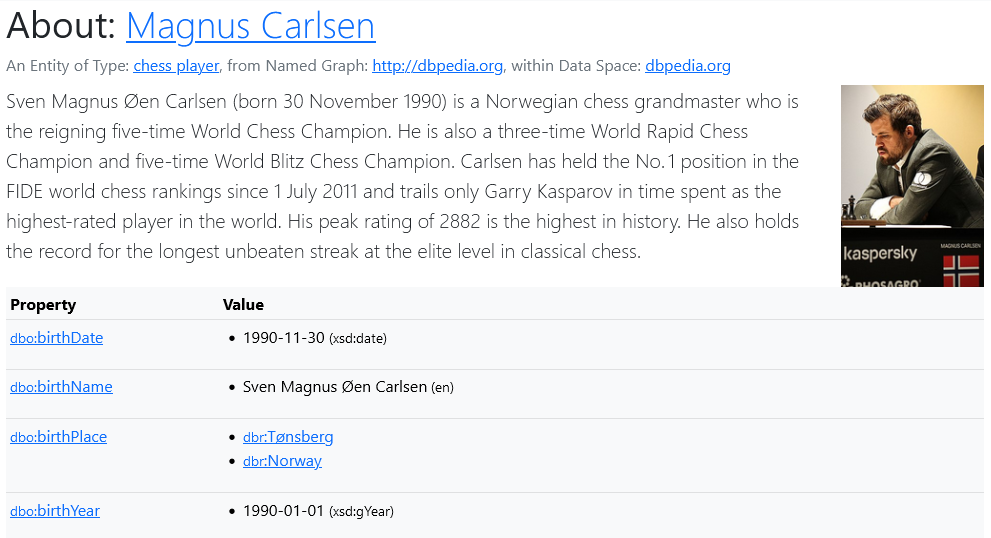
\includegraphics[width=\textwidth]{fig/kgs/dbpedia.png}
        \caption{The entity \textit{Magnus Carlsen} in DBpedia}
        \label{fig:kgs-dbpedia}
    \end{figure}

    \item \textbf{YAGO \cite{rebele2016}:} A Knowledge Graph that shares a number of similarities with DBpedia. Just like it, YAGO is also a KG that extracts semi-structured information from Wikipedia to create, as its authors put it, a \textit{``light-weight and extensible ontology with high quality and coverage''} \cite{suchanek2007}. A number of refinements are applied to the knowledge stored in YAGO, such as canonicalization, which removes possibly duplicate elements from the graph; or type checking, which prevents invalid combinations of entities from being formed.
    
    \item \textbf{FreeBase \cite{bollacker2008}:} A large-scale, multi-domain KG that aimed to collect human knowledge in order to facilitate its integration, usage and standardization. Unlike the previously discussed KGs, which use Wikipedia as their main sources of information, FreeBase was a collaborative project that relied on human editors and curators to add knowledge to it. It was also one of the first multimodal KGs, since it allowed users to include text, images and media files. FreeBase was acquired by Google in 2010 and, upon the release of the Google Knowledge Graph, it was discontinued and put in a read-only mode. However, it is still a popular Knowledge Graph in the academic domain, since many different research works use it to benchmark their proposals.
    
    \begin{figure}[!htp]
        \centering
        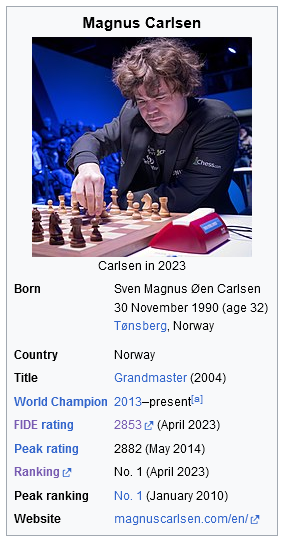
\includegraphics[width=.4\textwidth]{fig/kgs/infobox.png}
        \caption{A Wikipedia infobox}
        \label{fig:kgs-infobox}
    \end{figure}

    \item \textbf{WikiData \cite{vrandevcic2014}:} After KGs such as DBpedia and YAGO successfully leveraged the information in Wikipedia's infoboxes, the Wikimedia Foundation soon realized that the information contained in them could be very useful. However, the data in these boxes needed to be manually added, edited and updated by human editors, and constantly kept up-to-date in as many languages as the original articles were available in. To alleviate this issue, they introduced WikiData as a centralized and crowdsourced source of information, to supply Wikipedia articles and a number of other applications with data. Contrary to most other KGs, and following the philosophy of Wikipedia, all data entered into WikiData is not immediately considered a fact, but rather a claim that must be supported by references to outside sources. Both entities and relations in WikiData are denoted with codes, which makes it language-agnostic, but can reduce its human interpretability if they are not mapped to their human-readable names. Figure~\ref{fig:kgs-wikidata} shows a small excerpt of WikiData, centered around the entity \textit{Artist}.
    
    \begin{figure}[!htp]
        \centering
        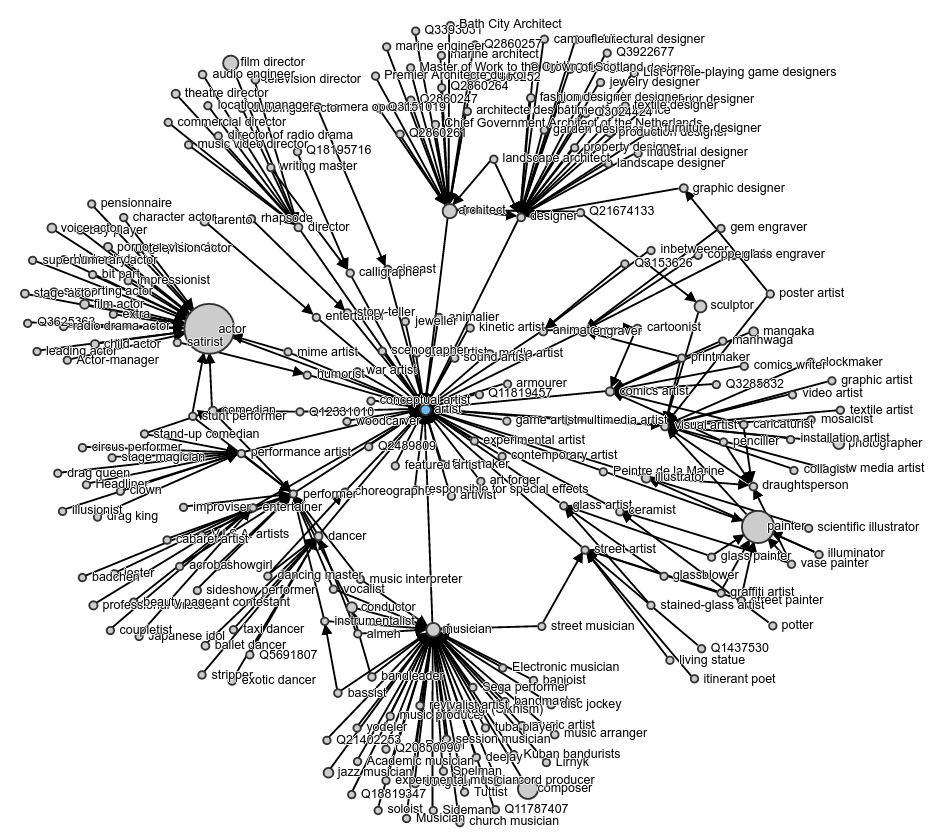
\includegraphics[width=\textwidth]{fig/kgs/wikidata.png}
        \caption{An excerpt of WikiData}
        \label{fig:kgs-wikidata}
    \end{figure}
    
    \item \textbf{NELL \cite{mitchell2018}:} The Never-Ending Language Learning project, or NELL for short, is a fully-automated system that scans the entire web, reads the contents of a webpage, and attempts to extract information from plain text written by humans. The information it extracts is then structured in the form of a triple and inserted in a KG. This Knowledge Graph is thus, by its very definition, under constant expansion. The NELL project allows users to rate an extracted fact positively or negatively, depending on whether or not the fact makes sense and is correct, and this allows the extractor to learn over time which facts are being successfully extracted, consistently improving its capabilities. NELL can also assign a confidence score to the facts it extracts, although only \textasciitilde6\% of its \textasciitilde50 million facts have a high confidence score.
    
    \item \textbf{MAKG \cite{sinha2015}:} A prime example of a domain-specific KG, the Microsoft Academic Knowledge Graph is a very large collection of over 8 billion triples with meta-information about research, such as academic publications, authors, institutions, and domains of study, among others. The information in it is obtained directly from two main sources: academic publishers, such as ACM and IEEE, and websites indexed by the Bing search engine, from which the information must be extracted from a plain-text format. In total, more than 83 million papers and 20 million authors are present in this academic Knowledge Graph.

\end{itemize}

\section{Applications}\label{sec:kgs-applications}
It has been established that Knowledge Graphs are a powerful tool to organize and connect information in a semantically meaningful way, making it easier for machines and services to understand and interpret complex data. The use of Knowledge Graphs has expanded rapidly across a wide range of fields, including healthcare, education, e-commerce, and many others \cite{peng2023}. By providing a structured representation of data, Knowledge Graphs enable more accurate and efficient decision-making processes, support natural language processing, and enhance the ability of machines to understand the context and relationships between different entities. 

In this way, Knowledge Graphs have proven to be an invaluable resource for a variety of practical applications that we take for granted nowadays, which require complex data management and analysis. Some of the most popular practical applications of Knowledge Graphs are as follows:

\begin{itemize}
    \item \textbf{Question answering:} Many search engines and personal assistants that are ubiquitous today, such as Siri, Alexa, Cortana, and Google Assistant, combine natural language processing (NLP) techniques, which helps them understand a query posed by a user, with Knowledge Graphs, which are used to navigate between entities and find the correct answer. Although most of the KGs that are used for this purpose are not made public for commercial reasons, they often contain a high amount of relations between both real-world and fictional entities and people. An example of this in practice is shown in Figure~\ref{fig:kgs-qa}.\\
    
    \begin{figure}[!htp]
        \centering
        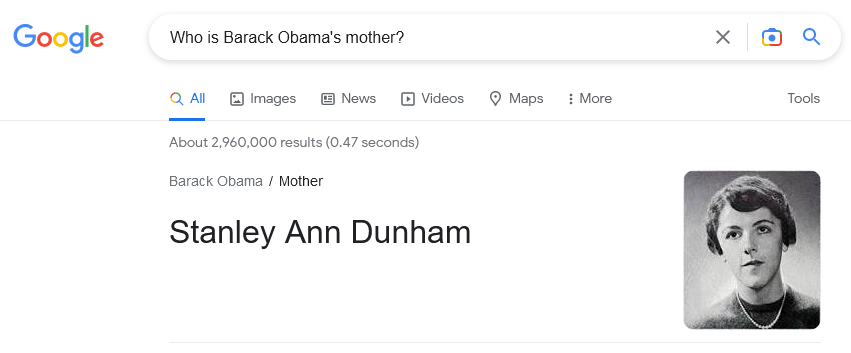
\includegraphics[width=\textwidth]{fig/kgs/qa.png}
        \caption{Question answering using the Google Knowledge Graph}
        \label{fig:kgs-qa}
    \end{figure}

    \item \textbf{Product recommendations:} Many authors \cite{zhang2021, palumbo2020, wang2019b, guo2022} have analyzed and proposed using Knowledge Graphs to issue product or media recommendations to users. By storing the relevant elements in a KG, such as the products that are on sale and the relations between them, and the users that bought or rated a product positively, one can apply a number of techniques to find a product that will be appealing to a new user in the system. The same concept can be applied for books or movies, a prime example of this is the movie information site IMDb, whose information has been used by Amazon to build a movie recommendation engine \cite{rele2022}.\newpage
    
    \item \textbf{Advanced information retrieval:} Traditionally, information retrieval systems work by building and maintaining an index of a collection of documents and, when a user submits a query to the system, returns the documents that match the query more closely. However, this purely text-based approach falls short when it comes to semantical problems, for example, disambiguating an entity in the query, or interpreting it correctly. For this reason, some authors have proposed using Knowledge Graphs to enhance this process: for example, during the recent COVID-19 outbreak, \citet{wise2020} introduced a COVID-19 KG that aggregated the most recently published scientific works regarding this disease. This KG could be queried to quickly retrieve relevant research efforts, facilitating a worldwide collaboration to quell the pandemic.\\
    
    \item \textbf{Education:} Multiple KG-centered proposals have been made in recent years to aid in several aspects of education. For example, \citet{chen2018} presented KnowEdu, a tool made for the purpose of building Knowledge Graphs out of educational materials. It is able to extract the main concepts of a subject or course, and then builds relations between them according to the activities and evaluation activities that the students will have to carry out in the future. \citet{aliyu2020} proposed building a KG containing the teachers, courses and scientific literature for a university, and using it to recommend relevant courses and books to students.\\
    
    \item \textbf{Research:} Besides the previously discussed MAKG, a number of other Knowledge Graphs of research and academic entities have been built to help researchers explore possible lines of investigation and find possible relevant related materials. AceKG, introduced by \citet{wang2018}, is a similar KG, containing more than 3 billion triples with information about authors, papers, venues, and so on. The Artificial Intelligence KG \cite{dessi2020aikg}, and its extension, the Computer Science KG \cite{dessi2022cskg}, also contain a large volume of information pertaining research concepts, materials, tasks, and other similar entities in these fields. Furthermore, \citet{angioni2021} introduced the Academia/Industry KG, to help researchers identify trends in the constant exchanges between these two realms.\\
    
    \item \textbf{Healthcare:} It is undoubtable that having an efficient and effective healthcare system is a cornerstone of a functional modern society. To help manage the ever-growing amount of medical data and records that healthcare professionals have to deal with, some proposals to integrate KGs in this field have been made. \citet{zhang2020b} presented HKGB, a KG builder aimed towards healthcare professionals that leverages their expertise to construct medical Knowledge Graphs. \citet{gong2021} proposed constructing KGs with information about medicines, diseases and patients, in order to use it to suggest medicines to patients with particular incompatibilities or intolerances. 
\end{itemize}

\section{Open challenges}\label{sec:kgs-challenges}
Despite the fact that Knowledge Graphs are already a well-established concept in research and industry, a number of challenges about their use and refinement still remain \cite{paulheim2017, hogan2020, peng2023}. In the following subsections, we delve into some of the most prominent ones in more detail. 

\subsection{Integration}
It is common that more than one Knowledge Graph contain information about the same real-world concept or entity. While each individual KG may include different additional information complementing it, it would be desirable that said information be integrated together, so as to have a single source of truth that contains a more comprehensive set of facts. The process of joining two or more Knowledge Graphs together is known as KG integration or fusion.

The most challenging step of this process is determining which entities in different KGs refer to the same one in the real world, a task known as entity alignment \cite{ren2022}. Although this has been a very active research topic, some future directions can still be further explored. For example, it is still not clear how this can be done reliably when the KGs to be integrated have different languages, which could be useful for multilingual recommendation systems or question answering \cite{javed2021}. An attempt in this regard has been made by \citet{xu2019} using neural networks, however, the alignment accuracy they obtain is still not high enough to perform this process reliably.

Moreover, most KG fusion approaches assume that the Knowledge Graphs to be fused together are of the same modality. This falls short in the presence of multi-modal KGs, for example, the previously discussed FreeBase. Joining together two or more KGs which entities can be represented in different formats is still an open challenge, although some authors have made recent proposals. \citet{guo2021} have presented HMEA, a multi-modal entity alignment technique by using hyperbolic spaces. \citet{cheng2022} proposed MultiJAF, a framework for multi-modal entity alignment. Despite this, the wide array of possible modalities that could be represented through a KG make multi-modal alignment a very challenging and still unsolved task.

Furthermore, a related problem is entity disambiguation. This problem presents itself during the process of building the KG, and consists in determining the specific meaning of an entity written in natural text in the presence of ambiguity. For example, contextual information is required to determine whether \textit{``Armstrong''} refers to the astronaut, the jazz musician, or the cyclist. If this is not solved correctly, even a successful entity alignment can be poisoned by the fact that the entities that were aligned were not disambiguated properly upon their creation, and thus do not actually refer to the same concepts.

\subsection{Correction}
The previous analysis of the most popular Knowledge Graphs shows that automatic construction is the most common way to build a KG, due to the sheer amount of facts that they are intended to contain. It is therefore inevitable that these automated methods introduce a certain degree of incorrect information in the KG, either because it was not correctly interpreted, or because the original source of information was wrong.

Refining a KG after its creation by detecting wrong facts is known as Knowledge Graph correction. The most common way to perform this task is to do fact validation \cite{paulheim2017}, which assigns a confidence score in the interval $[0, 1]$ to every triple in the KG. Then, the triples that do not meet a minimum confidence threshold are purged from the graph.

There exist a number of research works in the literature that propose different ways to do fact validation. \citet{pasternack2010} propose converting the facts in a KG into natural language sentences, and then using more general methods for fact checking. The same authors \cite{pasternack2011} also propose an alternative method, which groups up similar facts in a KG that provide support for each other, and then joins these groups to create more general justifications for the possible correctness of a fact. \citet{gerber2015} have proposed using classifiers, which can learn which facts are wrong by using a number of features. Of course, this requires that a manually-annotated set of correct and wrong triples is provided, which can be an arduous task. Another classification-based approach is proposed by \citet{syed2018}, in this case, based on textual evidence.

A more refined ---and challenging--- approach to KG correction is to not only detect which facts are wrong, but to amend them if possible so that they represent correct knowledge. This is known as fact repairing. Due to the increased difficulty of the task, a smaller body of work can be found in the literature. \citet{topper2012} proposed leveraging the ontology of a Knowledge Graph to detect and fix inconsistencies in triples where the domain or range restrictions of the relation are violated, however, their proposal requires a human to step in and select the correct version of it out of the suggestions provided by the system. \citet{bonatti2011} proposed a fully-automated method for fixing triples, but it requires provenance and trust annotations to be present in the KG, which are relatively rare.

\subsection{Completion}
As previously discussed, most KGs are commonly built by extracting non-structured or semi-structured information from web sources, though some KGs can be manually curated by domain experts. When information extraction systems are applied to extract knowledge from online sources, that information is then semantized~\cite{ayala2018, neumaier2016} and stored in a KG as triples in the KG. Regardless of the specific process by which a KG is constructed, the resulting graph usually lacks a certain amount of information, either because said information was not originally present in the information source, or because it was unsuccessfully extracted or semantized~\cite{bordes2014b}. 

Because of this inherent incompleteness, KGs operate under the Open World Assumption, i.e., a piece of information that is not present in a KG is not considered to be incorrect, but rather just unknown~\cite{galarraga2015}. Therefore, it is mandatory to refine KGs after their creation in order to expand the knowledge they contain~\cite{paulheim2017}.

Deriving additional knowledge from an existing KG with the goal to augment it is a task known as Knowledge Graph completion~\cite{paulheim2017, shen2022overview}. In KG completion, the goal is to identify triples that are missing from the KG and have a chance of being correct that is as high as possible. To achieve this goal, a series of steps are usually carried out, which are visually depicted in Figure~\ref{fig:kgc-workflow}.

\begin{figure}[!htp]
    \centering
    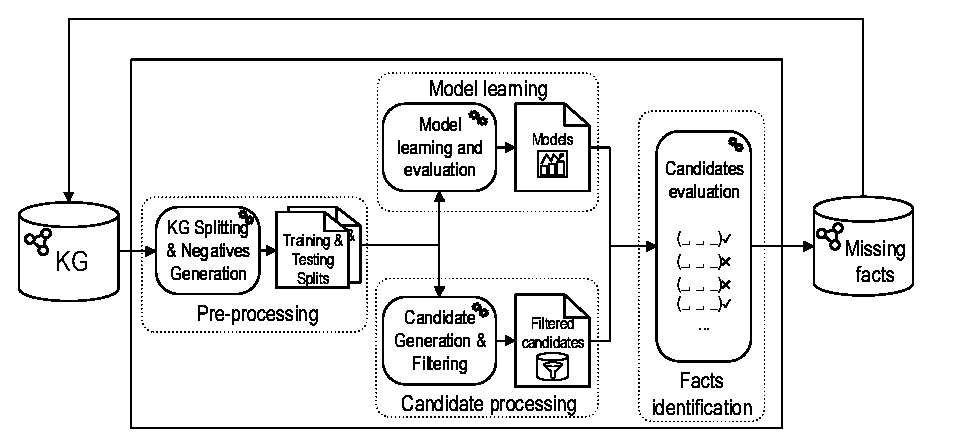
\includegraphics[width=\textwidth]{fig/kgs/kgc_workflow}
    \caption{Knowledge Graph completion workflow}
    \label{fig:kgc-workflow}
\end{figure}

First, the Knowledge Graph must be pre-processed in order to add negative triples, in the case they are not present, and split them between a training and a testing set \cite{ayala2019}. Then, a KG completion model is trained and evaluated using the sets of triples generated in the previous step. In parallel, a set of plausible candidate triples is materialized. If the KG completion model yields a satisfactory efficacy after its evaluation, it is applied on the candidate triples, to identify which ones are correct and which ones should be discarded \cite{borrego2021, borrego2019,shen2022overview}. Finally, the triples considered correct are added back to the Knowledge Graph, enriching it.

In opposition to the previous two challenges, which focus on information that is already present in the graph, KG completion, by definition, focuses on finding knowledge that is not yet present. For this reason, it is particularly hard, and a number of authors have made different proposals to tackle it. Since the focus of this dissertation is on Knowledge Graph completion, the following chapters provide a more in-depth analysis of the existing proposals in the scientific literature to complete Knowledge Graphs.

\section{Summary}\label{sec:kgs-summary}
This chapter has introduced the reader to Knowledge Graphs. It has provided a brief summary of their history and main characteristics, as well as a summary of the most prominent KGs that can be found today. Furthermore, it has presented the reader with an ample repertoire of practical applications of Knowledge Graphs, many of which we use in our daily lives. Finally, it has introduced some of the challenges regarding KGs that still remain open to this day, namely: Knowledge Graph integration, correction, and completion.

    \chapter{Latent triple representations}\label{chap:embeddings}

\chapterQuote{\textit{``All problems in computer science can be solved by another level of indirection, except for the problem of too many layers of indirection.''}}{--- David Wheeler}

I dont like the name of this chapter, but I assume it was changed from Embeddings as to make it easier to non expert readers?

\chapterAbstract{E}{sta seccion habla de embeddings y como funcionan.
La que acabe estando en la version final de la tesis debe de ser bastante similar a la presentada x agu ya que el mundo de los embeddings no se ha movido mucho y se usan para practicamente lo mismo en ambas propuestas.}

Quizas moveria las prpuestas a una misma categoria mas general y pondria una tabla explicando los progesos de cada una de las ramas y luego entraria en detalles sobre las mas novedosas que hay ( y sobretodo en las que se han usado en el trabajo...)
% latent representation of a triple is one that exposes previously hidden knowledge, such as semantic similarity to some other triple. Obtaining such a representation is a popular way to perform Knowledge Graph completion, and it can be achieved in a number of ways. In this chapter we introduce the most prominent KG completion methods in the scientific literature that rely on latent representations. This chapter is structured in the following manner: Section~\ref{sec:emb-intro} provides an introduction to the matter, Section~\ref{sec:emb-tensors} presents the methods that perform  tensor factorization, Section~\ref{sec:emb-translations} introduces the models that are centered around embedded translations, Section~\ref{sec:emb-nn} discusses the number of ways in which neural networks can be used in this regard; finally, Section~\ref{sec:emb-summary} provides a summary of the contents of the chapter.

\section{Introduction}\label{sec:emb-intro}
que son y porque se usan en los grafos de conocimiento.

% A popular approach to Knowledge Graph completion consists on changing the representation medium of entities and relations entirely: instead of elements with a semantic meaning in a graph structure, they are represented in a numerical way. This then allows for the application of numerical methods to find missing entities, or missing connection between the existing entities. This is known as a latent representation.

% One such way is by using tensors, a mathematical structure that can hold data in any number of dimensions. Consequently, through a series of transformations, the original tensor representing the Knowledge Graph is turned into another that materializes some knowledge that was not previously readily available.

% Another popular latent representation is by creating an N-dimensional space and determining a position in it for every entity in a KG. An entity can then be referred to as the N-dimensional vector that represents its position. Such a space is known as an embedded space, and the position vectors are known as entity embeddings. In the embedded space, the plausibility of any given relation can be checked by performing a series of translations in it and evaluating the result, or by finding more complex relations between the entity embeddings thanks to the use of neural networks.

\section{Tensor factorization models}\label{sec:emb-tensors}
Rescal, SimplE, ComplEx etc etc...

% Tensors are a generalization of scalar numbers, vectors, matrices, and so on. Broadly, a tensor of order $N$ represents an $N$-dimensional collection of elements, where $N$ indices are necessary to address the position of an element. Any given Knowledge Graph can be represented using a third-order tensor of size $|E| \times |E| \times |R|$, namely $X = \{0, 1\}^{|E| \times |E| \times |R|}$, where $E$ is the set of entities in the KG, and $R$ is the set of possible relations in it. Using this representation, every element of the tensor is a binary number $\{0, 1\}$ denoting whether or not a given relation exists between a pair of entities. This concept is visually represented in Figure~\ref{fig:emb-kg2tensor}.

% \begin{figure}[!htp]
%     \centering
%     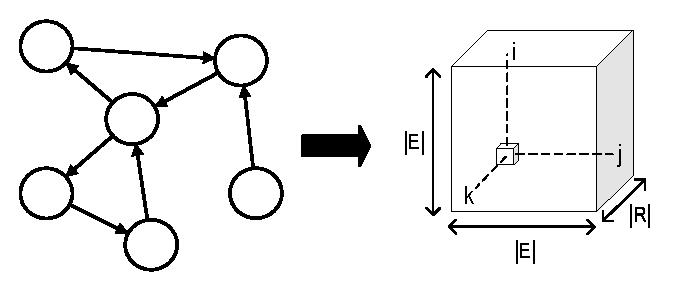
\includegraphics[width=.9\textwidth]{fig/embedding/kg2tensor}
%     \caption{Representing a KG as a third order tensor}
%     \label{fig:emb-kg2tensor}
% \end{figure}

% Once this representation is achieved, the goal of tensor factorization models is to compute a complementary tensor $Y = [0, 1]^{|E| \times |E| \times |R|}$ representing the correctness confidence of all possible combinations of entities and relations. Note that the elements in $X$ are binary, while those in $Y$ can take any real values between 0 and 1. Finally, to complete the KG, the facts with the highest confidences in $Y$ that are not still present in the Knowledge Graph are added into it.

% One of the first models in this line of work is RESCAL, which was proposed by \citet{nickel2011}. RESCAL represents the data in a Knowledge Graph using a tensor with the same structure as that shown in Figure~\ref{fig:emb-kg2tensor}. Then, it creates 2-dimensional slices of this tensor, one per each relation, which are illustrated in Figure~\ref{fig:emb-rescal}. Each slice, $X_r$, is factorized as $X_r = AB_{r}A^{T}$, where $A$ is a matrix that contains the latent representations of the entities, and $B$ is another matrix that represents the interactions of said entities for the relation $r$. Then, to predict the existence of a relation in them, the confidence scores are looked up in the computed latent representations.

% \begin{figure}[!htp]
%     \centering
%     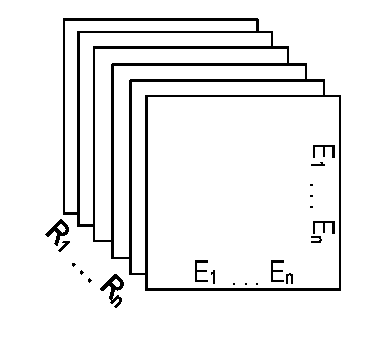
\includegraphics[width=.4\textwidth]{fig/embedding/sliced}
%     \caption{A third order tensor, sliced up in the RESCAL model}
%     \label{fig:emb-rescal}
% \end{figure}


% \citet{jenatton2012} proposed the LFM model, an extension of RESCAL that scales better to Knowledge Graphs with a higher number of relations. Similarly to the model it builds upon, LFM represents the tensor as a series of $X_r$ slices, but introduces a more complex factorization based on a bilinear structure that is able to capture one-, two-, and three-way interactions between the components of a triple. Additionally, the matrix that represents the interactions between the latent representations of the entities is further decomposed into smaller elements, which reduces the number of parameters required for its computation and thus increases the efficiency of the model.

% A combination of the previously discussed two approaches is proposed by \citet{garcia-duran2015}, who introduced the Tatec model. Tatec has features of both RESCAL and LFM, learning two different embedded representations of the same Knowledge Graph and combining their confidences together as $score(s, r ,t) = s_1(s, r, t) + s_2(s, r, t)$, where $(s, r ,t)$ can be any triple, and $s_1, s_2$ are the score functions of a bilinear and trilinear tensor factorization model, respectively. Naturally, the scores emitted by both models must be normalized before they can be combined. The authors also suggest and benchmark a series of possible alternative ways to combine the scores of the two constituent models within Tatec.

% \citet{liu2017} proposed the ANALOGY model, which is also an extension of RESCAL. ANALOGY derives its name from its focus on modelling and analyzing the analogical properties that are captured in the embedded representations of the entities. ANALOGY imposes further restrictions upon the relationship matrices of RESCAL, $B_r$, by demanding that they be normal ($B_rB_r^T = B_r^TB_r$) and commutative ($B_rB_{r'} = B_{r'}B_r$). This enables them to efficiently be block-diagonalized into a set of smaller matrices, which the authors show that enables them to be used in mathematical formulations of a lower complexity. Additionally, the factorization process of ANALOGY is guided by a fully-differentiable goal, which increases its computational scalability. 

% A similar effort was carried out by \citet{yang2014}, who introduced the DistMult model. The authors of DistMult propose replacing the dense $B_r$ matrix of the RESCAL model with a diagonal matrix, which greatly reduces its number of parameters and allows for a much speedier execution.

% \citet{tay2017} introduced the REST factorization model, which is especially tailored for large Knowledge Graphs. REST relies upon random walks to sample small subgraphs within the KG, and represents these subgraphs using tensors. The subgraphs are further split up using a relation sparsification technique, yielding even smaller tensors. The tensors representing different parts of the KG are combined together to produce an ensemble model that can be representative of the entire Knowledge Graph. This ensemble architecture is visually depicted in Figure~\ref{fig:emb-ensemble}. REST has provided satisfactory results in practice, and its ability to work on-demand make it a convenient choice for Knowledge Graphs that are in continuous expansion.

% \begin{figure}[!htp]
%     \centering
%     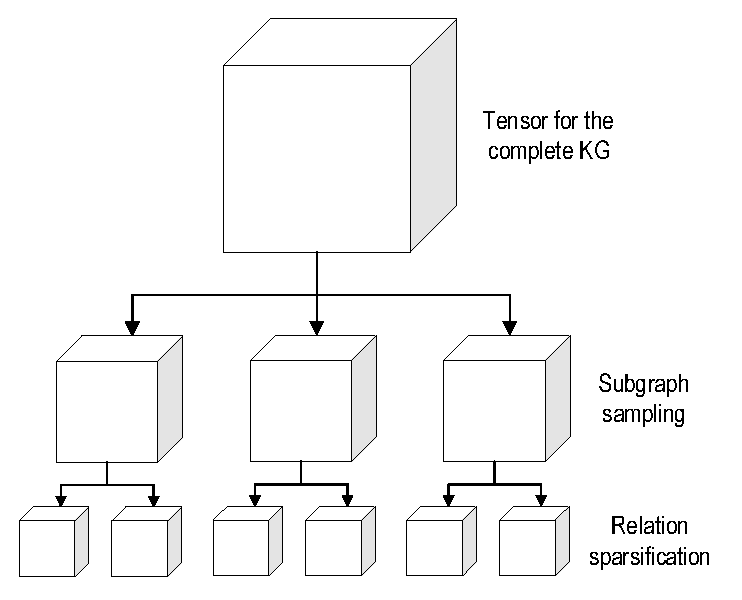
\includegraphics[width=.7\textwidth]{fig/embedding/ensemble}
%     \caption{An ensemble of tensors, as proposed by the REST model}
%     \label{fig:emb-ensemble}
% \end{figure}


% \citet{trouillon2016} proposed the ComplEx model, which is the first one to use complex instead of real values in the tensors. This can also be seen as splitting an embedded representation of the entities into two: one which contains the real values of the numbers, and one that contains the imaginary parts. This increases the expressiveness of the model, and makes it better suited to handle symmetric and antisymmetric relations, which are traditionally more challenging for the previously discussed models, due to the fact that they greatly increase the number of parameters they must deal with \cite{nickel2011, socher2013}. Perhaps counterintuitively, the use of complex numbers simplifies its score function, since it only uses the Hermitian dot product, which is the equivalent in $\mathbb{C}$ of the standard dot product in $\mathbb{R}$.\newpage

% Perhaps inspired by the naming of the previous model, \citet{kazemi2018} introduced the SimplE model, which aims to be more performant than other approaches in this category. For each relation $r$ present in a KG, SimplE considers an additional inverse relation $r^{-1}$ to it. Both are then represented using the vectors $v_r$ and $v_r^{-1}$, respectively. Thus, the confidence score for a triple $(s, r, t)$ is computed as the average of the confidence of $(s, r, t)$ and $(s, r^{-1}, t)$. This configuration allows the embedded representation of a relation and its inverse to be obtained independently, resulting in a higher expressivity and a good performance in practice.


\section{Translational models}\label{sec:emb-translations}

TransE, TransR y un muy larguisimo etc...

% A separate group of models represent entities as vectors in an N-dimensional space, called embeddings, and relations as translations in that space. From this starting point, their main goal is to define the transformations from entities to vectors and the translations in such a way that, for every triple $(s, r, t)$ in the KG, applying the translation defined by $r$ to the entity $s$ should result in a vector as close as possible to that of $t$. These models can then be used to provide a confidence value for the correctness of any triple, by evaluating to what extent this concept holds true.

% \citet{bordes2013} started this line of work with the TransE model. TransE defines a single N-dimensional space to which all entities in a KG are mapped, and in which every relation turns into a translation vector. Thus, it aims to generate this space in such a way that, for any given triple $(s, r, t)$, $v_s + v_r \approx v_t$, where $v_s, v_t$ are the vectors representing the $s$ and $t$ entities respectively, and $v_r$ represents the translation carried out by the relation $r$. The main intuition behind TransE is visually depicted in Figure~\ref{fig:emb-transE} for a simple 2D space.

% \begin{figure}[!htp]
%     \centering
%     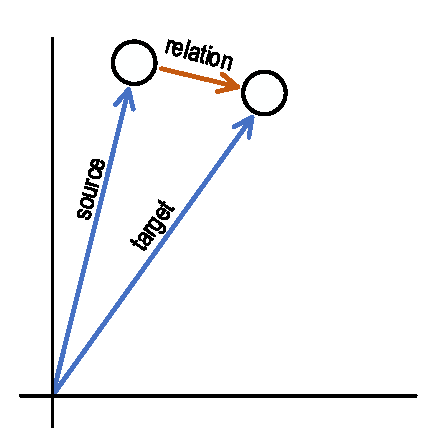
\includegraphics[width=.4\textwidth]{fig/embedding/transe}
%     \caption{Visual representation of the TransE model in a 2D space}
%     \label{fig:emb-transE}
% \end{figure}

% \citet{wang2014} proposed the TransH model, which improves TransE by considering that it may desirable for an entity to have a different embedded representation depending on the particular relation that is being considered. TransH achieves this by defining a particular hyperplane $w_r$ for every relation $r$, and then projecting the entities onto these planes as $e_\bot = v_e - w_r^{T}v_{e}w_r$, where $e$ can be any entity in the KG. Then, similarly to TransE, it optimizes the embedded space to ensure that $s_\bot + v_r \approx t_\bot$ for any triple $(s, r, t)$. A similar visual representation is provided in Figure~\ref{fig:emb-transH}.

% \begin{figure}[!htp]
%     \centering
%     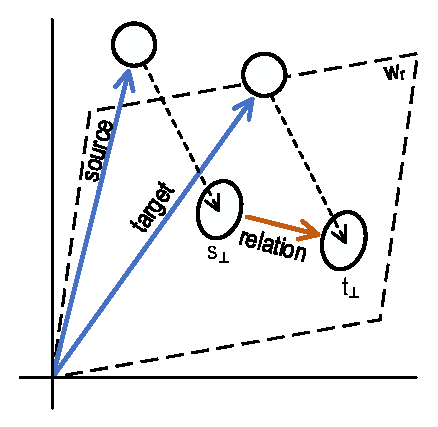
\includegraphics[width=.4\textwidth]{fig/embedding/transh}
%     \caption{Visual representation of the TransH model in a 2D space}
%     \label{fig:emb-transH}
% \end{figure}

% Following up with the previous idea, \citet{lin2015} proposed the TransR model. It acknowledges that an entity and a relation have a very different semantic meaning and, for this reason, TransR makes a twofold contribution. On the one hand, it defines two separate embedded spaces, one for entities and one for relations. On the other hand, it creates a different entity embedded space for each relation. The transition from the entity space to the relation space is performed through a relational projection matrix $M_r$. The translation goal thus becomes $v_sM_r + v_r \approx v_tM_r$. A graphical example of this is provided in Figure~\ref{fig:emb-transR}.

% \begin{figure}[!htp]
%     \centering
%     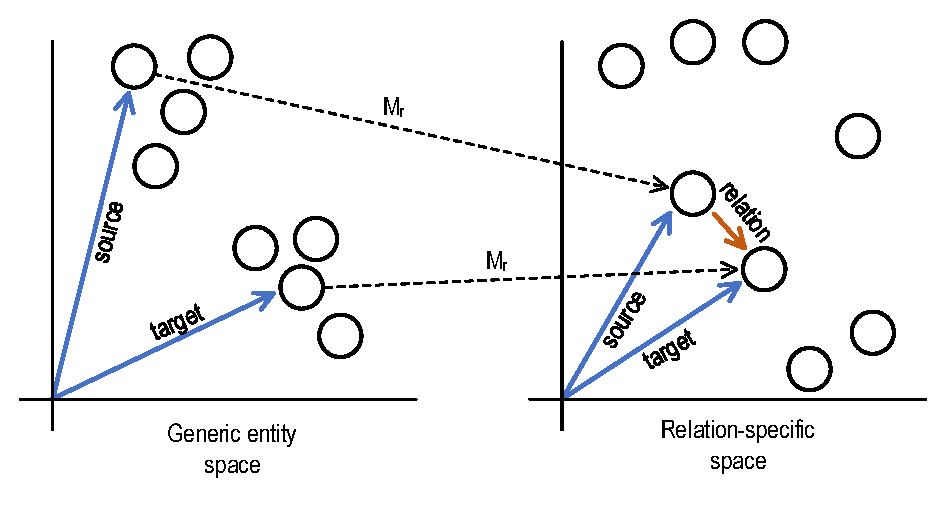
\includegraphics[width=.85\textwidth]{fig/embedding/transr}
%     \caption{Visual representation of the TransR model in a 2D space}
%     \label{fig:emb-transR}
% \end{figure}

% \citet{ji2015} introduced the TransD model, building upon TransH and improving it by constructing mapping matrices dynamically for every entity. Furthermore, it replaces the matrix multiplication operations used in the previous models with vector multiplications, which increases its operational speed. A similar approach is proposed by \citet{do2018} with TransF, which uses more lightweight matrices to perform the translation.

% \citet{fan2014} devised TransM, addressing the fact that the original TransE proposal considers all triples to be equally important, and thus they all contribute equally towards generating the embedded space in such a way that it optimizes the transformation goal. TransM adds a weight parameter that can be assigned to every individual triple, which affects its ability to influence the embedded space as a whole and acts as an attention mechanism.

% \citet{xiao2015} presented the TransA model, which uses an adaptive goal metric during the embedding generation process, overcoming the simple metrics used by other similar methods, making it more flexible when facing challenging relations.

% Perhaps facing the prospect of running out of letters in the English alphabet to continue with the previous naming scheme, \citet{sun2019} proposed the RotatE model, which defines an embedded space that uses complex numbers. Contrary to the previous models, where a translation is defined as a straight movement through the space, RotatE defines each relation as a rotation on the whole embedded space.

\section{Neural network-based models}\label{sec:emb-nn}
Como se aplican los embeddings a KG reasoning/completion. 

% In parallel to the development of research centered around Knowledge Graphs, the fields of neural networks (NNs) and deep neural networks (DNNs) have also seen significant improvements in the last decade \cite{vaswani2017, brown2020, rombach2022}.

% Consequently, a number of NN and DNN architectures have been applied to the problem of completing a Knowledge Graph, by virtue of transforming a triple into a representation that can be consumed by these models, and training them so that they can learn what constitutes correct knowledge. Contrary to the previously discussed translation-based models, NN models apply non-linear transformations to the data they are provided. This can result in an increased ability to deal with more complex data, however, it also makes their reasoning harder to understand.

% One of the first models that were proposed in this regard was NTN, by \citet{socher2013}. This model relies on a pre-computed set of word embeddings, in which semantically similar words are expected to be close to each other in the embedded space. NTN takes all the meaningful words in the name of an entity and averages the respective word embeddings together, resulting in a single embedding for every entity. In this manner, the embeddings of the two entities of a triple are provided as input to a bilinear neural network, which then outputs a confidence score for the entity pair. However, NTN is dependent on the availability and quality of the aforementioned word embeddings. Furthermore, these embeddings must be computed again if an entity with a novel word in its name is introduced in the Knowledge Graph. 

% A simplified version of NTN is used by \citet{dong2014} in their Multilayer Perceptron (MLP) proposal. MLP is used in the Google Knowledge Vault, a KG created by the same authors, to filter out possibly incorrect facts that are automatically extracted from plain text around the Web. To make it more lightweight in order to be applied to such a large KG, MLP changes the interaction function used by NTN to a multi-layer perceptron, which is much faster to train.

% A further refinement is proposed by \citet{liu2016}, who introduced the Neural Association Model (NAM). It uses deep neural networks to learn and infer the joint conditional probabilities between two facts. One of the main strengths of NAM is its increased explainability, since using conditional probabilities makes it easier to justify the correctness of a triple using other triples known to be correct as supporting evidence.

% \citet{guan2018} proposed a Shared Embedding-based neural network (SENN) for the task of KG completion. SENN aims to achieve a higher level of specialization by using three separate neural sub-structures to predict a missing source entity, relation, or target entity in a triple. The results of these structures are combined together to assess the correctness of a whole triple. By virtue of being an ensemble of smaller structures, SENN is also more efficient than some of the other pre-dating models.

% The interconnected nature of Knowledge Graphs also calls for the application of convolutional neural networks (CNNs). These networks do not focus on only one entity at a time; they are also able to derive information from other entities close to it, having a larger picture of the KG as a whole. In this line, \citet{dettmers2018} introduced ConvE, a two-dimensional CNN that operates on the entire matrix that represents entity embeddings. ConvE uses a traditional 2D convolution to augment its predictive capabilities with respect to more classical NN architectures. It also has a more reduced number of parameters that must be trained, increasing its efficiency.

% An evolution of ConvE is the InteractE model, proposed by \citet{vashishth2020}. InteractE uses a novel circular convolutional structure, which enables it to capture more meaningful interactions. \citet{nguyen2019} also build upon the main idea of ConvE to introduce CapsE, a method that works by using a capsule network \cite{sabour2017} that converts the entities of a Knowledge Graph into images, and then performing more traditional 2D convolutions on said images.

% In more recent years, graph convolutional networks, also called simply graph neural networks (GNNs) have emerged as a way to apply NNs to graph-like structures \cite{bruna2014, wu2021, zhou2020, kipf2017}. It seems thus reasonable that Knowledge Graph completion could benefit from the application of GNNs \cite{ye2022}. %Recently, \citet{TODO fernando} have studied the application of GNNs to KG completion and other related tasks, reaching the conclusion that they can generally outperform traditional neural networks, although more work and fine-tuning is needed to achieve consistent results.

% In this regard, \citet{schlichtkrull2018} proposed R-GCN, a type of GNN that leverages graph neighborhoods in order to complete them. \citet{shang2019} have proposed SACN, an encoder-decoder method based on this type of NN. For encoding, SACN uses a composition of multiple weighted GNNs that is able to leverage information from the structure of a Knowledge Graph and the attributes contained in its entities. The decoder uses a modified version of the previously mentioned ConvE model. The addition of GNNs allows it to outperform the original ConvE method.

\section{Summary}\label{sec:emb-summary}
% In this chapter, we have presented an overview of the existing methods for Knowledge Graph completion in the literature that rely on latent triple representations. We have introduced and described the models that use tensors to model a KG, and then factorize those tensors to obtain a predictive model. We have also presented the models that embed entities in a higher-order space and perform translations on them to find missing knowledge. Finally, we have enumerated the methods that use neural networks to perform Knowledge Graph completion, and we have presented the neural network architectures that are commonly used for this task.

brief summary of all the facts presented.
    \chapter{Path-based approaches}\label{chap:paths}

\chapterQuote{
    \textit{``Caminante, no hay camino, se hace camino al andar.''}\\
    \textit{(``Traveler, there is no path, you make your path as you walk.'')}
    }{--- Antonio Machado}

\chapterAbstract{P}{aths between entities are ubiquitous in any Knowledge Graph. For every entity pair, there are most likely a considerable number of distinct paths that connect them together. By analyzing these paths, many existing proposals are able to learn which pairs of entities should be linked together, and which ones have no direct connection whatsoever. Furthermore, paths can be used to navigate the neighborhood of an entity and extract information from it. In this chapter, we summarize the existing proposals for Knowledge Graph completion that leverage path information. It follows this structure: Section~\ref{sec:path-intro} introduces the reader to the basic concepts, Section~\ref{sec:path-relational} presents the proposals that are centered around using only information derived from paths, Section~\ref{sec:path-neighborhood} introduces the methods that analyze entity neighborhoods, Section~\ref{sec:path-hybrid} provides an overview on the proposals that combine latent representations with path-based information and, finally, Section~\ref{sec:path-summary} concludes this chapter.}

\section{Introduction}\label{sec:path-intro}
% A relational path is a sequence of relations that connect two entities together in a Knowledge Graph. There can be many such paths between any two entities, and they can vary in length and complexity. Given that these paths can provide an interesting insight on how related two entities are, many researchers have developed methods to analyze them to learn what constitutes correct knowledge. 

% Generally, these methods generate features that characterize the information contained in each path, and then train classifiers to predict the existence of missing relations based on these features. Due to the high number of possible paths that can exist between two entities, such methods usually use techniques like random walks to restrict the amount of paths that are analyzed, possibly constraining their effectiveness.

% To solve this issue, other methods analyze graph neighborhoods, which refer to the entities and relationships that are directly connected to a given entity in a Knowledge Graph. This allows KG completion method to focus on a much more reduced amount of information that is more likely to accurately characterize an entity.

% In this chapter, we present an overview on the methods that rely on these techniques to complete a Knowledge Graph. We first introduce the methods that rely purely on relational paths and their characterization. Next, we present the methods that analyze entity neighborhoods. Finally, we discuss more advanced methods that combine these approaches with techniques from the previous chapter.

\section{Using relational paths}\label{sec:path-relational}
% A relational path is simply a concatenation of triples that connect an entity to some other entity through a number of relations. Naturally, any Knowledge Graph has an abundance of possible paths to, from, or between entities. The idea of analyzing such paths to learn what constitutes valid knowledge has led to many research works.

% One of the first approaches that exploited relational paths in a Knowledge Graph was the Path Ranking Algorithm (PRA), proposed by \citet{lao2011}. PRA uses random walks to generate a set of paths between a given pair of entities in a depth-first manner. The generated paths are then transformed into a series of features that aim to characterize the information contained in it. These features are ultimately used to train a binary log-linear classifier, which learns whether a direct relationship should exist between two entities according to the paths that are already present between them. However, PRA is not without limitations. The number of possible paths between a pair of entity can be very high, limiting its scalability. Additionally, the randomly guided paths that it uses may miss information just by mere chance.

% Aiming to improve PRA, \citet{gardner2015} introduced the Subgraph Feature Extraction (SFE) method. In opposition to PRA, SFE uses a breadth-first search that is not randomly guided, in order to better characterize the portion of the KG between two entities. SFE also requires the creation of a handmade ``Alias'' relation, which relates entities in the same KG that refer to the same element in the real world. It is able to achieve more expressive results than PRA, making it easier for the human user to understand what constitutes a good path that may be indicative of the existence of a direct relation between two entities.

% \citet{gardner2013} also proposed an extension of PRA that addresses the issue of potentially having to consider a very high number of paths. It considers the semantic similarities between the relations of a Knowledge Graph, and uses them to merge very similar paths together, greatly reducing the number of paths that need to be analyzed afterwards. This addition increases the effectivity of PRA in the NELL Knowledge Graph, although the authors do not provide data for any other KGs.

% \citet{nastase2019} proposed the Abstract Path Model (APM), which produces an abstract graph from a KG, and then focuses on extracting relevant abstract paths from it. These abstract graphs provide a more general representation of the high-level relations between entities, and thus the paths that can be traced in it represent more high-level knowledge. Additionally, this abstract representation is, as a general rule, considerably smaller than the KG it is derived from and not very computationally taxing to obtain, which aids in its application to larger graphs.

% \citet{gu2015} introduced the Trans-COMP method, which proposes a different strategy. Rather than analyzing a large number of paths between two entities to try to characterize the pair, it only uses a single path. Precisely, it aims to select the path that provides the highest predictive capabilities of the existence of a given relation. \citet{toutanova2016} further refine this idea with their All-Paths method by providing an explicit way to represent the intermediate entities that can be found in such a path and, additionally, enabling the method to consider more paths.

% A number of other authors have also researched alternative ways to select and learn from the best paths in a Knowledge Graph. \citet{jiang2017} proposed the APCM model, which assigns different weights to the found paths and combines them based on these weights. Furthermore, the PRCTA model introduced by \citet{lei2019} employs an attention mechanism \cite{vaswani2017} to construct and select the paths, which allows it to work satisfactorily in more sparse KGs.

% \section{Using entity neighborhoods}\label{sec:path-neighborhood}
% Considering the possible paths between two entities is undoubtedly helpful, but this concept can be expanded further. Rather than a single path, we can consider the entirety of the region of a Knowledge Graph around a certain entity, in other words, its neighborhood. The concept of entity neighborhood is visually shown in Figure~\ref{fig:path-neighborhood}, which depicts the closest and more extended neighborhoods of an entity shown in the center.

% \begin{figure}[!htp]
%     \centering
%     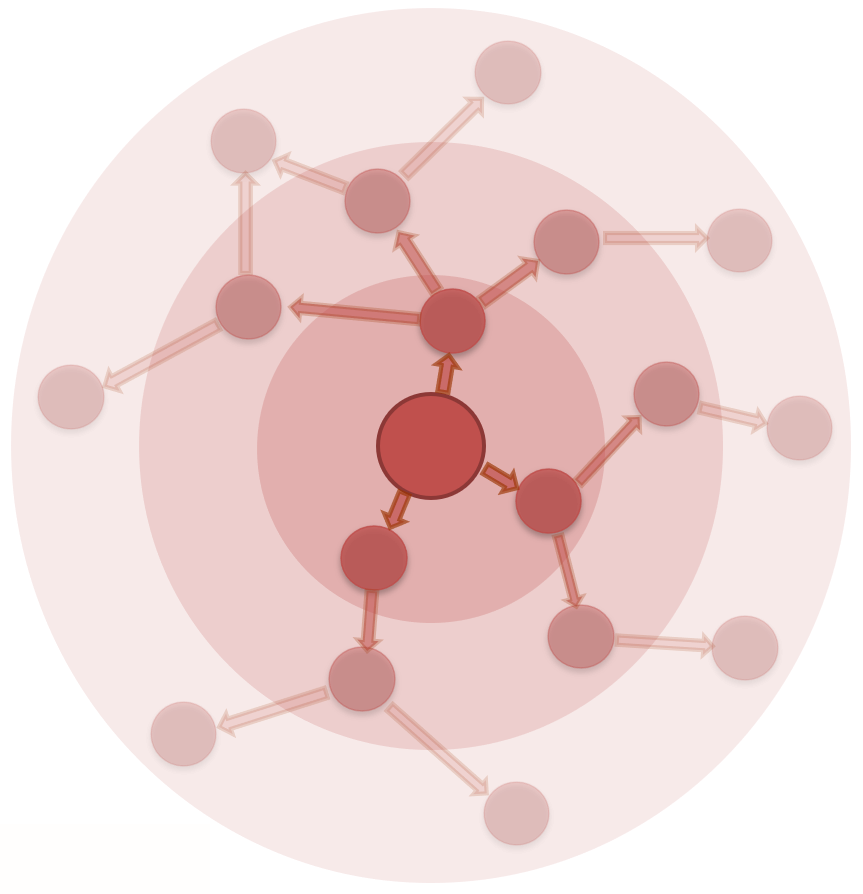
\includegraphics[width=.7\textwidth]{fig/paths/neighborhoods-b.png}
%     \caption{A visual representation of entity neighborhoods}
%     \label{fig:path-neighborhood}
% \end{figure}


% Given a pair of entities, their neighborhoods can be analyzed to determine if a relation should be present between them. This idea has been put to practice by a number of authors.

% \citet{bansal2019a2n} proposed the A2N method, which aggregates the entities in a neighborhood together to obtain a more compact representation of said neighborhood. It uses an attention-based mechanism to focus on the most prominent entities, giving a trustworthy representation of the entities surrounding another one. Additionally, it is designed such that the computational cost of the method does not increase greatly with the size of the neighborhoods.

% The use of attention-based mechanisms in this regard has not gone unnoticed by other authors. \citet{wang2019} have proposed LAN, another approach that aggregates the contents of an entity neighborhood together, however, the attention-based technique that they propose uses weights to give more importance to more relevant entities. \citet{kong2019} also proposes using attention to filter out possibly irrelevant relations in the graph, allowing the models to focus only on more meaningful information, which is especially relevant in the case of heterogeneous Knowledge Graphs. Similarly, \citet{nathani2019} introduced the KBAT method, which is able to capture information from both the entities and the relations in a KG neighborhood. 

% \citet{zhang2020} further the previous idea by adding a weighted attention system to both entities and relations, acknowledging that not all knowledge in the KG is equally useful. Two different attention-based mechanisms are used in their proposal. First, the relation-level attention provides an intuition for which connections from an entity may provide more useful information. Then, the reached entities are considered according to their entity-level attention. This composite, hierarchical attention mechanism allows it to outperform other attention-based proposals.

% \citet{ferre2019} proposes finding missing information by finding similar entities in commonly occurring graph patterns, through the application of concepts of nearest neighbors \cite{denoeux1995}. It does not require any sort of pre-processing of the Knowledge Graph, making it very efficient. Furthermore, its reliance on graph patterns makes it a more interpretable method than other similar proposals.

\section{Hybrid approaches}\label{sec:path-hybrid}
% The previous chapter introduced the main ideas behind how embeddings and neural networks can be applied to Knowledge Graph completion. Some authors have proposed a series of approaches that combine path-based information with these techniques, in order to guide the path finding process towards the most significant path, avoiding having to explore a very large number of them.

% An example of this is the PATH-RNN technique, which was proposed by \citet{neelakantan2015}. In addition to using path-based information, PATH-RNN uses the embedded representations of the relations in a path to further characterize it. It uses a recursive neural network (RNN) to combine these embeddings together, resulting in a single embedding that contains information about the entire path. For this reason, it can operate using paths of any length. Additionally, due to the fact that it operates on the embedded representations of the relations, which in turn capture semantic meanings, it can in theory predict relations that were not present in the KG at the time of training the model. Figure~\ref{fig:path-rnn} graphically illustrates this idea.

% \begin{figure}[!htp]
%     \centering
%     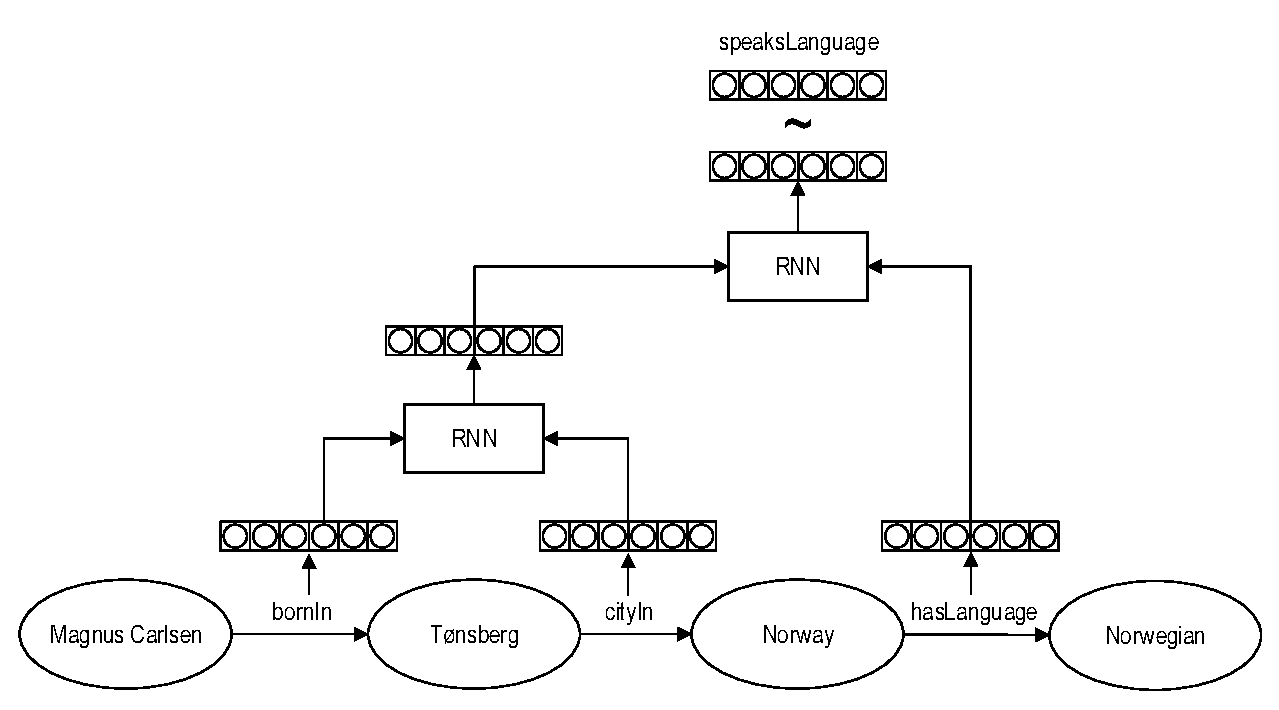
\includegraphics[width=\textwidth]{fig/paths/pathrnn}
%     \caption{Overview of the PATH-RNN method}
%     \label{fig:path-rnn}
% \end{figure}

% \citet{das2017} improve the previously discussed PATH-RNN method with their Single-Model proposal. They point out that taking the embeddings of the entities in a path into account can provide useful information. To represent a path, they recursively combine the embeddings of both the entities and relations in it using RNNs. Furthermore, they propose using a number of different functions to select the best path: \textit{Top-K}, \textit{Average} and \textit{LogSumExp}. They experimentally conclude that the \textit{LogSumExp} function performs better when completing a Knowledge Graph. Figure~\ref{fig:path-single} displays a visual overview of Single-Model. In this Figure, entity embeddings are represented in blue, and relation embeddings in orange. The path that is being considered is the same as in Figure~\ref{fig:path-rnn}.

% \begin{figure}[!htp]
%     \centering
%     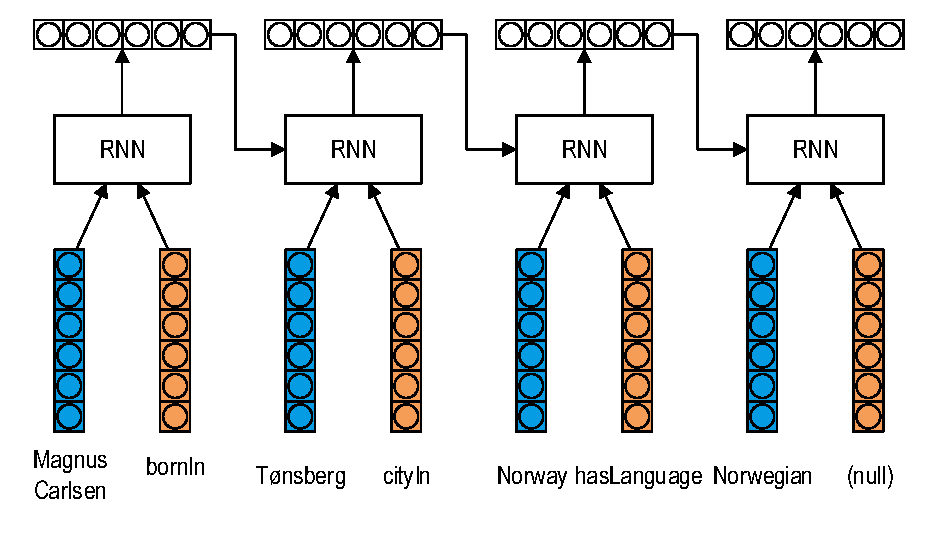
\includegraphics[width=.9\textwidth]{fig/paths/singlemodel}
%     \caption{Overview of the Single-Model method}
%     \label{fig:path-single}
% \end{figure}

% \citet{xiong2018} proposed GMatching, a technique that specializes in extracting information from KG neighborhoods using relatively infrequent relations, which are traditionally considered more challenging due to the reduced amount of information about them present in the graph. GMatching is comprised of two main components: a neighbor encoder, which creates an embedded representation for an entity in a neighborhood; and a matching checker, which computes the similarity of two entity embeddings created by the first component. A visual representation of this proposal is provided in Figure~\ref{fig:path-gmatching}. The meaning of the colors is the same as in the previous Figure.

% \begin{figure}[!htp]
%     \centering
    
%     \subfigure[An example KG]{
%         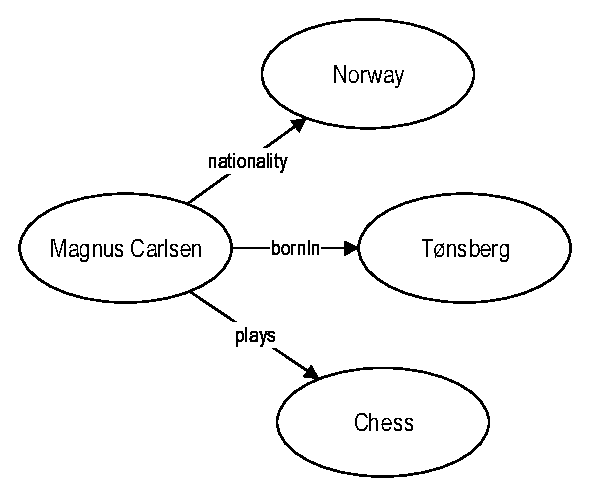
\includegraphics[width=.45\textwidth]{fig/paths/gmatching-a}
%     }\\
%     \subfigure[Encoding of the neighborhood of the entity \textit{Magnus Carlsen}]{
%         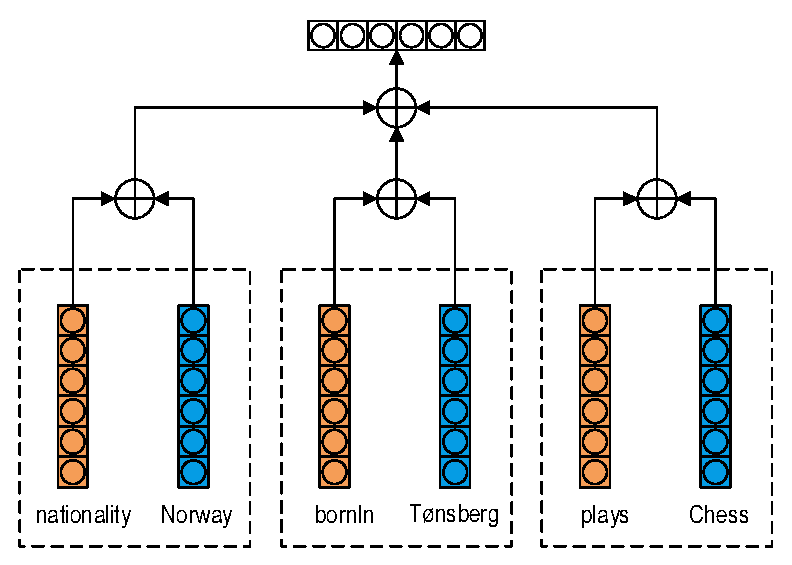
\includegraphics[width=.7\textwidth]{fig/paths/gmatching-b}
%     }

%     \caption{Overview of the GMatching method}
%     \label{fig:path-gmatching}
% \end{figure}

% \citet{shen2017} proposed Implicit ReasoNets (IRNs), a neural network architecture that is able to reason about paths of different lengths in a KG. It is an encoder-decoder model that is governed by a central controller, which allows the whole process to be carried out with no human intervention. Also, it introduces the usage of a shared memory that implicitly stores relevant information about the graph, allowing it to be more efficient and have a smaller memory footprint.

% Additionally, a number of improvements have been made to the baseline translational models to help them leverage path information in several ways. For instance, \citet{lin2015} have proposed PTransE, an extension of TransE that uses path information in its confidence function. Its goal is to give a higher confidence score to those entities that are well-connected together by means of paths that are semantically similar to the relation in the triple that is being evaluated.

% \citet{garcia-duran2015b} proposed RTransE, which represents paths as a series of translations in the embedded space defined by the TransE model. For efficiency reasons, RTransE is limited to using only paths that contain two relations. Likewise, \citet{xiong2018b} introduced PTransD, an enhancement of TransD that performs subsequent translations to model paths. However, PTransD uses two embeddings to represent each entity, to perform operations in parallel.

\section{Summary}\label{sec:path-summary}
The contents of this chapter have provided an overview of the methods to perform Knowledge Graph completion that use relational paths. We have first listed the most prominent scientific proposals that extract paths from a KG and characterize them using features, to learn which paths can be predictive of correct knowledge. Afterwards, we have centered on the proposals that use entity neighborhood information in a number of ways. Finally, we have introduced the approaches that merge together path-based information with latent entity representations, entity and relation embeddings, and neural networks.
    \chapter{Rule-based approaches}\label{chap:rules}

\chapterQuote{\textit{``Logic, like whiskey, loses its beneficial effect when taken in too large quantities.''}}{--- Edward J. M. D. Plunkett, Lord Dunsany}

\chapterAbstract{L}{ogical rules are commonly used to perform Knowledge Graph completion. The proposals that employ these kinds of rules usually mine them first using the triples present in the graph, to generalize specific knowledge stored in it. Then, the extracted rules are used to materialize knowledge in the form of new triples, which can be added back to the KG. In this chapter, we provide an overview of the various ways in which this has been carried out by previous works. It is organized as follows: Section~\ref{sec:rule-intro} lays out the foundational concepts, Section~\ref{sec:rule-ilp} presents the existing methods for mining logical rules from a Knowledge Graph, Section~\ref{sec:rule-cands} introduces the proposals that aim to reduce a set of possible candidate triple using rules, Section~\ref{sec:rule-hybrid} enumerates the approaches that combine rules with other popular ways to complete KGs, and Section~\ref{sec:rule-summary} concludes the chapter.}

\section{Introduction}\label{sec:rule-intro}
Knowledge Graphs are essentially large and incomplete collections of facts about a certain domain. One possible way to complete them is to observe which facts occur frequently together, and then express this relationship as a rule for those combinations that are observed very often. For example, if a person was born, studied and died in a city, it is very likely that they hold the nationality of the country in which that city is located. More formally, this can be expressed through the following logical rule, where $p$ is a person, $c$ is a city, and $C$ is a country:

\[
bornIn(p, c) \wedge studiedIn(p, c) \wedge diedIn(p, c) \wedge cityIn(c, C) \rightarrow hasNationality(p, C)
\]

These rules are called first-order rules, and they represent explicit knowledge, easy for humans to understand and reason about, in opposition to most latent representation models. They are composed of two elements: the body of the rule (left-hand part) represents the logical condition that must be met, and the head (right-hand part) is the knowledge that is considered to be true if the condition is also true.

To complete a Knowledge Graph, one can first extract such rules from it, by observing common appearances of these kind of patterns. Then, the rules can be applied to materialize the head of a rule whenever its body exists, generating new explicit knowledge \cite{stepanova2018}. This process is visually depicted in Figure~\ref{fig:rule-process}.

\begin{figure}[!htp]
    \centering
    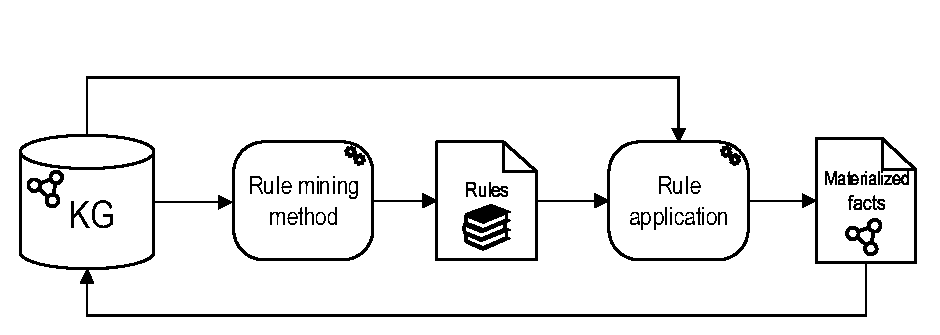
\includegraphics[width=.85\textwidth]{fig/rules/rule_process}
    \caption{Extracting and applying rules on a Knowledge Graph}
    \label{fig:rule-process}
\end{figure}

In this chapter, we present the existing methods in the literature for obtaining and applying first-order rules to complete a Knowledge Graph. First, we introduce the methods that focus solely on rule extraction. Then, we present some applications of first-order rules to the task of candidate filtering. Finally, we discuss some proposals that combine rules with other ideas presented in previous chapters.

\section{Rule mining methods}\label{sec:rule-ilp}
There are a number of approaches to mine first-order rules in Knowledge Graphs. One of them is using Inductive Logic Programming (ILP) \cite{muggleton1994}, a classical statistical relational learning method that can be used to extract such rules from a collection of facts.

In this regard, \citet{jiang2016} have proposed using ILP to perform Knowledge Graph completion on KGs that have a strong time constraint component. Such a KG may contain information on whether a person is the president of a country, whose correctness depends on the time period in which it is interpreted. In this proposal, the most common time periods for an assortment of different facts are inferred through ILP, and then used to assess the correctness of future facts. However, it relies on all facts having time annotations, which may not be commonplace.

\citet{galarraga2015} proposed the AMIE+ method, which generates similar rules using ILP. AMIE+ addresses the fact that, due to the Open World Assumption (OWA), a fact that is not present in a KG should not be considered false, but instead simply unknown. The OWA thus makes it very challenging to generate truly false examples to assess the overall validity of a rule. The authors use a bespoke confidence measure for their rules, known as the partial completeness assumption confidence. AMIE+ improves the efficiency of its predecessor method AMIE \cite{galarraga2013} and can be applied to larger Knowledge Graphs.

\citet{wang2015} refine this idea with their RDF2Rules method. Contrary to AMIE+, which is limited to only being able to mine one rule at a time, RDF2Rules speeds up the process by parallelizing rule extraction. It achieves this by detecting and extracting frequent relation cycles of a certain length in a KG, which are essentially loops that contain a given amount of relations. An example of such a loop can be found in Figure~\ref{fig:rule-cycle}. Note that the directionality of the edges in a KG is relevant for the existence of a cycle. Once the most common cycles have been obtained, a number of rules can be extracted from them. This is done by iteratively selecting one relation as the head of the rule and the rest as the body, advancing on the loop, and repeating this process until the entire loop has been traversed.

\begin{figure}[!htp]
    \centering
    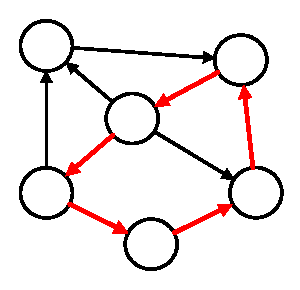
\includegraphics[width=.35\textwidth]{fig/rules/cycle}
    \caption{A cycle of 5 relations in a sample Knowledge Graph}
    \label{fig:rule-cycle}
\end{figure}

The Never-Ending Language Learning (NELL) system that was proposed by \citet{mitchell2018} also learns knowledge rules from the data that it is constantly provided. These rules are manually screened to ensure a high level of quality, so as to not introduce incorrect facts into a Knowledge Graph. It then applies these rules to generate knowledge that was previously missing.

Markov Logic Networks (MLNs) \cite{richardson2006} have also been used for the task of completing a Knowledge Graph. MLNs combine the previously discussed rules with probabilistic models, which allows them to derive generalized knowledge from a smaller corpus of facts and to better handle complex and noisy information \cite{yang2017}.

The use of MLNs for Knowledge Graph completion has been analyzed by \citet{kuzelka2019}. The authors conclude that MLNs can provide a satisfactory performance on this task, assuming that the triples that are missing from the graph are independent from one another and have a roughly equal probability of being true, which is not always the case \cite{borrego2019}.

\citet{yang2017} presented Neural Logic Programming (NeuralLP), an approach that combines first-order rule mining with sparse matrix multiplication. In this approach, the authors propose using an attention mechanism to further refine the confidence value that is assigned to each individual triple. The main rule mining mechanism in NeuralLP is governed by a central neural controller. Additionally, it is able to learn rules of variable length with more ease than its predecessors.

Furthermore, \citet{sadeghian2019} introduced DRUM, which extends NeuralLP by analyzing the structure and confidence values of the rules that are being inferred, and then approximating these elements for other rules using tensors. It, however, is only limited to positive examples due to the OWA and is not able to infer negative rules. 

\citet{rocktaschel2017} proposed NTP, a similar method to NeuralLP, which infers rules by using transitive relations between facts. Their approach requires that such relations be represented as a vector or a tensor, in order to leverage the semantic similarities that are commonly exploited in embedded spaces. It nonetheless suffers from a lesser scalability than the original NeuralLP method, due to the computational complexity that is required to carry out the process of rule inference.

To address the aforementioned scalability issues, \citet{minervini2018} presented an improved NTP2.0 method. This new version is able to focus only on the most promising rules during the mining process, by using a pooling method that is able to monitor the creation of multiple rules at once.

\section{Candidate filtering}\label{sec:rule-cands}
Some authors have proposed rule-based techniques for filtering candidate triples, instead of generating new knowledge. The process of generating and applying these rules is fundamentally different: due to the very large number of possible candidate triples, the rules must not be computationally expensive to apply. Additionally, it is not as important for them to be fully correct, since an incorrect fact will be evaluated in more detail further down the KG completion process. It is, however, desirable that the candidate filtering rules exclude as few correct candidates as possible, in order not to hinder the quality of the final set of generated triples.

\citet{wei2015} proposed the INS method, which uses the previously discussed TransE embedding model to filter out possibly incorrect knowledge. More specifically, they employ TransE to analyze the semantic similarity between the two entities in a triple, and discard the triple if the similarity does not exceed a certain threshold. This results in sets of candidate triples that are smaller than the original ones.

\citet{shi18} also argued that it is generally not practical to apply any model to the whole set of possible candidate triples, and that it must be narrowed down in some way. In their work, they use a set of simple rules to determine that any given triple $(s, r, t)$ is a valid candidate if another triple with the structure $(\_, r, t)$ is already present in the Knowledge Graph.

\citet{zhang2019} proposed IterE, an approach that prunes knowledge using graph traversing and random selection. It generates a set of plausible rules and monitors their performance as they are being built, removing those that are found not satisfactory and leaving only a smaller set of rules that can be generated quickly.

Some of the previously discussed works can also be used for filtering candidate triples. The authors of NTP2.0 \cite{minervini2018} proved that a k-nearest neighbor search can provide satisfactory results to filter out wrong knowledge when inferring rules, which can be performed efficiently.

Other proposals incorporate parameters that can be fine-tuned to rapidly rule out rules that are not satisfactory. \citet{omran2018} proposed RLvLR, which allows the user to set values for the minimum required confidence for a rule. A similar approach is followed by the already discussed DRUM \cite{sadeghian2019} method.

Additionally, the AMIE+ method \cite{galarraga2015} can also be used for this purpose. It includes a number of strategies that can be used to prune a set of candidate triples, by producing simpler rules with a high support. Additionally, AMIE+ can perform confidence approximations, which allows it to speed up the rule inference process, making it more appealing for its application to candidate filtering.


\section{Hybrid approaches}\label{sec:rule-hybrid}
Even though rule-based approaches excel in their explainability, they often have trouble scaling up to very large Knowledge Graphs \cite{shen2022overview}. To overcome this issue, many authors have proposed methods that combine more traditional rule mining with other approaches discussed in previous chapters, to try to guide the rule mining process towards more promising rules.

One of the first such proposals was made by \citet{wang2015b}, who introduced the r-KGE method. It combines the tensor-based model RESCAL, the embedding-based model TransE, and logical rules. These rules are then used to prune the embedded space using integer linear programming \cite{schrijver1999}, which sees a significant reduction of its size. However, it is not properly equipped to handle N-to-N relations, and its reasoning process can still be quite computationally expensive. The overall model proposed by r-KGE is shown in Figure~\ref{fig:rule-rkge}.

\begin{figure}[!htp]
    \centering
    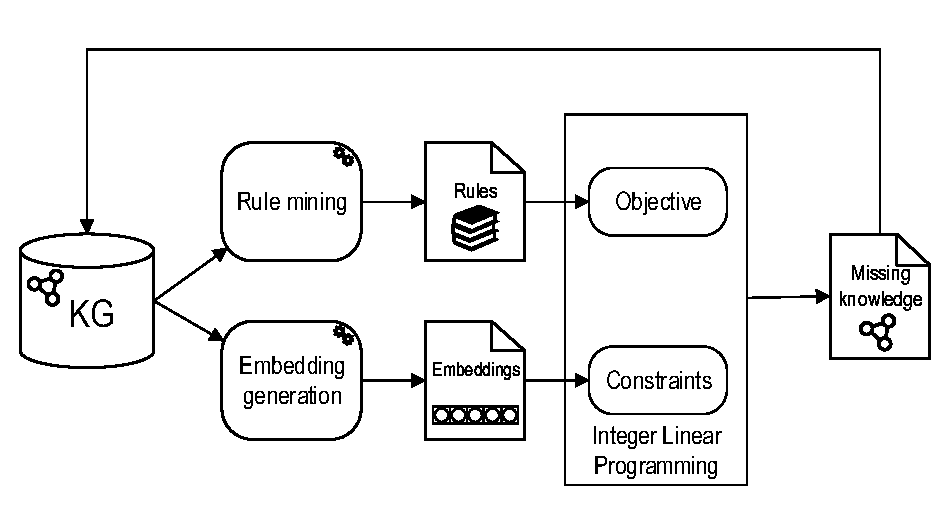
\includegraphics[width=.9\textwidth]{fig/rules/rkge}
    \caption{Overview of the r-KGE model}
    \label{fig:rule-rkge}
\end{figure}

The previously discussed INS method \cite{wei2015} also incorporates TransE to quickly compute the degree of similarity between entities, and limits the rule reasoning process by taking only the top N most similar entities into consideration. Additionally, this similarity score can provide an approximation of the quality of a rule before it is completely built.

\citet{guo2016} introduced KALE, another model that combines logical rules and entity embeddings. KALE aims to provide a common ground in which rules and embeddings can directly interact, by representing triples as atomic formulae and rules as combination of these formulae. The semantic similarity information that is intrinsically present in the entity embeddings aids in expanding the predictive capabilities of the rules and their generality. A visual overview of the KALE architecture is provided in Figure~\ref{fig:rule-kale}. In this Figure, entity embeddings are represented in blue, relation embeddings in orange, and scalar confidence values in green.

\begin{figure}[!htp]
    \centering
    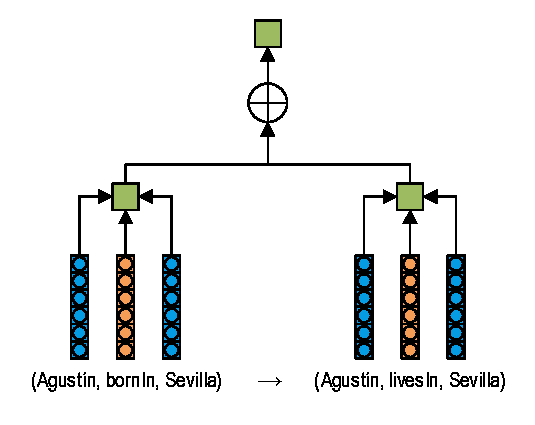
\includegraphics[width=.65\textwidth]{fig/rules/kale}
    \caption{Overview of the KALE model}
    \label{fig:rule-kale}
\end{figure}

The same authors \cite{guo2018} also presented RUGE, a KG completion technique that combines the same elements in an iterative fashion. Rather than relying on pre-computed entity embeddings, RUGE generates its own embedded space with the aid of logical rules. Additionally, RUGE is able to operate on Knowledge Graphs that has both labeled and unlabeled triples. A series of logical rules are applied on the unlabeled triples to label them. Then, the labeled triples are used to rectify and improve the embedded space so that it better captures the relations between the entities. The improved embedded space provides feedback on the labels, and the rules can be updated accordingly. A diagram depicting this process can be found in Figure~\ref{fig:rule-ruge}.

\begin{figure}[!htp]
    \centering
    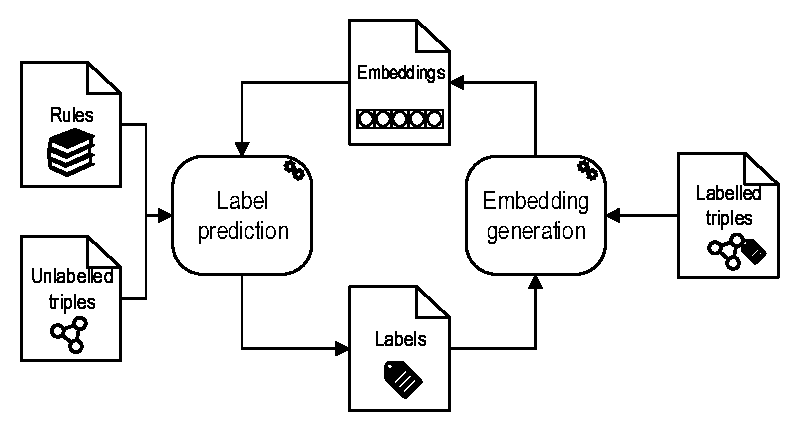
\includegraphics[width=.85\textwidth]{fig/rules/ruge}
    \caption{Overview of the RUGE model}
    \label{fig:rule-ruge}
\end{figure}

Furthermore, another aforementioned method, IterE \cite{zhang2019}, proposes a similar approach. IterE generates an initial set of entity embeddings for the Knowledge Graph. These embeddings are used to generate a set of rules, whose quality is evaluated. The best-performing rules are then used to generate new triples that are introduced in the KG, and the process starts anew by generating new embeddings that take into account the newly generated knowledge. This is shown in a graphical manner in Figure~\ref{fig:rule-itere}.

\begin{figure}[!htp]
    \centering
    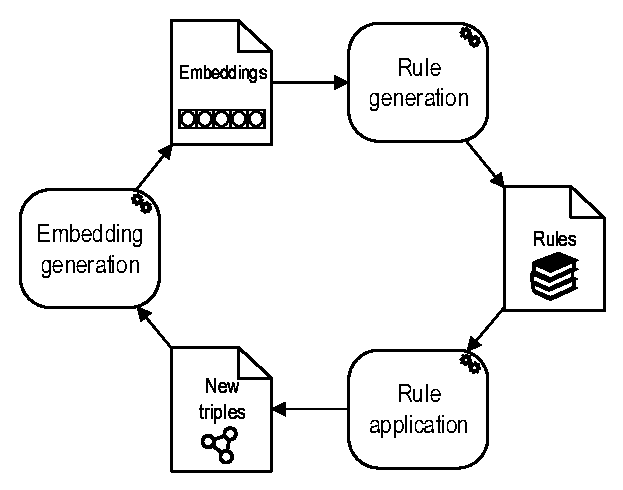
\includegraphics[width=.65\textwidth]{fig/rules/itere}
    \caption{Overview of the IterE model}
    \label{fig:rule-itere}
\end{figure}

\citet{meilicke2019} proposed AnyBURL, a technique that can generate logic rules in a bottom-up manner and on-demand. AnyBURL works by deconstructing a Knowledge Graph into a set of labeled paths. Then, it uses path-based features to determine which paths contain more useful information to obtain rules from. AnyBURL is more lightweight than other related rule-based proposals and, due to the fact that it only considers the most promising paths inside a KG, can be applied to larger graphs.

\citet{niu2020} presented RPJE, a proposal that brings together path-based information and first-order rules. It first mines logical rules, and then uses those of length 2 to combine paths in the KG, and rules of length 1 to create a number of semantic relations.

Finally, \citet{ma2019} introduced ELPKG, a proposal that brings together all three main approaches that we have covered in the previous chapters. It uses entity embeddings to represent the relations between entities, and a breadth-first search to detect the paths between the two entities in a triple. The information gained from both the embeddings and the paths is combined together, and it then applies soft logic to obtain the final confidence value for the triple. 

\section{Summary}\label{sec:rule-summary}
This chapter has provided an overview of the current approaches to Knowledge Graph completion that are based on logical rules. First, we have introduced the proposals that can be found in the literature that rely solely on obtaining and applying these rules. Then, we have focused on the methods for filtering candidate triples using first-order rules. At last, we covered the methods that combine rule mining with path-based information or latent representations, such as tensors or entity embeddings.

    %%%%%%%%%%%%%%%%%%%%%%%%%%%%%%%%%%%%%%%%

    \part{Our Proposal}
    \chapter{SpaceRL framework}\label{chap:framework}

\chapterQuote{\textit{``Most problems can be solved using algebra, or violence.''}}{--- Bill Wurtz}

\chapterAbstract{B}{efore we delve into the details of our proposal, it is important to establish a common and unambiguous vocabulary. For this reason, we have devised a conceptual framework that allows us to describe a number of relevant concepts in detail. The chapter is organized as follows: Section \ref{sec:theo-intro} introduces it, Section \ref{sec:theo-triple} models the concept of a triple, Section \ref{sec:theo-kg} presents the theoretical model of a Knowledge Graph, Section \ref{sec:theo-paths} introduces topology-based elements such as paths, distances and reachability, Section \ref{sec:theo-subgraph} illustrates the concept of neighborhood subgraphs, Section \ref{sec:theo-candidates} presents the notions of candidate triples and candidate-filtering fitness, Section \ref{sec:theo-rule} describes candidate-filtering criteria and rules, and Section \ref{sec:theo-features} introduces graph-based features and feature groups; finally, Section \ref{sec:theo-conclusion} summarizes the chapter.}

\section{Introduction}\label{sec:theo-intro}
% Throughout our proposal, we use a number of concepts, both established in this field and novel. In this chapter, we define their foundations, such as tuples of entities and relations known as triples, or the fields of a Knowledge Graph, which allow us to accurately describe further concepts. We also define paths inside a Knowledge Graph, which are the basis for many of the elements in our proposal. Building upon the notion of a path, we provide a formal definition of the distance between two entities in a Knowledge Graph, as well as of the concept of entity reachability.

% Furthermore, in this chapter, we define neighborhood subgraphs, which are portions of a KG that contain the elements most closely related to a given entity. Then, we introduce candidate triples, which are combinations of entities and relations that have a high likelihood of representing correct knowledge. To measure the tentative aptness of a candidate triple, we present the idea of candidate fitness. In order to rule out those candidate triples with a low fitness, we define candidate filtering criteria and rules. Finally, we introduce a way to numerically model a triple in a KG through the use of graph-based feature groups.

% \begin{figure}[htp]
%     \centering
%     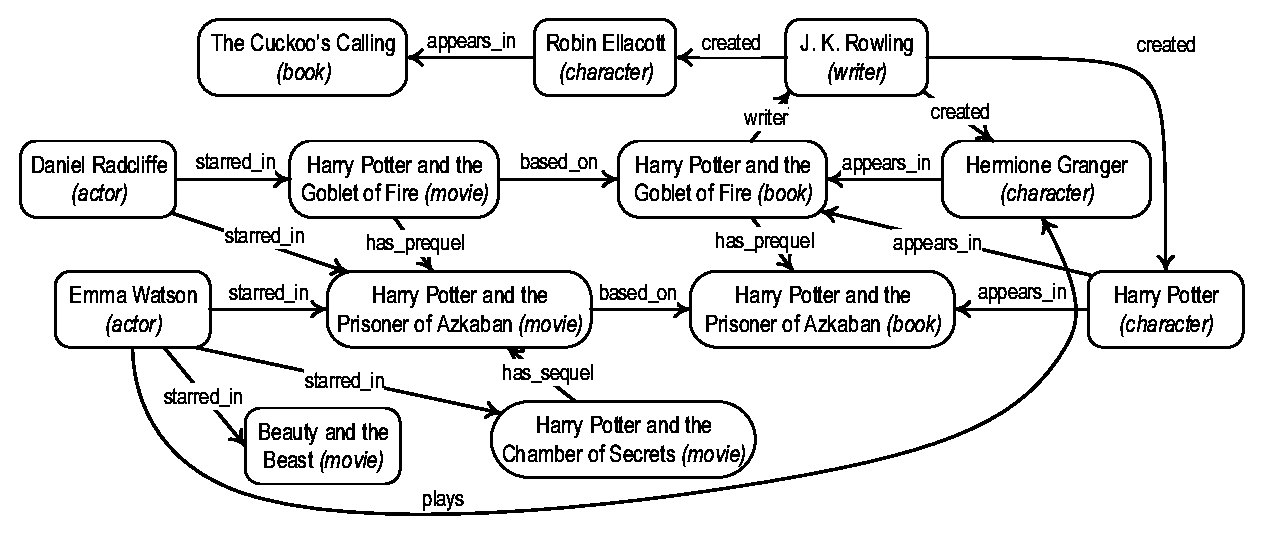
\includegraphics[width=\textwidth]{fig/theoretical/kg-harry-potter}
%     \caption{Sample KG describing works, actors, writers and characters}
%     \label{fig:kg-potter}
% \end{figure}

% To help illustrate some concepts in this chapter, Figure~\ref{fig:kg-potter} presents a KG that contains information about fictional works, actors, writers and characters.

\section{Triple}\label{sec:theo-triple}
% The notion of a triple is pivotal to Knowledge Graphs, since it constitutes an atomical amount of structured information. A triple is a 3-tuple that contains two entities, commonly denoted \textit{source} and \textit{target}\footnote{Other literature sometimes refers to the two entities in a triple as \textit{head} and \textit{tail} \cite{dessi2022cskg,dessi2020aikg,bordes2013}, or \textit{subject} and \textit{object} \cite{nickel2016, balazevic2019,trouillon2016}.}; connected by means of a relation. This, in turn, represents a fact in a given domain.

% Formally, a triple is defined as follows:

% \defin{Triple}{
%     Let \Eset{} be a set of entities, and let \Rset{} be a set of relations. We define a triple as a 3-tuple that represents the existence of a relation $r \in \Rset$ between a source entity $s \in \Eset$ and a target entity $t \in \Eset$. We denote triples as \triple.
% }

% In the sample KG depicted in Figure \ref{fig:kg-potter}, a sample triple is \tripleSty{(Emma Watson, starred\_in, Beauty and the Beast)}.

%Furthermore, a triple only represents positive knowledge...

\section{Knowledge Graph}\label{sec:theo-kg}
% A collection of triples forms a Knowledge Graph, which contains an assorted set of facts. Although, as discussed, triples have no inherent guarantees about the correctness of the knowledge they represent, it is in the best interests of both the curators and users of Knowledge Graphs to ensure that the triples contained in it are as trustworthy as possible.

% A Knowledge Graph can thus be defined as:

% \defin{Knowledge Graph}{
%     Let \Eset{} be a set of entities, let \Rset{} be a set of relations, and let \Tset{} be a set of triples of the form $\{\triple \mid s, t \in \Eset, r \in \Rset\}$. We define a Knowledge Graph as $\KG = (\Eset{}$, $\Rset{}$, $\Tset{})$.
% }

% It is important to note that, in addition to a set of triples, KGs also contain the sets of entities and relations, \Eset{} and \Rset{} respectively, that are considered to be included in the KG and thus allowed to take part in the triples that compose the KG. Although this may seem limiting, they are routinely expanded as new knowledge is added to a KG~\cite{dong2014}.

% Figure \ref{fig:kg-potter} graphically represents a KG with 13 entities, 7 distinct relations and 19 triples, represented as edges that connect pairs of entities.

% Note that a triple in a Knowledge Graph states a fact, but it may be one that is not considered to be true or correct. We thus define a correct triple as follows:

% \defin{Correct triple}{
%     Let $\KG = \KGlong$ be a Knowledge Graph, and let $\tripleSty{(s, r, t)} \in \Tset$ be a triple in \KG. We consider that the triple is correct if the relation that it establishes between $s$ and $t$ holds true in the real world or in the domain of application of $\KG$.
% }

% For example, the triple \tripleSty{(Barack Obama, born\_in, Kenya)} is formally valid, but it is not correct. It is also noteworthy that the real-world correctness of a triple may depend on the time period in which it is interpreted, for example, \tripleSty{(Barack Obama, president\_of, United States)}. A triple, on its own, does not have a mechanism to express a time constraint or any other restrictions about its correctness.

% \section{Topology-based concepts}\label{sec:theo-paths}
% Since a KG is a specific case of graph, we can leverage some concepts that arise from using such a structure. 

% \subsection{Paths between entities}
% Given two entities in a Knowledge Graph, a relevant question is whether there exists a path in the KG that connects them together. To answer this question, we must first define the concept of path:

% \defin{Path}{
%     Let $\KG = \KGlong$ be a Knowledge Graph, and let $s, t \in \Eset$ be two entities in \KG. We define a path $p$ between $s$ and $t$ as a sequence of triples of the form $p = \langle\,(e_i,\,r_i,\,e_{i+1})\,\rangle$ for $i = 1..n$, where $e_1 = s$, $e_{n+1} = t$ and $(e_i, r_i, e_{i+1}) \in \Tset$ for  $i = 1..n$.  We denote a path $p$ between $s$ and $t$ using the relations $r_1\ldots r_n$ as \kgpath{s}{t}{r_1, r_2, \ldots, r_n}, or \kgpathl{s}{t}{n} for short.
% }

% Building upon the previous definition, to further characterize a path, we define the length of a path as follows:

% \defin{Path length}{
%     Let $s$ and $t$ be two entities in $\KG$ with $s, t \in \KG$. Let $p$ be a path between $s$ and $t$ of the form $p = \langle\,(e_i,\,r_i,\,e_{i+1})\,\rangle$ for $i = 1..n$. We define the length of a path as the number of triples it contains, i.e., $|p|$.
% }

% In the KG depicted in Figure \ref{fig:kg-potter}, an possible example of a path of length 2 between the entities \textit{J.K. Rowling} and \textit{The Cuckoo's Calling} would be $\langle\, \tripleSty{(J.K. Rowling, created, Robin Ellacott)}, \tripleSty{(Robin Ellacott, appears\_in, The Cuckoo's Calling)}\,\rangle$.

% It is possible that there exists more than one possible path between a pair of entities. It is also a possibility that there are no possible paths between two entities. Thus, it can be useful to know how many distinct paths of a given length there exist connecting two given entities. For this purpose, we define a set of possible paths as follows:

% \defin{Possible paths}{
%     Let $s$ and $t$ be two entities in $\KG$ with $s, t \in \Eset$. We denote the set of all possible distinct paths of the form \kgpath{s}{t}{r_1, r_2, \ldots, r_n} as \kgpathP{s}{t}{r_1, r_2, \ldots, r_n}.
% }

\subsection{Distance between entities}
% In light of the previous definitions, it now seems reasonable to devise a measure of how close two entities are in a given Knowledge Graph. Given that KGs are not weighted graphs, we can define the distance between two entities as the minimum number of relations that we have to traverse to go from the first one to the second. Formally, the distance is defined as follows:

% \defin{Distance between entities}{
%     Let $\KG =$ $\KGlong$ be a Knowledge Graph, and let $s, t \in \Eset$ be two entities in \KG. We define the distance between $s$ and $t$ as the length of the shortest path that exists between $s$ and $t$ in \KG, i.e., $|\kgpathl{s}{t}{n}|$ such that $\nexists~\kgpathl{s}{t}{i} \mid i < n$.
%     If no path of any length exists between $s$ and $t$, then the distance between them is $\infty$.
%     We denote the distance between $s$ and $t$ in $\KG$ as $dist(\KG, s, t)$.
% }

% In the KG depicted in Figure \ref{fig:kg-potter}, the distance between the entities \textit{Daniel Radcliffe} and \textit{Harry Potter} is 4, since that is the length of the shortest path that exists between them. 

% The careful reader will note that, due to the fact that KGs are directed, distance is not symmetric, and thus the order of the entities is relevant: the distance between \textit{Harry Potter} and \textit{Daniel Radcliffe} in Figure \ref{fig:kg-potter} is $\infty$ because no path exists between them. The impossibility of such a path can be trivially verified by noting that \textit{Daniel Radcliffe} has no inbound edges.

\subsection{Reachability}
% Most graph algorithms rely on some notion of whether an entity is reachable from another one or not, and expand upon this notion to build assessments about the whole graph, for example, by determining its connected components. Knowledge Graphs are no exception, but given the semantical differences of the relations in them, it makes sense to restrict this notion of reachability to be able to answer a more precise question: ``\textit{Is an entity reachable from another one through a certain relation?}''

% To formalize this idea, we define reachability in a KG as follows:

% \defin{Reachability}{
%     Let $\KG = \KGlong$ be a Knowledge Graph, let $s, t \in \Eset$ be two entities in \KG, let $r \in \Rset$ be a relation in \KG, and let $n \ge 1$ be a natural number. We define Reach as a predicate that determines whether there exists a path of length $n$ between $s$ and $t$ in \KG{} such that the relation $r$ appears in the last triple of the path, i.e., $Reach(\KG,$ $s$, $t$, $r$, $n)$ $\Longleftrightarrow$ $\exists~ \kgpathl{s}{t}{n} \land \exists~ a \in \Eset{} \mid$ $last(\kgpathl{s}{t}{n}) = (a, r, t)$.
% }

% With a reachability predicate, we can proceed to find a subset of entities in a KG that are reachable from a given entity using a certain relation and distance:

% \defin{Reachable entities}{
%     Let $\KG = \KGlong$ be a Knowledge Graph, let $s, t \in \Eset$ be two entities in \KG, let $r \in \Rset$ be a relation in \KG, and let $n \ge 1$ be a natural number. We define the set of entities that can be reached from $s$ through a relation $r$ at distance $n$ as the set of entities that match the predicate Reach under such circumstances, i.e., $\{t \in \Eset$ $\mid Reach(\KG,$ s, t, r, n$)\}$. We denote the previously defined set as $Reachable(s, r, n)$.
% }

% In the example KG depicted in Figure \ref{fig:kg-potter}, $Reachable($\textit{Hermione Granger, writer, 2}$) = \{$\textit{J.K. Rowling}$\}$.

\section{Neighborhood subgraphs}\label{sec:theo-subgraph}
% The previous sections have given us the necessary tools to accurately establish the concept of ``neighborhood'' in a KG by leveraging its topology. It seems appropriate to define that an entity $e_1$ should be in the neighborhood of $e_2$ if $e_1$ is reachable from $e_2$, given the previous definitions\footnote{Again, the non-symmetricality of distance may result in $e_1$ being in the neighborhood of $e_2$, but not vice-versa. Sadly, good neighbors are not always reciprocated.}. Since reachability is constrained by distance and a specific relation, we define the neighborhood subgraph of a given entity as follows:

% \defin{Neighborhood subgraph}{
%     Let $\KG = \KGlong$ be a Knowledge Graph, let $e \in \Eset$ be an entity in \KG, and let $n \ge 1$ be a natural number. We define the neighborhood subgraph of $e$ of size $n$ as a Knowledge Graph $\subKGdef = (\Eset{}_e^n$, $\Rset{}$, $\Tset{}_e^n)$ that contains the triples whose target entities can be reached from $e$ at a distance of at most $n$ through any relation, and the entity set that can be derived from such triples, where $\Tset{}_e^n$ $=$ $\{(s', r', t') \in \Tset \mid Reach(\KG$, e, $t'$, $r'$, i$),~$i = 1..n$\}$ and $\Eset{}_e^n = $ $\bigcup\{\{s, t\} \subseteq \Eset{} \mid (s, r, t) \in \Tset{}_e^n\}$.
% }

% To help illustrate this concept, Figure \ref{fig:context-examples} showcases two possible neighborhood subgraphs for the KG shown in Figure \ref{fig:kg-potter}.

% \begin{figure}[htp]
%     \begin{center}
%         \def\subfigwidth{.6\textwidth}
%         \subfigure[Neighborhood subgraph of size 2 for the entity \textit{Daniel Radcliffe}]{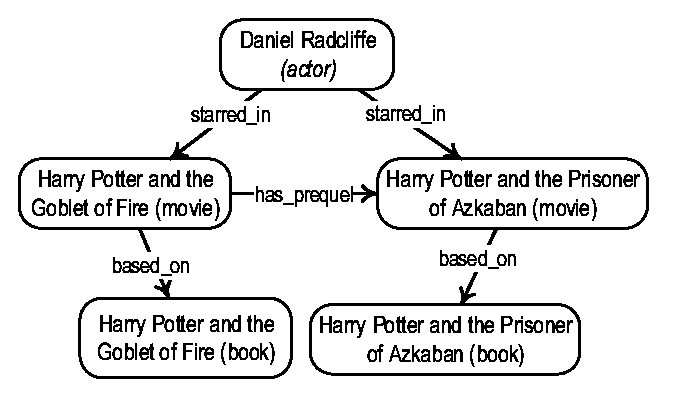
\includegraphics[width=\subfigwidth]{fig/theoretical/example_subgraph_1}\label{fig:context-examples-a}}\\
%         \subfigure[Neighborhood subgraph of size 3 for the entity \textit{Harry Potter}]{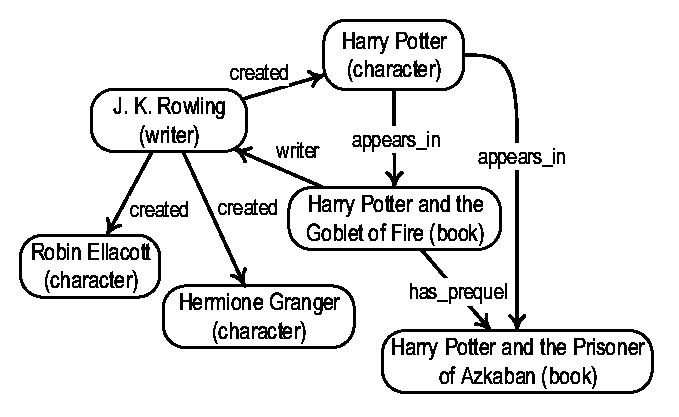
\includegraphics[width=\subfigwidth]{fig/theoretical/example_subgraph_2}\label{fig:context-examples-b}}
%         \caption{Two neighborhood subgraphs for the KG shown in Figure \ref{fig:kg-potter}}
%         \label{fig:context-examples}
%     \end{center}
% \end{figure}

\section{Candidates}\label{sec:theo-candidates}
% As discussed earlier, triples do not make inherent guarantees about the correctness of the knowledge they represent. To represent triples with a higher knowledge quality, this section introduces candidate triples and the notion of fitness in candidate filtering.

\subsection{Candidate triples}
% One can form a syntactically correct triple by just combining two random entities with a random relation. However, chances are that the resulting fact is most likely not correct. Contrary to such a low-quality triple, a candidate triple, or just ``candidate'' for short, is a triple that has been created in such a way that its chance to represent correct knowledge is significantly higher than by mere randomness:

% \defin{Candidate}{
%     Let $\KG = \KGlong$ be a Knowledge Graph, let $s, t \in \Eset$ be two entities and let $r \in \Rset$ be a relation in \KG. We define a candidate as a triple $(s, r, t)$ that has a significantly high chance to represent real-world knowledge, even if it does not exist in \Tset.
% }

% For example, given the KG shown in Figure \ref{fig:kg-potter}, a candidate triple could be \tripleSty{(Daniel Radcliffe, plays, Harry Potter)}. Note that this triple does not exist in the KG in its current state.

\subsection{Fitness function}
% Candidate triples can be generated in a wide manner of ways, that we discuss in more detail in the following chapter. However, it is clear that the number of possible triples, in terms of combinations of entities and relations, is generally orders of magnitude greater than the amount of triples present in any given KG. Therefore, it is possible to generate very large sets of candidate triples that are not yet in a KG.

% As a consequence, it is generally desirable to reduce these sets of candidate triples in a manner that maximizes the preservation of triples with a higher chance to be correct~\cite{shen2022overview, borrego2019}. To formalize this idea, we introduce the concept of fitness function, which assesses the quality of a set of candidate triples in terms of its size and how many correct triples it contains.

% \defin{Fitness function}{
%     Let $\KG =$ $\KGlong$ be a Knowledge Graph, let \Sset{} be a set of candidates and let $\Sset'$ be a set of filtered candidates, with $\Sset' \subseteq \Sset$. We define fitness as a function $fitness(\KG, \Sset, \Sset') \rightarrow \mathbb{R}$ that assigns a score to the filtered set of candidates, with respect to the original set of candidates and KG.
% }

% Since there are many ways to achieve this, we introduce specific instances of fitness functions in the context of KG completion in Chapter~\ref{chap:chai}.

\section{Candidate filtering}\label{sec:theo-rule}
% As previously discussed, it is generally necessary to reduce the size of a set of candidate triples, in order to better assess the remaining candidates for their inclusion in a KG. To achieve this, this section introduces the concept of criterion, and then builds upon it to present the definition of a candidate-filtering rule.

\subsection{Criterion}
% A criterion is an atomic element in candidate filtering. Given a candidate triple in the context of a particular Knowledge Graph, a criterion assigns a binary \texttt{False/True} label to the candidate, denoting whether it should be discarded immediately (\texttt{False}), or tentatively accepted and evaluated more carefully (\texttt{True}):

% \defin{Criterion}{
%     Let $\KG =$ $\KGlong$ be a Knowledge Graph and let the triple $T = (s, r, t)$ be a candidate for $\KG$. We define a criterion as a function $cr(\KG, T) \rightarrow \{False, True\}$ that assigns a binary label to a candidate triple in the context of a KG.
% }

% A given criterion defines a certain method to determine if a candidate triple is likely to be correct or not. For example, a possible criterion would be to accept all candidate triples in which the distance between its two entities is lower than a threshold.

\subsection{Rule}
% In order to express more complex manners of filtering candidate triples, we combine several criteria into a rule. A candidate-filtering rule also produces a binary output for a candidate, in this case, by evaluating multiple criteria and combining their results using conjunctions and disjunctions:

% \defin{Rule}{
%     Let $\KG =$ $\KGlong$ be a Knowledge Graph, let the triple $T = (s, r, t)$ be a candidate for $\KG$, and let $cr_1,\,cr_2,\,\ldots,\,cr_n$ be a number of criteria. We define a rule as a function $rule(\KG, T) \rightarrow \{False, True\}$ resulting of the conjunction and/or disjunction of several criteria, i.e., $cr_1\,(\wedge | \vee)\,cr_2\,(\wedge | \vee)\,\dots (\wedge | \vee)\,cr_n$.

% }

\section{Graph-based features}\label{sec:theo-features}
% To numerically characterize a triple, we propose a set of graph-based features that takes neighborhood subgraphs, reachable entities and paths into account. Due to the possibly large number of different features that can exist, we also introduce the concept of feature groups. Each group can be parameterized to obtain a specific feature, which we call an instance of the feature group.

\subsection{Feature}
% A feature is the simplest way to characterize a triple in the context of the Knowledge Graph it belongs to, by assigning a real number to it according to some operation:

% \defin{Feature}{
%     Let $\KG = \KGlong$ be a Knowledge Graph. We define a feature $f$ as a function $f : \Tset \rightarrow \mathbb{R}$ that assigns a real number to a triple.
% }

% For example, a feature $f$ may convert a triple into the number of entities in the neighborhood subgraph of size 2 of the source entity, i.e., $f : \triple \mapsto |\Eset{}_s^2|$.

\subsection{Feature group}
% Features can have an infinite number of small variations. In our previous example, we mentioned that a feature may leverage the neighborhood subgraph of size 2, but one may conceivably use any subgraph size that is considered appropriate. To be able to express these variations in a more concise way, we define a feature group as follows:

% \defin{Feature group}{
%     Let $\KG = \KGlong$ be a Knowledge Graph. We define a feature group $f_n$ as a function $f_n : \fancy{X} \rightarrow (\Tset \rightarrow \mathbb{R})$ that receives a set of parameters \fancy{X} and returns a feature.
% }

% % TODO: newpage?
% For example, a feature group $f_0$ may return a feature that converts a triple into the number of entities in the neighborhood subgraph of size $n$ of the source entity, i.e., $f_0(n) = f : \triple \mapsto |\Eset{}_s^n|$, where $n$ is a parameter of the feature group. Thus, $f_0(2) : \triple \mapsto |\Eset{}_s^2|$, which is the feature shown in the previous example. Consequently, feature groups allow us to represent a set of very similar features in a more compact way, where the only distinction between said features is a given set of parameters.

\section{Summary}\label{sec:theo-conclusion}
In this chapter, we have described the conceptual framework our proposal relies on. We have defined Knowledge Graphs, triples, paths, distance in a KG and reachability. Furthermore, we have introduced neighborhood subgraphs, candidate triples and fitness functions, as well as candidate-filtering criteria and rules. Finally, we have described graph-based features and their groups.
    \chapter{CHAI: Our candidate filtering proposal}\label{chap:chai}

\chapterQuote{\textit{``I say let the world go to hell, but I should always have my tea.''}}{--- \textit{Notes from Underground}, Fyodor Dostoyevsky}

\chapterAbstract{T}{he first step towards completing a Knowledge Graph is narrowing down an initial set of theoretically potential candidates into a smaller subset that still retains most of the promising ones. This chapter introduces CHAI, our proposal for filtering candidate triples, and it is structured as follows: Section~\ref{sec:chai-intro} introduces the chapter, Section~\ref{sec:chai-proposal} explains the criteria that CHAI uses, as well as the algorithm that it follows to create rules from them, Section~\ref{sec:chai-architecture} discusses its software architecture, Section~\ref{sec:chai-evaluation} presents our experimental validation of CHAI and the conclusions we draw from it, Section~\ref{sec:chai-limitations} delves into the practical limitations of CHAI, and Section~\ref{sec:chai-summary} concludes the chapter.}

\section{Introduction}\label{sec:chai-intro}
% In this chapter we introduce CHAI~\cite{borrego2019}, our method for generating rules that are able to filter candidate triples in the context of a KG completion process by combining a number of criteria in such a way that it optimizes a given fitness function. CHAI works by producing rules that can be applied on the initial set of candidates and produce a reduced set that contains only the promising candidate triples. Then, this set can be passed on to any fact checking technique to check the correctness of each promising candidate and identify correct triples that complete the KG. The rules produced by CHAI are based on different criteria that take the internal features of the KG into account, such as the domains and ranges of every relation in the KG, in addition to the distances between its entities.

% Additionally, we evaluate CHAI on a number of different Knowledge Graphs, and we show that it is able to achieve a good performance when dealing with all relationships in every KG under study, demonstrating that it is a generic and effective method, suitable for web-scale contexts.

% Through this chapter, we continue to follow the running example of a Knowledge Graph that was introduced in Section~\ref{sec:theo-intro}.

\section{Our proposal}\label{sec:chai-proposal}
% When completing a Knowledge Graph, there is a very large number of possible triples that are not currently in said KG and that may represent correct knowledge. In practice, this number is generally large enough to prohibit an individual evaluation of every such triple.

% For instance, let us consider a relatively small KG, with 10,000 entities and 20 possible relations. In the absence of further restrictions,\footnote{Some Knowledge Graphs, such as CS-KG~\cite{dessi2022cskg} or DBpedia~\cite{lehmann2015dbpedia}, enforce type restrictions for the entities in a triple through an ontology. While this means that many Cartesian combinations of entities and relations are no longer valid, the result is usually still in the same order of magnitude.} the theoretical maximum amount of different triples that could be present in this KG would be the Cartesian product of all possible pairs of entities and all relations, resulting in $2 \cdot 10^9$ combinations. This amount is hardly tractable through conventional means, and it only keeps scaling exponentially as the Knowledge Graph grows in size.

% To overcome this issue, we devised CHAI, a technique for candidate filtering at scale. Given a Knowledge Graph, CHAI examines it and produces a set of candidate triples big enough to include most plausible knowledge, but small enough to allow other techniques further down the KG completion workflow to handle it. We achieve this by defining a reduced set of criteria, in which each criterion is responsible for filtering out implausible triples according to a heuristic. To achieve greater expressivity and to be able to represent more complex restrictions, CHAI progressively combines these criteria into rules of a fixed format, and assesses the quality of the rule after every step. These rules are produced on a per-relation basis, and thus CHAI is able to adapt them to the particularities of every relation in a Knowledge Graph.

% In the following subsections, we describe these elements in detail, as well as the algorithm that is used to produce such rules.

\subsection{Proposed criteria and rules}
% We propose a set of criteria for filtering candidates for a given Knowledge Graph $\KGlong$, where every criterion defines a heuristic to quickly reject a triple if it is considered implausible, doing so with a reduced computational cost. 

% Each criterion, thus, assigns a binary label to a candidate triple, denoting whether the candidate is rejected or accepted. A negative label means that, according to the criterion, the triple should be discarded immediately, while a positive label indicates that the triple may be interesting and should be allowed to continue further down the KG completion workflow. Each criterion is devised following a different approach, and therefore the sets of candidates that are allowed by each of them are relatively disjoint, although they might overlap to some extent. 
% We further discuss the derived implications of this fact in Section \ref{sec:chai-limitations}. 

% These criteria, and their associated rationales, are as follow:

% \candfunc{Criterion 1. Existing source entity and relation}{
%     Let $(s,r,t)$ be a candidate triple. This criterion accepts the candidate if there exists a triple in \Tset{} with the same source entity and relation as the candidate. We denote this criterion as:
%     \begin{equation*}
%         \centering
%         \label{crit:exists}
%         exists_\KG((s,r,t)) \Leftrightarrow \exists~e \in \Eset \mid (s,r,e) \in \Tset
%     \end{equation*}
% }

% This criterion was devised as a response to the observation that many Knowledge Graphs do not have an ontology that restricts which entity types are allowed to be combined through a given relation. As a consequence, it is highly likely that a random combination of a source entity and a relation will be nonsensical: in the running example shown in Figure~\ref{fig:kg-potter}, a random combination of source entity and relation may result in a real-life person having a movie prequel, or a book writing another book. It follows that allowing only candidate triples whose source and relation have already been observed before in correct triples will immediately discard many of such nonsensical instances.

% \candfunc{Criterion 2. Target is in the domain of a relation $rel \in \Rset$}{
%     Let $(s,r,t)$ be a candidate triple. This criterion accepts the candidate if its target entity appears at least once as the source of an existing triple that has $rel$ as its relation. We denote this criterion as:
%     \begin{equation*}
%         \centering
%         \label{crit:dom}       
%         dom_{\KG, rel}((s,r,t)) \Leftrightarrow \exists~e \in \Eset \mid (t,rel,e) \in \Tset
%     \end{equation*}
% }

% Contrary to the previous criterion, which operates solely on a candidate triple, this one also requires a relation to be specified. Given that most impossible combinations of source and relation will be rejected by the former criterion, this one focuses on restricting which entities are allowed to appear on the right side of a candidate triple. Generally, acceptable target entities will have a certain type or belong to a union of types. However, type information is not always readily available. 

% This criterion aims to provide a similar constraint even if the KG lacks type information, by only accepting candidates whose target entities appear as a source for a given relation somewhere in the KG. This allows CHAI to leverage the implicit type restrictions that will be in place by the already existing, correct knowledge: for example, it may deduce that entities that appear as the source of the relation \textit{plays} are actors, even if this knowledge is not explicitly laid out.

% \candfunc{Criterion 3. Target is in the range of a relation $rel \in \Rset$}{
%     Let $(s,r,t)$ be a candidate triple. This criterion accepts the candidate if its target entity appears at least once as the target of an existing triple that has $rel$ as its relation. We denote this criterion as:
%     \begin{equation*}
%         \centering
%         \label{crit:ran}  
%         ran_{\KG, rel}((s,r,t)) \Leftrightarrow \exists~e \in \Eset \mid (e,rel,t) \in \Tset
%     \end{equation*}
% }

% This criterion complements the previous one by only accepting candidates whose target entity is in the range of an existing relation in the KG. Again, this leverages implicit type information present in the KG to further remove non-plausible candidates. 

% Following the example introduced in Figure~\ref{fig:kg-potter}, thanks to this criterion, one could establish that any candidate triple for the relation \textit{starred\_in} should have a target entity that is also a target of the relation \textit{has\_prequel}, due to the fact that the range of both relations is generally comprised of movies. Thus, one can immediately discard the potential candidate \tripleSty{(Emma Watson, starred\_in, Daniel Radcliffe)} because the entity \textit{Daniel Radcliffe} never appears as a target for the relation \textit{has\_prequel}.

% \candfunc{Entities are within distance $i$}{
%     Let $(s,r,t)$ be a triple in $\Tset$. This criterion selects all candidates whose source and target entities have a distance between them that is at most $i$:
%     \begin{equation*}
%         \centering
%         \label{crit:dist}  
%         dist_{\KG, i}((s,r,t)) \Leftrightarrow dist(\KG, s, t) \le i
%     \end{equation*}
% }

% Finally, this criterion covers the assumption that a good candidate triple should be such that its source and target entities are close each other in the Knowledge Graph, which has been repeatedly shown correct by related literature~\cite{borrego2021, ferre2019, oh2018, bansal2019a2n, bansal2020negatives, kong2019}.

% While the previously introduced criteria could be useful on their own, it seems reasonable that a more complex combination of them could achieve both a higher expressivity and a more satisfactory candidate filtering performance. To achieve this, CHAI combines them into candidate filtering rules of the following format, where $c_i$ are criteria other than $exists_\KG$:

% \begin{equation*}
%     \centering
%     exists_\KG~\wedge (c_1 \vee c_2 \vee \ldots \vee c_n)
% \end{equation*}

% By enforcing the $exists_\KG$ criterion on all candidate triples, we can make sure that the resulting set of candidates has a lower number of incorrect or noisy candidates, as all of them have a combination of source entity and relation that already exists in the original KG while still allowing all possible target entities. In addition, the disjunction of criteria present in the rule allows for more flexibility: longer rules with more criteria are less strict, and thus produce more candidates by combining different criteria. The following subsection illustrates the process of creating such rules.

\subsection{Algorithm}\label{sec:chai-algorithm}
% The algorithm that we propose for generating rules for candidate filtering is shown in Algorithm \ref{algo:chai}, and further described in the following. It receives the set of candidates to be filtered, the original KG in the form of a training and a testing split and a relation as input, and it outputs the generated rule for the relation.

% \begin{algorithm}[!htp]
    \DontPrintSemicolon
    \SetKwBlock{Begin}{function}{end function}
    \KwIn{
      $\KG_{trn} = (\Eset, \Rset, \Tset_{trn})$ : Training split of the KG\newline
      $\KG_{tst} = (\Eset, \Rset, \Tset_{tst})$ : Testing split of the KG\newline
      $candidates$ : Set of potential candidates to be filtered\newline
      $rel$ : Selected relation in $\Rset$\newline
      ${\ff}itness$ : Fitness function\newline
      $N$ : Maximum distance value for distance-based criteria\newline
      $\theta$ : Fitness threshold value
    }
    %\BlankLine
    \KwOut{
      $rule$ : Generated rule
    }
    \BlankLine
    \Begin($\text{CHAI} {(} \KG_{trn}, \KG_{tst}, candidates, rel, {\ff}itness, N, \theta {)}$){
      // Select the candidates in which the relation $rel$ appears\;
      $rc \gets \{(s, r, t) \in candidates \mid r = rel \}$\;
      // Initialize the rule to initially contain only $exists_{\KG_{trn}}$\;
      $rule \gets exists_{\KG_{trn}}$ \;
      // Obtain a set of initially filtered candidates by applying\;
      // $exists_{\KG_{trn}}$\;
      ${\ff}c \gets$ apply $exists_{\KG_{trn}}$ to $rc$\;\label{algo:initial-filter}
      
      \BlankLine
      
      // Add all possible criteria to the set of available criteria\;
      // using the training split of the KG\;
      $criteria \gets \emptyset$\;
      \ForAll{$r \in \Rset$, $i \in [1..N]$}{
        $criteria\gets criteria \cup \{dom_{\KG_{trn}, r}, ran_{\KG_{trn}, r}, dist_{\KG_{trn}, i}\}$ \;
      }
      
      %\BlankLine
      // Sort all criteria by the fitness value obtained on the set of\; 
      // filtered candidates they generate, using the testing split\;
      $criteria \gets$ sort $criteria$ by ${\ff}itness(\KG_{tst}, {\ff}c,$ apply $criteria$ to ${\ff}c)$ \;
  
      \BlankLine
      \ForAll{$criterion \in criteria$}{\label{algo:for-main}
          // Apply the rule to obtain a set of filtered candidates\;
          $selected\_candidates \gets$ apply $rule$ to ${\ff}c$ \;
          // Compute the fitness value of the previous set\;
          // using the testing split\;
          \If{${\ff}itness(\KG_{tst}, {\ff}c, selected\_candidates) < \theta$}{
              // Add current criterion if the threshold is not met\;
              $rule \gets $ add $criterion$ to $rule$\;
          }
      }
      
      \Return{$rule$}
    }
    \caption{CHAI} \label{algo:chai}
  \end{algorithm}
  
  

% First, the input set of candidates is narrowed down to only those that include the relation for which CHAI is being applied. This serves a dual purpose. On the one hand, since rules are produced and applied on a per-relation basis, this immediately discards any candidates that contain a different relation, which would not have been allowed anyway. On the other hand, this allows CHAI to only take into account the triples in which the desired relation is present, resulting in a more specialized rule.

% Subsequently, a rule that contains only the $exists_{\KG}$ criterion is generated, and the set of candidates that results from applying it is obtained, which will be further refined by adding more criteria to the rule. By definition of $exists_{\KG}$, this will result in a set of triples whose combination of source and relation are already present somewhere in the KG, and all possible entities as targets.

% Then, a set of criteria is instantiated, which contains the $dom$ and $ran$ criteria for every possible relation in the KG, as well as the $distance$ criterion for up to a certain maximum distance. These criteria are the ones that will be used for building the rule, however, not every criterion in the set has necessarily to be added to the rule.

% Following the previous step, a fitness value is computed for each criterion, by applying a certain fitness function on the set of candidates that are selected by that criterion. The previous set of criteria is then sorted in descending order of the fitness value that is obtained in this manner.

% Finally, these ordered criteria are added in an iterative fashion to the rule under generation, starting with the one that obtains the highest fitness value. Every time a criterion is added to the rule, the resulting set of filtered candidates produced by it is computed, and the fitness value associated with the rule is updated. This process is repeated until the fitness value exceeds a given threshold or the set of available criteria is depleted, at which point no more criteria will be added to the rule. Once this process ends, the generated rule is returned.

% In Table \ref{table:chai-iterations}, we present an example on the process of generating a rule for the relation \textit{plays}, with a threshold $\theta = 0.95$. Through the process, different criteria are iteratively added to the rule, and the fitness value is included for every step. Once the fitness value meets or exceeds the threshold, the process ends and the rule is returned. In this case, selecting candidate triples whose target entities represent people would provide a good result.

% \begin{table}
    \begin{center}
    \begin{tabular}{ M{4cm} | M{1.9cm} | M{2.5cm} } 
    \centering \textbf{Rule} & \textbf{Fitness value} & \textbf{Meets threshold?} \\
    \hline
    $exists_{\KG}~\wedge$ & - & - \\ \hline 
    $(\,ran_{\KG, created}~\vee$ & 0.80 & No \\ \hline 
    $dom_{\KG, appears\_in}~\vee$ & 0.92 & No \\ \hline 
    $dist_{\KG, 2}\,)$ & 0.96 & Yes \\ \hline 
    \end{tabular}
    \caption{An example rule being built for the relation \textit{plays}}\label{table:chai-iterations}
    \end{center}
\end{table}

% Since an integral KG completion process involves every relation in the KG, CHAI should be applied once for each relation in the KG, in order to produce the complete set of rules and suitable candidates for KG Completion. This results in a total set whose size is significantly smaller than that of the input set of candidates, while still containing as many suitable candidates as possible.

\section{Software Architecture}\label{sec:chai-architecture}

% The classes that comprise the architecture of CHAI are shown in Figure~\ref{fig:chai-diagram}, while its workflow is described in Figure~\ref{fig:chai-flow}. In the following, we further describe the architecture of CHAI: 

% \begin{figure}[htp]
%     \centering
%     \includesvg[width=1.0\textwidth]{fig/chai/CHAI-classes}
%     \caption{Architecture of CHAI}
%     \label{fig:chai-diagram}
% \end{figure}

% \begin{figure}[htp]
%     \centering
%     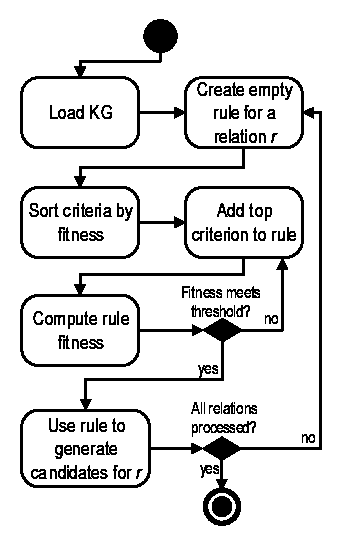
\includegraphics[width=.35\textwidth]{fig/chai/CHAI-flow}
%     \caption{Workflow of CHAI}
%     \label{fig:chai-flow}
% \end{figure}

% Class \textit{CriteriaCatalogue} contains all the available criteria that can be used to build candidate filtering rules, which can be obtained using the method \textit{getAll}. Criteria are implemented using the class \textit{Criterion}. The method \textit{apply} of this class receives a set of candidate triples, and produces a smaller, filtered set of candidates that meet the criterion in question. For example, a criterion may determine that a triple is a valid candidate if its source and target entities are less than three hops apart in the KG.

% Class \textit{FitnessFunction} is used to implement a given fitness function, which gives a numerical score to a given set of candidate triples using the \textit{evaluate} method. Some possible examples of fitness functions are the relative number of total candidate triples against the number of triples in the KG, or the percentage of candidate triples that are present in the validation split of a KG and thus more likely to be correct.

% The \textit{RuleGenerator} class is responsible for generating a candidate filtering rule for a given relation. A rule, as described in Section \ref{sec:chai-proposal}, is a conjunction of criteria that determine whether a given triple is a valid candidate or not. 

% First, a new rule is produced using the \textit{getNew} method. Then, a series of criteria are iteratively added to it in order to progressively construct it. This is done by sorting all the available criteria according to the fitness function, and then using the \textit{addCriterion} method to add the top criterion. The fitness of the resulting rule is subsequently evaluated using the \textit{evalRule} method, and this process is repeated until \textit{evalRule} returns a fitness value that meets a certain threshold.

% Finally, the \textit{Rule} instance produced by the \textit{RuleGenerator} can be used to filter candidate triples in a KG, using its \textit{apply} method. The \textit{CandidateGenerator} class handles this process, applying a given rule to the desired set of candidates and returning the set of triples that are considered promising candidates according to the rule.

\subsection{Design and performance considerations}
% The software architecture of CHAI has been devised using a number of common software patterns. First, given that only one instance of most classes is needed at runtime, all such classes have been designed as singletons, to statically guarantee a smaller memory footprint. 
% However, there are two places where a singleton cannot be used. One of them is for class Rule, since the execution of CHAI will result in the generation of one rule per relation in the KG. Another similar case is class Criterion, because it is clear that multiple different criteria should be instantiated at runtime.

% To facilitate the inclusion of new criteria in the future, they are accessed through a CriteriaCatalogue class, which takes care of detecting all available criteria in the system and loading them at runtime. This way, no further changes in the system are needed if additional criteria need to be added.

% Finally, the way in which candidates are obtained from a rule enjoys a significant optimization. Rather than following a filtering approach, where the entire set of possible candidates needs to be instantiated and then pruned, we follow a generative approach. The CandidateGenerator class is able to inspect the conditions of a rule, and then generate exclusively those candidate triples that would have been allowed by it. While the final set of filtered candidates can be proved to be the same, this results in significant runtime and memory usage improvements.

\section{Evaluation}\label{sec:chai-evaluation}
% In this section we present the experimental results that confirm that CHAI is effective in practice. First, we introduce the experimental setting. Then, we present the results of applying CHAI on several well-known Knowledge Graphs, comparing them against those of a state-of-the-art baseline technique by \citet{shi18}, which is, to the best of our knowledge, the only KG completion proposal that includes a well-defined way to filter candidate triples and experimental results on this regard. Finally, we discuss these results.

\subsection{Setup and experimental data}

% We evaluated CHAI using a number of different Knowledge Graphs that are openly available and commonly used for the task of KG completion: FB13, WN11 \cite{socher2013}, WN18 \cite{bordes2014} (which are subsets of Freebase \cite{bollacker2008} and Wordnet \cite{miller1995}, respectively), a subset of NELL introduced by \citet{gardner2015}, and EPSRC\footnote{\url{http://epsrc.rkbexplorer.com}}, which contains information about the grants provided by the Engineering and Physical Sciences Research Council of the United Kingdom. All of these Knowledge Graphs were obtained from the publicly available AYNEC-DataGen tool \cite{ayala2019}, and an overview of their metadata can be found in Table~\ref{table:chai-datasets}. We used CHAI to generate rules for every relation in every KG, except for the case of NELL, in which we focused on the same subset of 10 relations as \citet{gardner2015} due to the high number of total relations. All experiments were conducted on a computer with 32GB of RAM and an Intel Core i9-9900K CPU.

% \begin{table}[htp]
    \begin{center}
    \begin{tabular}{ M{2.5cm} | M{2.5cm} | M{2.5cm} | M{2cm} } 
    \centering \textbf{KG} & \textbf{Training triples} & \textbf{Test triples} & \textbf{Relations} \\
    \hline
    FB13 & 285,208 & 78,490 & 13 \\ 
    \hline 
    WN18 & 117,160 & 58,564 & 18 \\
    \hline 
    NELL & 201,870 & 13,491 & 519 (10) \\
    \hline 
    EPSRC & 341,372 & 85,337 & 20 \\
    \end{tabular}
    \caption{Overview of the KGs used for evaluating CHAI}
    \label{table:chai-datasets}
    \end{center}
\end{table}

% The results of the approach followed by \citet{shi18} were used as a baseline. Their proposal consists in generating candidate triples by altering the target entities of the triples already present in the KG, and replacing them by all entities that can be found in the range of the relation present in the triple. This is equivalent to applying only the $ran_{\KG, r}$ criterion, where $r$ is the relation for which CHAI is being applied. %Therefore, we obtained the baseline results by modifying CHAI to include only that criterion.

\subsection{Evaluation parameters}\label{sec:impl-details}
% To conduct our experiments, we set the distance threshold $N$ for the $distance$ criterion to 4. This value was chosen empirically, aiming to allow for a threshold as high as possible while still being reasonable in terms of computation time. Additionally, these distances were computed on a partially undirected version of the KGs. This was done to fully exploit the highly relational nature of KGs, while still not allowing paths that would be connected by means of entities with a very high in-degree such as genders or nationalities.

% The training and testing splits of the KGs were already provided by the KGs that we used, and thus we provided CHAI with these splits as is. We evaluated CHAI using a fitness function that combines reduction rate (rr) and coverage using their harmonic mean, as shown in Eq. \ref{eq:fitness-recall-rr}. The $\theta$ threshold value required by the algorithm was set to 0.99, so as to allow CHAI to find highly satisfactory rules, and to study the evolution of the coverage and reduction rate of said rules if they keep growing in size without meeting the threshold. Formally, they are defined as follows:

% \begin{equation*}
% \centering
% \begin{aligned}
% \textrm{Let}~\Sset~\textrm{be a candidates set, and}~\Sset'\subseteq \Sset~\textrm{a set of filtered candidates:}
% \end{aligned}
% \end{equation*}

% \begin{equation}
% \label{eq:fitness-recall-rr}
% \begin{gathered}
% {\ff}itness(\KG, \Sset, \Sset') = \frac{2 \cdot rr(\Sset, \Sset') \cdot coverage(\KG, \Sset')}{rr(\Sset, \Sset') + coverage(\KG, \Sset')}\textrm{\,,~where}
% \end{gathered}
% \end{equation}

% \begin{equation*}
% \label{eq:rr}
% \begin{gathered}
% rr(\Sset, \Sset') = 1 - \frac{|\Sset'|}{|\Sset|}
% \end{gathered}
% \end{equation*}

% \begin{equation*}
% \label{eq:recall}
% \begin{gathered}
% coverage(\KG = \KGlong, \Sset') = \frac{|\Sset' \cap \Tset|}{|\Tset|}
% \end{gathered}
% \end{equation*}

% This fitness function was devised under the following rationale: focusing only on coverage would result in very long rules that allow as many candidates as possible, however, this would not be desirable as we aim to reduce the size of the set of candidates, to avoid having to evaluate low-quality candidates. Conversely, focusing only on reduction rate would yield very short (and thus more restrictive) rules. As a consequence, this fitness function achieves a compromise between reduction rate and coverage, and allows for more flexibility in the lengths of the rules in contrast to focusing only on one objective. To illustrate this difference, we have also tested CHAI using two alternative fitness functions: only coverage, and only reduction rate. The results achieved by every fitness function are shown in Figure \ref{fig:chai-points-datasets}.

\subsection{Results and discussion}
% In the following, we present the results achieved by CHAI on the KGs under evaluation and the conclusions we draw from them.

% Figure \ref{fig:chai-fitness-datasets} reports on the evolution of the coverage and reduction rate for all KGs under study as rules grow in size, where each line represents a different relation; while Figure \ref{fig:chai-points-datasets} display the values for the coverage and reduction rate for every iteration in all Knowledge Graphs as points in a 2-dimensional space. Finally, Table \ref{table:recall-rr-max} provides an overview on the average maximum coverage and reduction rate that CHAI achieves for the relations in all KGs under study. This Table also includes the average coverage and reduction rate values achieved by the proposal of Shi and Weninger~\cite{shi18}, which was denoted as ``baseline'' for brevity.

% \begin{figure*}[htp]
%     \centering
%     \def\subfigscale{0.4}
%     \subfigure[FB13 - Coverage]{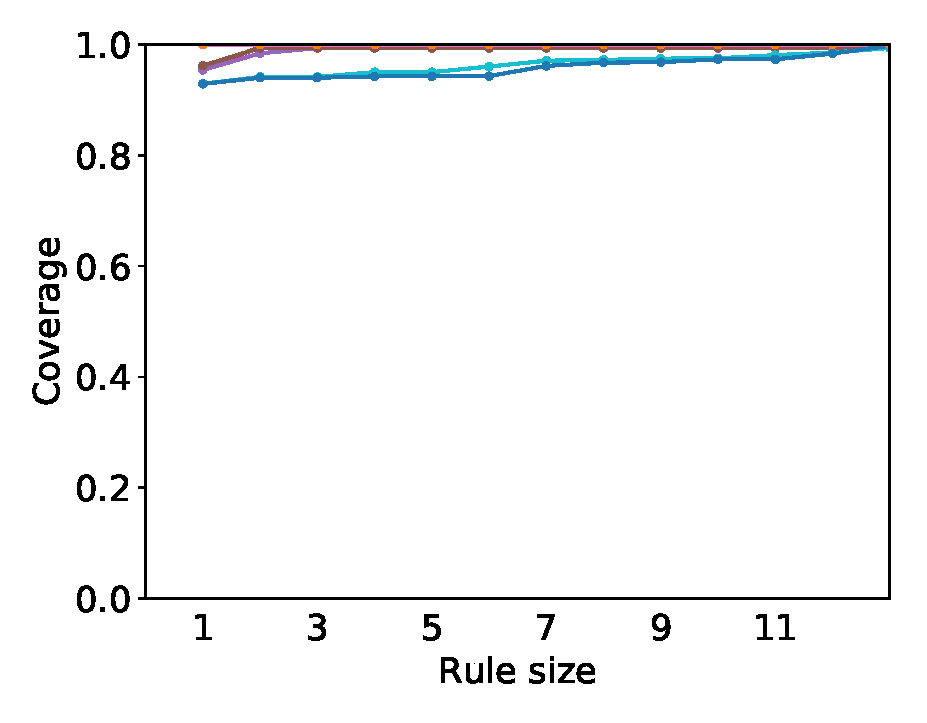
\includegraphics[scale=\subfigscale]{fig/chai/FB13_recall}\label{fig:res-FB13-recall}}~
%     \subfigure[FB13 - Reduction rate]{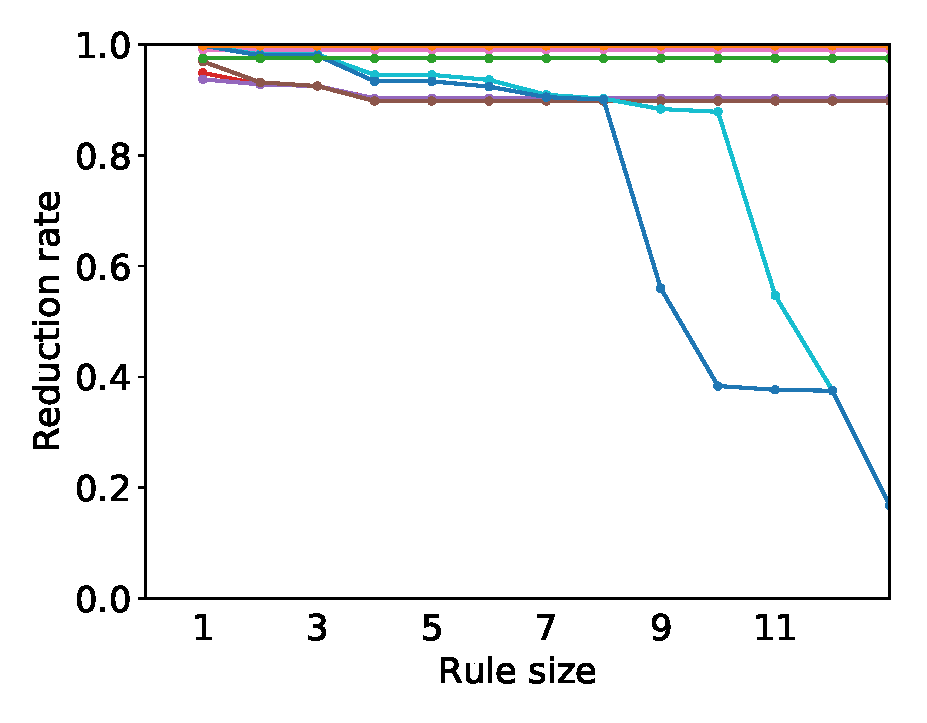
\includegraphics[scale=\subfigscale]{fig/chai/FB13_rr}\label{fig:res-FB13-rr}}\\

%     \subfigure[WN18 - Coverage]{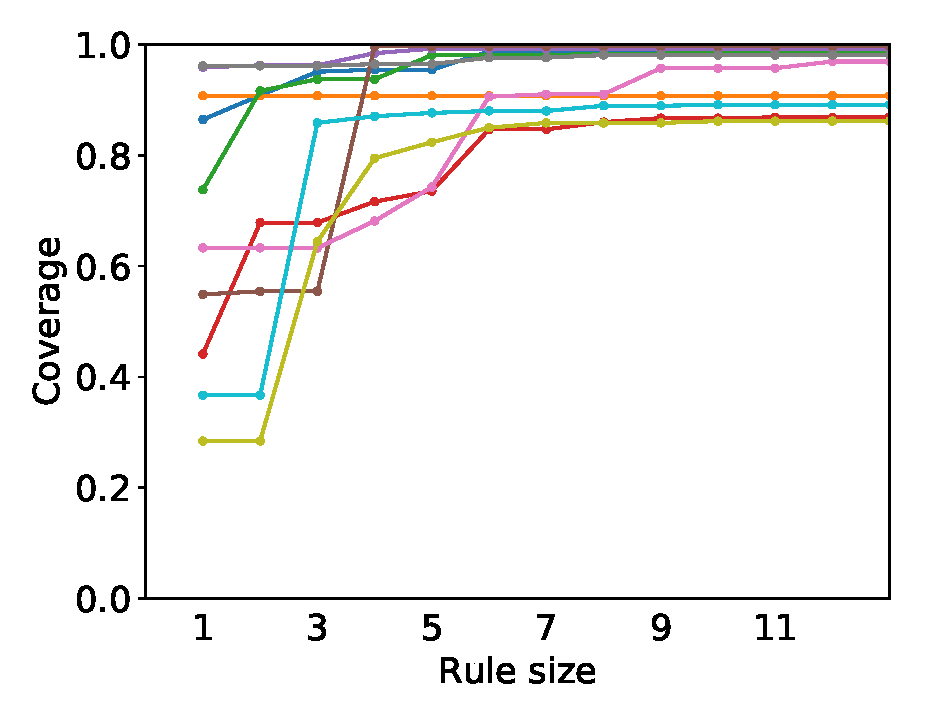
\includegraphics[scale=\subfigscale]{fig/chai/WN18-AR_recall}\label{fig:res-WN18-recall}}~
%     \subfigure[WN18 - Reduction rate]{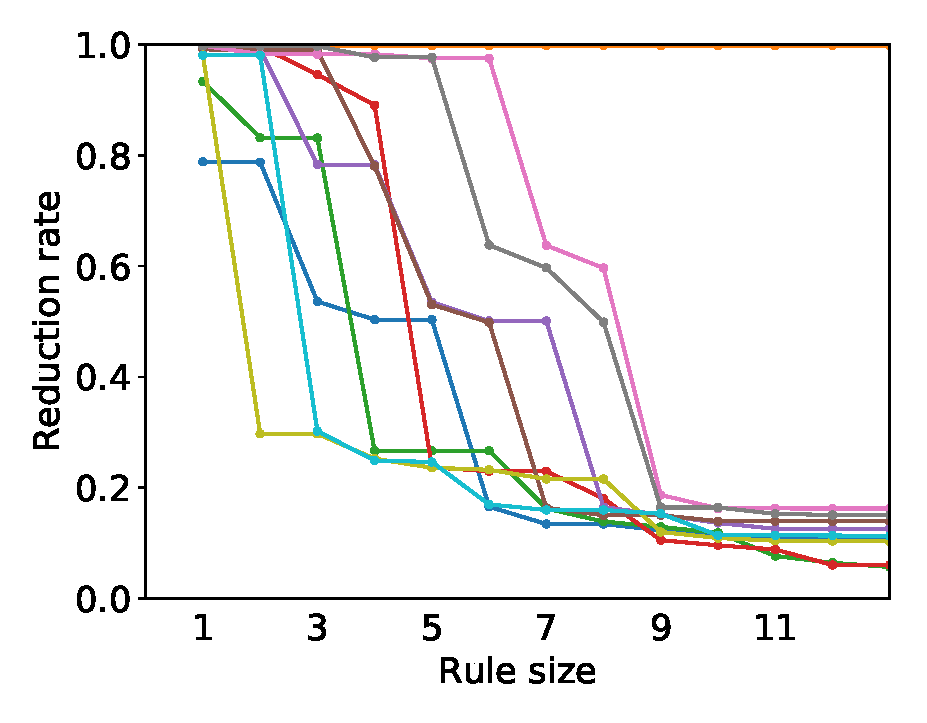
\includegraphics[scale=\subfigscale]{fig/chai/WN18-AR_rr}\label{fig:res-WN18-rr}}\\

%     \subfigure[NELL - Coverage]{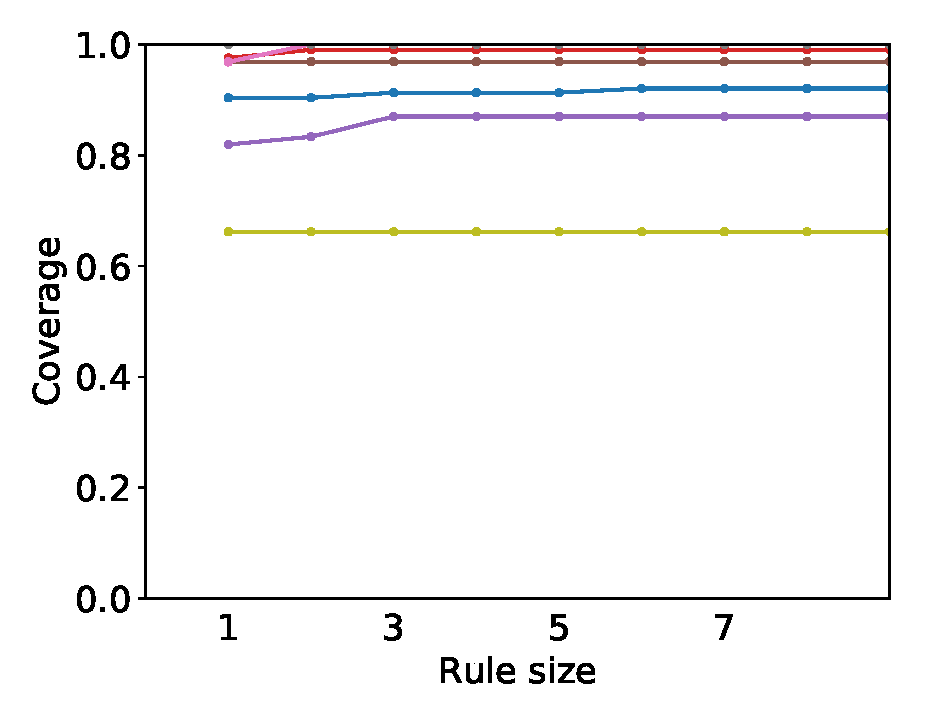
\includegraphics[scale=\subfigscale]{fig/chai/NELL-AR_recall}\label{fig:res-NELL-recall}}~
%     \subfigure[NELL - Reduction rate]{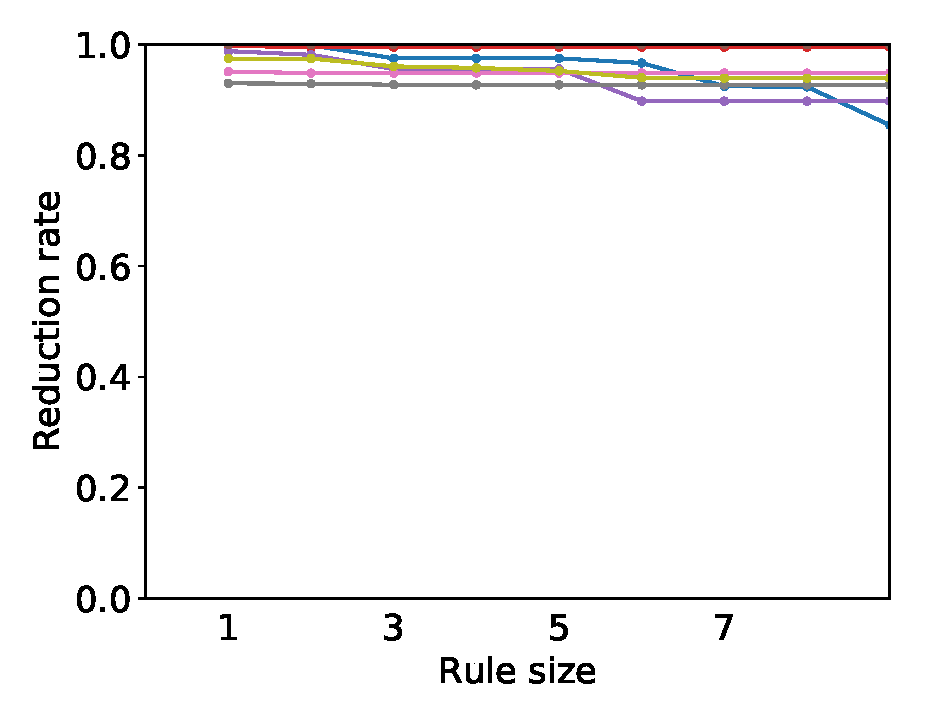
\includegraphics[scale=\subfigscale]{fig/chai/NELL-AR_rr}\label{fig:res-NELL-rr}}\\

%     \subfigure[EPSRC - Coverage]{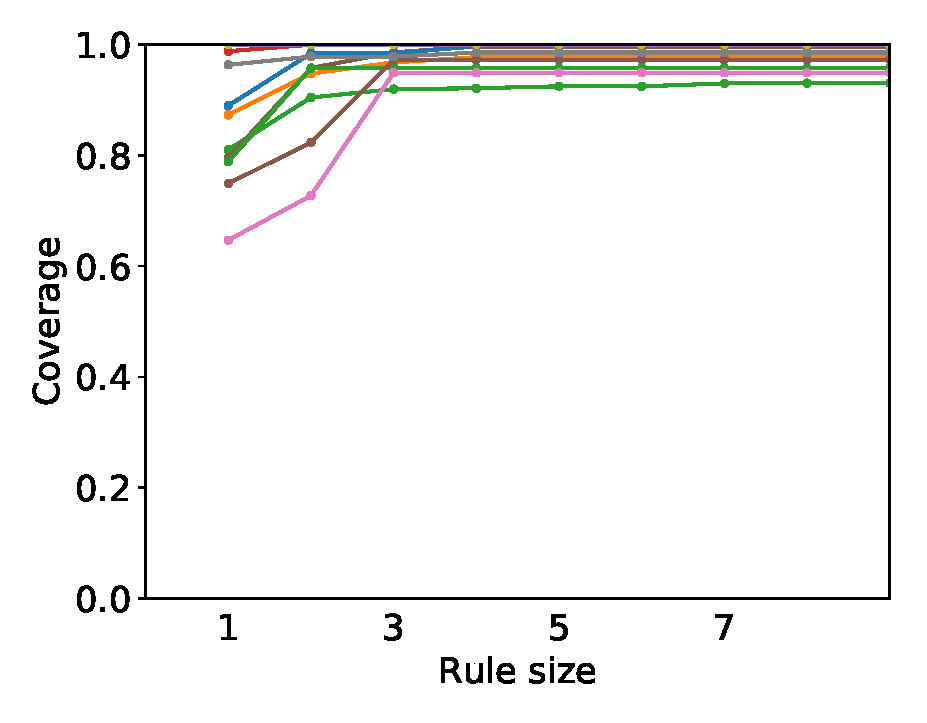
\includegraphics[scale=\subfigscale]{fig/chai/epsrc_recall}\label{fig:res-EPSRC-recall}}~
%     \subfigure[EPSRC - Reduction rate]{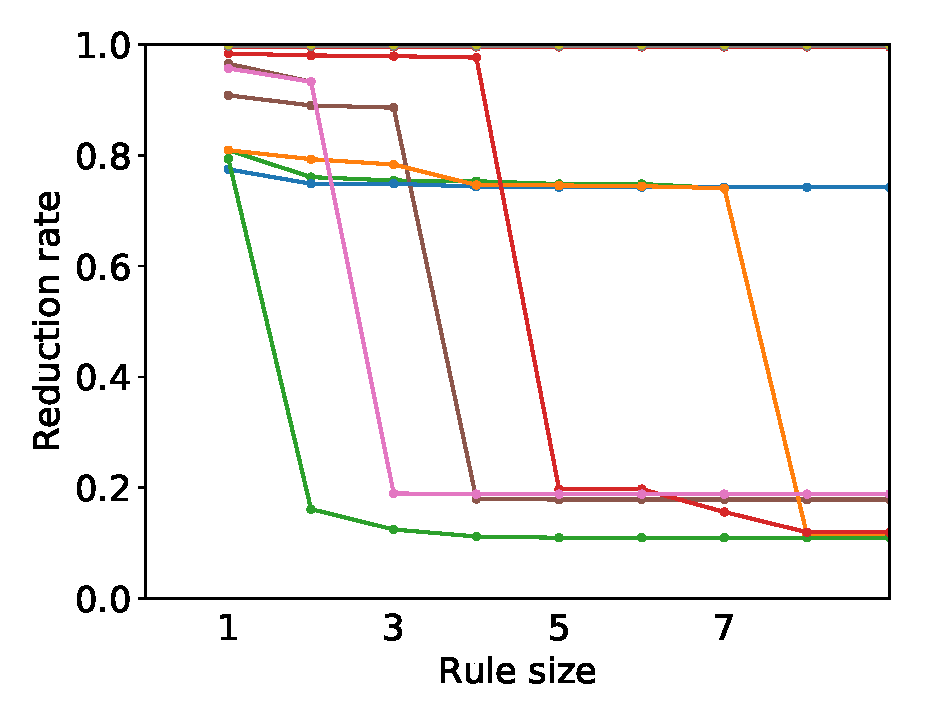
\includegraphics[scale=\subfigscale]{fig/chai/epsrc_rr}\label{fig:res-EPSRC-rr}}\\

%     \caption{Evolution of the coverage (left) and reduction rate (right) values}
%     \label{fig:chai-fitness-datasets}
% \end{figure*}

% \begin{figure}[htp]
%     \centering
%     \def\subfigscale{0.4}
%     \subfigure[FB13]{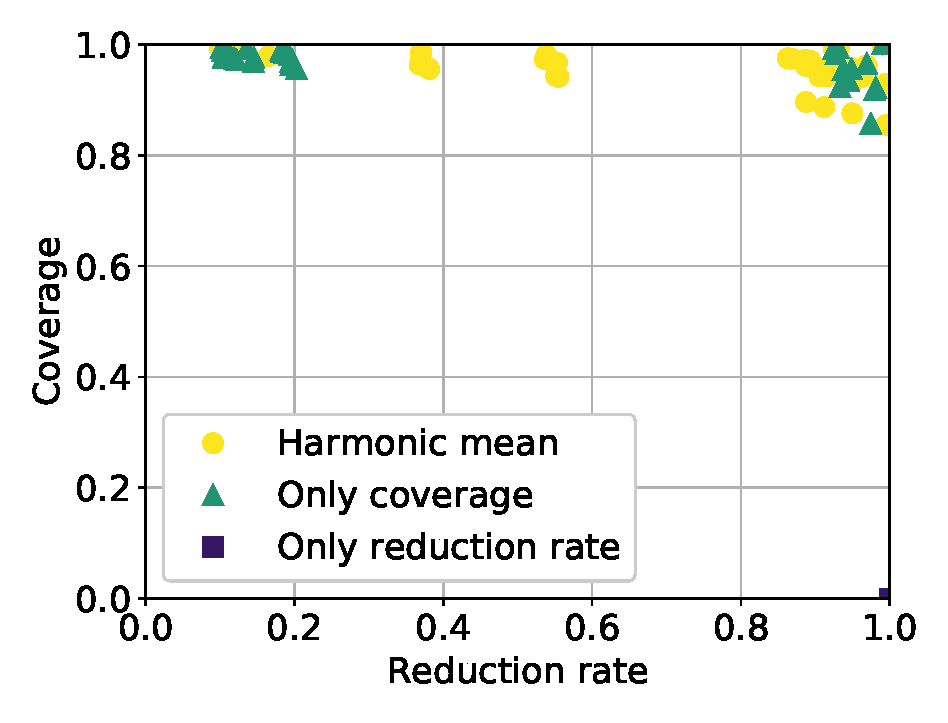
\includegraphics[scale=\subfigscale]{fig/chai/FB13_points}\label{fig:res-FB13-points}}~
%     \subfigure[WN18]{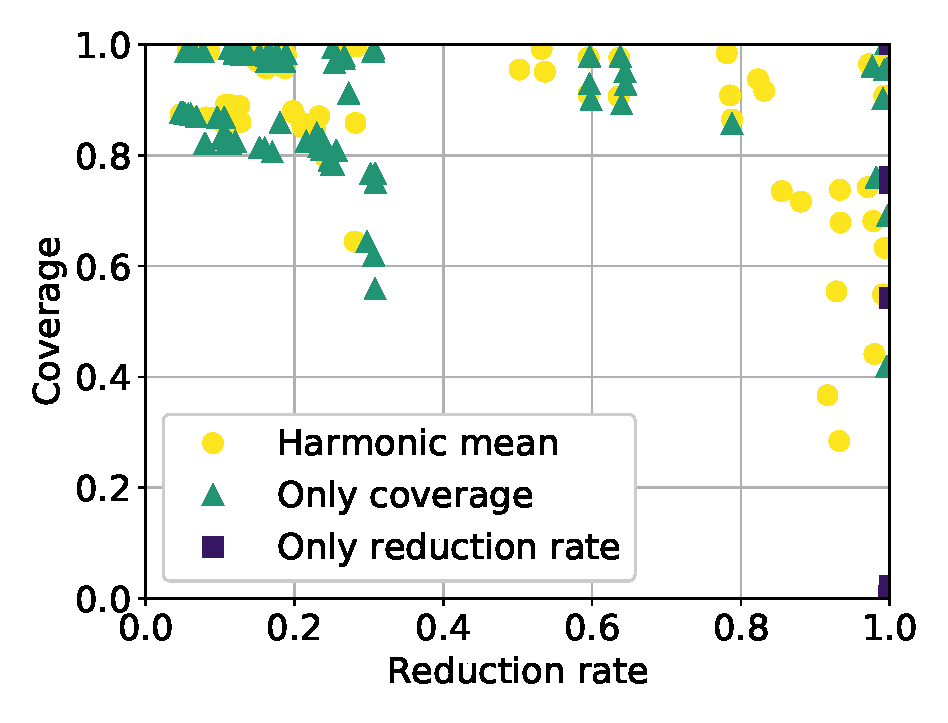
\includegraphics[scale=\subfigscale]{fig/chai/WN18-AR_points}\label{fig:res-WN18-points}}
%     \subfigure[NELL]{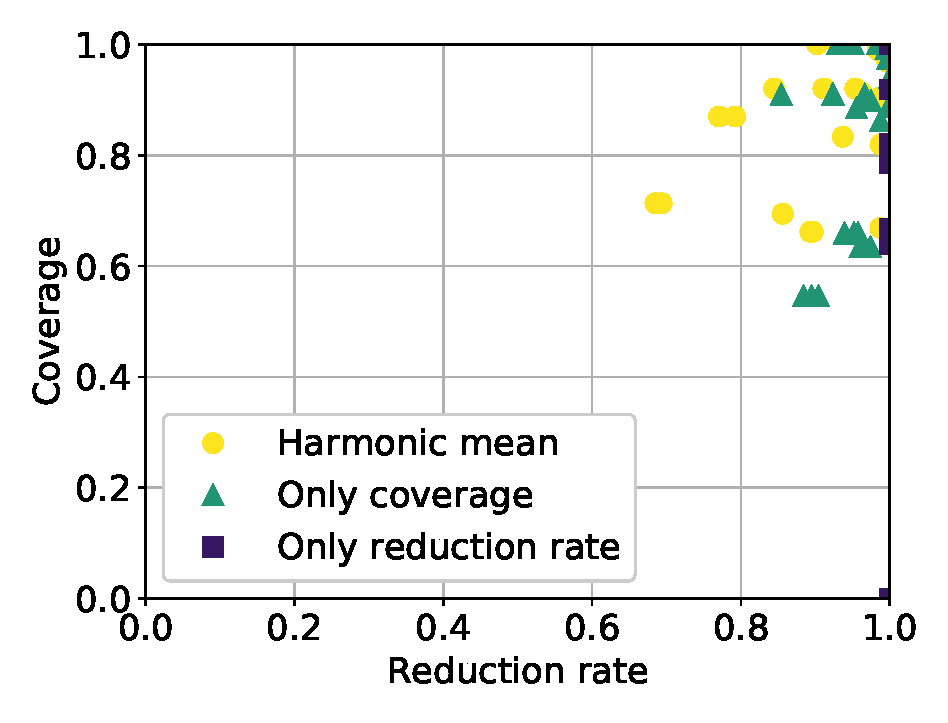
\includegraphics[scale=\subfigscale]{fig/chai/NELL-AR_points}\label{fig:res-NELL-points}}~
%     \subfigure[EPSRC]{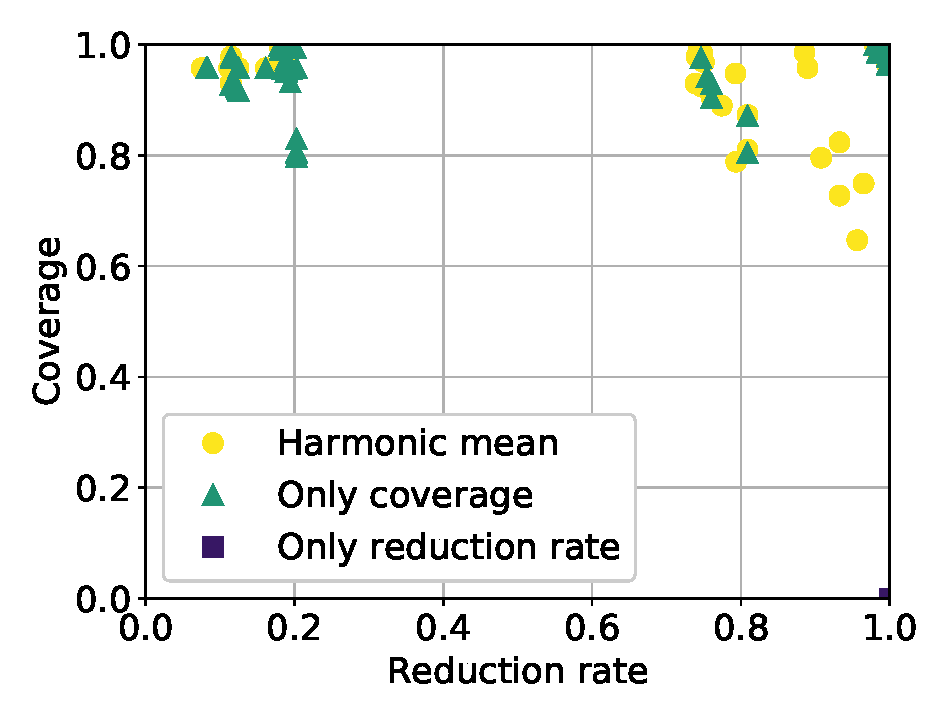
\includegraphics[scale=\subfigscale]{fig/chai/epsrc_points}\label{fig:res-EPSRC-points}}
%     \caption{Reduction rate (x) and coverage (y) for different fitness functions}
%     \label{fig:chai-points-datasets}
% \end{figure}

% \begin{table}[htp]
    \begin{center}
    \begin{tabular}{ M{1.5cm} | M{2.5cm} | M{2.5cm} | M{2.5cm} | M{2.5cm} } 
    \centering \textbf{KG} & \textbf{Avg. max. coverage (CHAI)} & \textbf{Avg. coverage (baseline)} & \textbf{Avg. max. RR (CHAI)} & \textbf{Avg. RR (baseline)} \\
    \hline
    FB13 & \textbf{0.92} (0.76-1.00) & \textbf{0.78} (0.58-0.99) & \textbf{0.91} (0.76-1.00) & \textbf{0.91} (0.76-1.00) \\ 
    \hline 
    WN18 & \textbf{0.94} (0.89-0.99) & \textbf{0.49} (0.26-0.72) & \textbf{0.97} (0.93-1.00) & \textbf{0.93} (0.85-1.00) \\
    \hline 
    NELL & \textbf{0.89} (0.78-1.00) & \textbf{0.53} (0.26-0.80) & \textbf{0.97} (0.95-1.00) & \textbf{0.99} (0.99-1.00) \\
    \hline 
    EPSRC & \textbf{0.99} (0.98-1.00) & \textbf{0.82} (0.68-0.97) & \textbf{0.95} (0.91-0.99) & \textbf{0.95} (0.92-0.99) \\
    \end{tabular}
    \end{center}
    \caption{Max. coverage and reduction rate values (avg and 95\% conf.)}
    \label{table:recall-rr-max}
\end{table}

% These results allow us to distinguish between two types of relations: those for which a high coverage value is obtained with a very short rule, and those for which the coverage starts at a lower value and increments as rules grow in size, as shown in Figure \ref{fig:chai-fitness-datasets}. We consider the former type of relations to be categorical, as they have a range of possible target entities that is relatively small: for example, the entities that are targets for the relation \textit{location} are unlikely to appear as the target for any other relation, and thus using the entities that are targets for \textit{location} as possible candidates for locations yields a very good result. On the other hand, relations that are non-categorical have a much wider range of possible candidates: in the case of the relation \textit{children}, an entity may produce a good candidate even if it does not appear as the target of \textit{children} (for example, they may appear in the relation \textit{sibling}).

% This conclusion is reinforced by the results shown in Figure \ref{fig:chai-points-datasets}, where there are groups of iterations in the top-right corner (the area of both high reduction rate and high coverage), which are obtained for categorical relations with a small subset of possible targets, while a different group of iterations show more scattered results in the top area, denoting that in order to achieve a high coverage, a bigger set of candidates must be used (non-categorical relations). Additionally, the results shown in this Figure lead us to the conclusion that using only reduction rate as the fitness function results in a very poor coverage, as the algorithm stops after having selected only one criterion that allows a very small number of candidates. On the contrary, using only coverage as the fitness function provides better results, but with a clear tendency towards prioritizing coverage at the expense of a lower reduction rate, while using the harmonic mean yields more balanced results.

% In the case of non-categorical relations, there exists a trade-off between coverage and reduction rate. This is to be expected, since rules are disjunctions of criteria and thus rules that comprise more criteria are more likely to filter out less candidates, increasing coverage but decreasing the reduction rate. In these cases, it is up to the user to decide whether they are interested in achieving a very high coverage with a lower reduction rate, or a higher reduction rate with a usually lower coverage. For this kind of relations, distance-based criteria are generally useful: for example, one's parents or spouse are usually found within a short distance in the KG. In categorical relations, however, one is able to obtain both a high reduction rate and a high coverage, because the entities that are suitable targets for said relations can easily be found by analyzing the domains and ranges of the relation in question or other relations.

% Regarding the reduction rate, it must be noted that it is computed with regard to the set of candidates that are selected by the $exists$ criterion, and not with respect to the Cartesian product of all possible candidates. This results in reduction rates that are in all cases lower than those that would be obtained in the latter case, though more evenly spread between 0 and 1. Given that high reduction rates are still achieved, we do not consider this to be a problem, but rather an adequate way of measuring how many candidates are selected with respect to an initial set of filtered candidates, with many unlikely candidates already filtered out.

% Finally, it is worth noting that CHAI consistently manages to achieve high coverage values for all Knowledge Graphs under study, as it can be seen in Figure \ref{fig:chai-fitness-datasets}. These values start to converge with rules composed of approximately five criteria, and thus we find that the criteria that are ranked higher by means of the proposed fitness function (Eq. \ref{eq:fitness-recall-rr}) are indeed successful in allowing promising candidates to pass the filter. When comparing CHAI to the baseline approach proposed by \citet{shi18}, CHAI achieves much higher values of coverage while still being able to obtain similar reduction rates, as shown in Table \ref{table:recall-rr-max}. The values for CHAI shown in said Table refer to the average maximum values that can be achieved, and thus our proposal is more versatile as it allows the user to prioritize a higher coverage by using longer rules, or a higher reduction rate by using shorter rules. CHAI works well for all kinds of relations due to the versatility of the criteria it uses, while the proposal by \citet{shi18} is not able to deal as effectively with non-categorical relations in terms of coverage, hindering its overall performance.


\section{Limitations}\label{sec:chai-limitations}
% While CHAI obtains satisfactory results, it is not without limitations. Perhaps the most important one would arise in the case of a KG with a very high number of total relations, because the amount of domain and range-based criteria would be equally high. In this case, the fitness function would have to be computed for every criterion in order to sort them by decreasing fitness value, resulting in a potentially high computational cost. Besides, CHAI may not work as well in very sparse KGs where all or most relations share the same entities in their domains and ranges, because the distance-based criterion would need a much higher threshold due to the sparsity of possible paths, and the domain and range-based ones would not prove useful.

\section{Summary}\label{sec:chai-summary}
In this chapter we have introduced CHAI, our proposal to filter candidate triples for Knowledge Graph completion. CHAI works by producing candidate filtering rules by combining a set of criteria in such a way that it optimizes a fitness function. Furthermore, CHAI produces a rule for every distinct relation in the KG, thus ensuring that the result of applying such rules is specifically tailored to the nature of every relation. Our experimental evaluation shows that CHAI is effective in practice, producing sets of candidate triples that are considerably smaller than other state-of-the-art approaches to this task, while still containing most of the candidates that could be considered promising.
    \chapter{CAFE: Our triple classification proposal}\label{chap:cafe}

\chapterQuote{\hfill\textit{``Coffee, the finest organic suspension ever devised.''}}{--- Star Trek: Voyager}

\chapterAbstract{W}{hen a set of candidate triples has been obtained, the next step in Knowledge Graph completion is to classify every triple in said set to determine if it represents correct knowledge or not and, if found to be correct, added back to the KG in order to enrich it. In this chapter we introduce CAFE, our proposal for candidate triple classification. This chapter is structured as follows: Section~\ref{sec:cafe-intro} introduces it, Section~\ref{sec:cafe-proposal} presents the neighborhood-aware features that CAFE uses to discern between correct and incorrect triples, as well as the process it follows to do so, Section~\ref{sec:cafe-architecture} discusses its internal architecture and the design choices behind it, Section~\ref{sec:cafe-evaluation} shows the experiments that we carried out to assess the effectivity of CAFE, as well as their results; Section~\ref{sec:cafe-limitations} discusses its practical limitations; finally, Section~\ref{sec:cafe-summary} summarizes the chapter.}

\section{Introduction}\label{sec:cafe-intro}
This chapter presents CAFE~\cite{borrego2021}, our proposal for triple classification. CAFE covers the second main step in Knowledge Graph completion: once an adequately small set of candidate triples has been obtained, every triple in it must be carefully evaluated to determine whether or not it represents correct knowledge and, if so, added to the KG to enrich and expand it.

CAFE works by transforming any possible triple into a numerical vector by using a novel set of neighborhood-aware features, which measure the correctness of a triple leveraging its context in a Knowledge Graph. By transforming all triples into vectors in this manner, CAFE trains and uses a binary classifier to discern between correct and incorrect triples.

We thoroughly evaluate CAFE using several well-known Knowledge Graphs, and our evaluation shows that it is able to achieve a high precision in challenging, real-world scenarios, thus allowing for a trustworthy KG completion process.

Over the course of this chapter, we continue to follow the running example introduced in Section~\ref{sec:theo-intro}.


\section{Our proposal}\label{sec:cafe-proposal}
As previously described, the second major step when completing a Knowledge Graph consists of analyzing the set of possible candidate triples, assessing which ones represent correct knowledge, and adding them back to the KG in order to augment it. In this step, it is important to achieve a high precision, in order to have a Knowledge Graph completion process that is as trustworthy as possible~\cite{shen2022overview}.

To carry out this process, we have devised CAFE, a technique that classifies candidate triples into correct or incorrect ones. Given a Knowledge Graph and a set of candidate triples, CAFE evaluates each one of them and assigns them a binary label, denoting whether it should be considered correct and added to the Knowledge Graph, or incorrect and discarded. CAFE does this by defining a set of neighborhood-aware features, which checks for shared neighborhoods at several distance levels and under certain conditions, under the assumption that the entities in correct triples usually have a higher degree of overlap in their neighborhoods. Then, using these features, each candidate triple is converted into a numerical vector. Finally, CAFE trains a number of neural classification models using these vectors to learn to separate correct triples from incorrect ones. In the following subsections, we describe the features and architecture of CAFE in detail.

\subsection{Neighborhood-aware features}\label{sec:cafe-features}
We propose a set of neighborhood-aware features that takes neighborhood subgraphs, reachable entities and paths into account. Due to the large number of possible variations of each feature, we present our feature set in terms of groups of features. Each group can be parameterized to obtain a specific feature, which we call an instance of the feature group.

For the sake of example, we illustrate a possible instance of every feature group and its value using the example triple $example = $\tripleSty{(Daniel Radcliffe, plays, Harry Potter)}, and the KG shown in Figure~\ref{fig:kg-potter}.

\featgroup{Number of entities in the neighborhood subgraph of size \texorpdfstring{$n$}{n} of the source entity in the triple.}
{n}
{|\Eset{}_s^n|}
{fig:kg-potter}
{2}
{$|\{$\textit{Daniel Radcliffe, Harry Potter and the Goblet of Fire (movie), Harry Potter and the Prisoner of Azkaban (movie), Harry Potter and the Goblet of Fire (book), Harry Potter and the Prisoner of Azkaban (book)}$\}| = 5$}


\featgroup{Number of entities in the neighborhood subgraph of size \texorpdfstring{$n$}{n} of the target entity in the triple.}
{n}
{|\Eset{}_t^n|}
{fig:context-examples-b}
{3}
{$|\{$\textit{Harry Potter, J.K. Rowling, Harry Potter and the Goblet of Fire (book), Harry Potter and the Prisoner of Azkaban (book), Robin Ellacott, Hermione Granger}$\}| = 6$}

\featgroup{Degree of N-path centrality of the source entity in the triple.}
{n}
{\frac{|\Eset{}_s^n|}{|\Eset| - 1}}
{fig:context-examples-a}
{1}
{$|\{$\textit{Harry Potter and the Goblet of Fire (movie), Harry Potter and the Prisoner of Azkaban (movie)}$\}| / (13 - 1) = 2 / 12 \approx 0.17$}

\featgroup{Degree of N-path centrality of the target entity in the triple.}
{n}
{\frac{|\Eset{}_t^n|}{|\Eset| - 1}}
{fig:context-examples-b}
{1}
{$|\{$\textit{Harry Potter and the Goblet of Fire (book), Harry Potter and the Prisoner of Azkaban (book)}$\}| / (13 - 1) = 2 / 12 \approx 0.17$}

\featgroup{Number of common entities between the neighborhood subgraph of size \texorpdfstring{$n$}{n} of the source entity and the neighborhood subgraph of size \texorpdfstring{$m$}{m} of the target entity in the triple.}
{n, m}
{|\Eset{}_s^n \cap \Eset{}_t^m|}
{fig:context-examples}
{2, 3}
{$|\{$\textit{Harry Potter and the Goblet of Fire (book)}, \textit{Harry Potter and the Prisoner of Azkaban (book)}$\}| = 2$}

\featgroup{Jaccard index of similarity between the entities in the neighborhood subgraph of size \texorpdfstring{$n$}{n} of the source entity and the neighborhood subgraph of size \texorpdfstring{$m$}{m} of the target entity in the triple.}
{n, m}
{jaccard(\Eset{}_s^n, \Eset{}_t^m)}
{fig:context-examples}
{2, 3}
{$|\{$\textit{Harry Potter and the Goblet of Fire (book), Harry Potter and the Prisoner of Azkaban (book)}$\}|$~$/$~$|\{$\textit{Daniel Radcliffe, Harry Potter and the Goblet of Fire (movie), Harry Potter and the Prisoner of Azkaban (movie), Harry Potter and the Goblet of Fire (book), Harry Potter and the Prisoner of Azkaban (book), Harry Potter, J.K. Rowling, Robin Ellacott, Hermione Granger}$\}| = 2~/~9 = 0.22$}

\featgroup{Adamic-Adar index of closeness between the neighborhood subgraphs of size \texorpdfstring{$n$}{n} of the source and target entities in the triple.}
{n}
{\sum_{e \in \nearby{s}{n} \cap \nearby{t}{n}}{\frac{1}{log |\nearby{e}{n}|}}}
{fig:context-examples}
{2}
{$\frac{1}{log |\nearby{\textit{\footnotesize Harry Potter and the Goblet of Fire (book)}}{2}|} = \frac{1}{log |3|} \approx 2.09$}

\featgroup{Number of reachable entities through the relation \texorpdfstring{$r$}{r} at distance \texorpdfstring{$n$}{n} from the source entity in the triple.}
{r, n}
{|Reachable(s, r, n)|}
{fig:context-examples-a}
{\textit{hasPrequel}, 2}
{$|\{$\textit{Daniel Radcliffe, Harry Potter and the Prisoner of Azkaban (movie)}$\}| = 2$}

\featgroup{Number of reachable entities through the relation \texorpdfstring{$r$}{r} at distance \texorpdfstring{$n$}{n} from the target entity in the triple.}
{r, n}
{|Reachable(t, r, n)|}
{fig:context-examples-b}
{\textit{created}, 2}
{$|\{$\textit{Harry Potter,Hermione Granger, Robin Ellacott}$\}| = 3$}

\featgroup{Number of common reachable entities through the relation \texorpdfstring{$r$}{r} from the source entity at distance \texorpdfstring{$n$}{n} and from the target entity at distance \texorpdfstring{$m$}{m}.}
{r, n, m}
{\\|Reachable(s, r, n) \cap Reachable(t, r, m)|}
{fig:context-examples}
{\textit{created}, 2, 3}
{$|\{$\textit{Daniel Radcliffe}$\} \cap \{$\textit{Harry Potter, Hermione Granger, Robin Ellacott}$\}| = 0$}

\featgroup{Jaccard index of similarity between the reachable entities through the relation \texorpdfstring{$r$}{r} from the source entity at distance \texorpdfstring{$n$}{n}, and those reachable through the relation \texorpdfstring{$r$}{r} from the target entity at distance \texorpdfstring{$m$}{m}.}
{r, n, m}
{\\jaccard(Reachable(s, r, n), Reachable(t, r, m))}
{fig:context-examples}
{\textit{created}, 2, 3}
{$|\emptyset|$~$/$~$|\{$\textit{Harry Potter, Hermione Granger, Robin Ellacott}$\}| = 0~/~3 = 0$}


\featgroup{Number of distinct paths of length \texorpdfstring{$n$}~ between the source and the target entity in the triple, using  relations \texorpdfstring{$r_1, \ldots, r_n$}{r1, ..., rn}.}
{n, r\textsubscript{1}, \ldots, r\textsubscript{n}}
{|\kgpathP{s}{t}{r_1,\ldots, r_n}|}
{fig:kg-example}
{4, \textit{starred\_in, based\_on, writer, created}}
{$1$, as there is one path of length 4 between the entities \textit{Daniel Radcliffe} and \textit{Harry Potter} that matches the given relations}

% Discussion of features
The rationale behind this set of features is manifold. Regarding $f_1$ and $f_2$, knowing the size of the neighborhood of an entity can be helpful to determine whether said neighborhood encompasses relevant information. For instance, our hypothesis is that very large neighborhoods tend to contain a higher amount of unrelated information. The same idea is leveraged in $f_3$ and $f_4$, which provide normalized indices of centrality with respect to the total amount of entities in the KG. Following the previous reasoning, we hypothesize that entities with large indices of centrality (i.e. highly connected to other entities) will yield less useful information. Meanwhile, feature groups $f_5$, $f_6$ and $f_7$ measure the degree of overlap that exists in the neighborhoods of the two entities, both in absolute and in relative terms, under the assumption that correct triples have a higher degree of overlap between the neighborhoods of their entities.

The previously discussed feature groups do not consider the specific relations involved. However, we deem it reasonable to assume that some relations may be more useful than others to determine whether a triple is correct, depending on their specific semantics. For example, having one or more children in common can be an indication of a marriage, while having the same nationality is not. In order to exploit this fine-grained information, feature groups $f_8$, $f_9$, $f_{10}$ and $f_{11}$ are similar to the previously discussed groups but restrict themselves to only one relation. These groups are computed for every relation in a KG.

Finally, feature group $f_{12}$ allows CAFE to find the number of paths that exist between two entities for any given relations. It is our intuition that correct triples have more alternative paths between the two entities they contain than false ones.

\subsection{Workflow}
Our proposal, CAFE, receives a KG and a set of relations from that KG as input, and outputs a classification model for each of the provided relations. These models are able to determine if a given triple that represents an instance of the relation is correct and should belong to the KG. Its workflow is depicted in Figure~\ref{fig:workflow-cafe} and, in the following, we describe each of its steps.

\begin{figure}[htp]
    \centering
    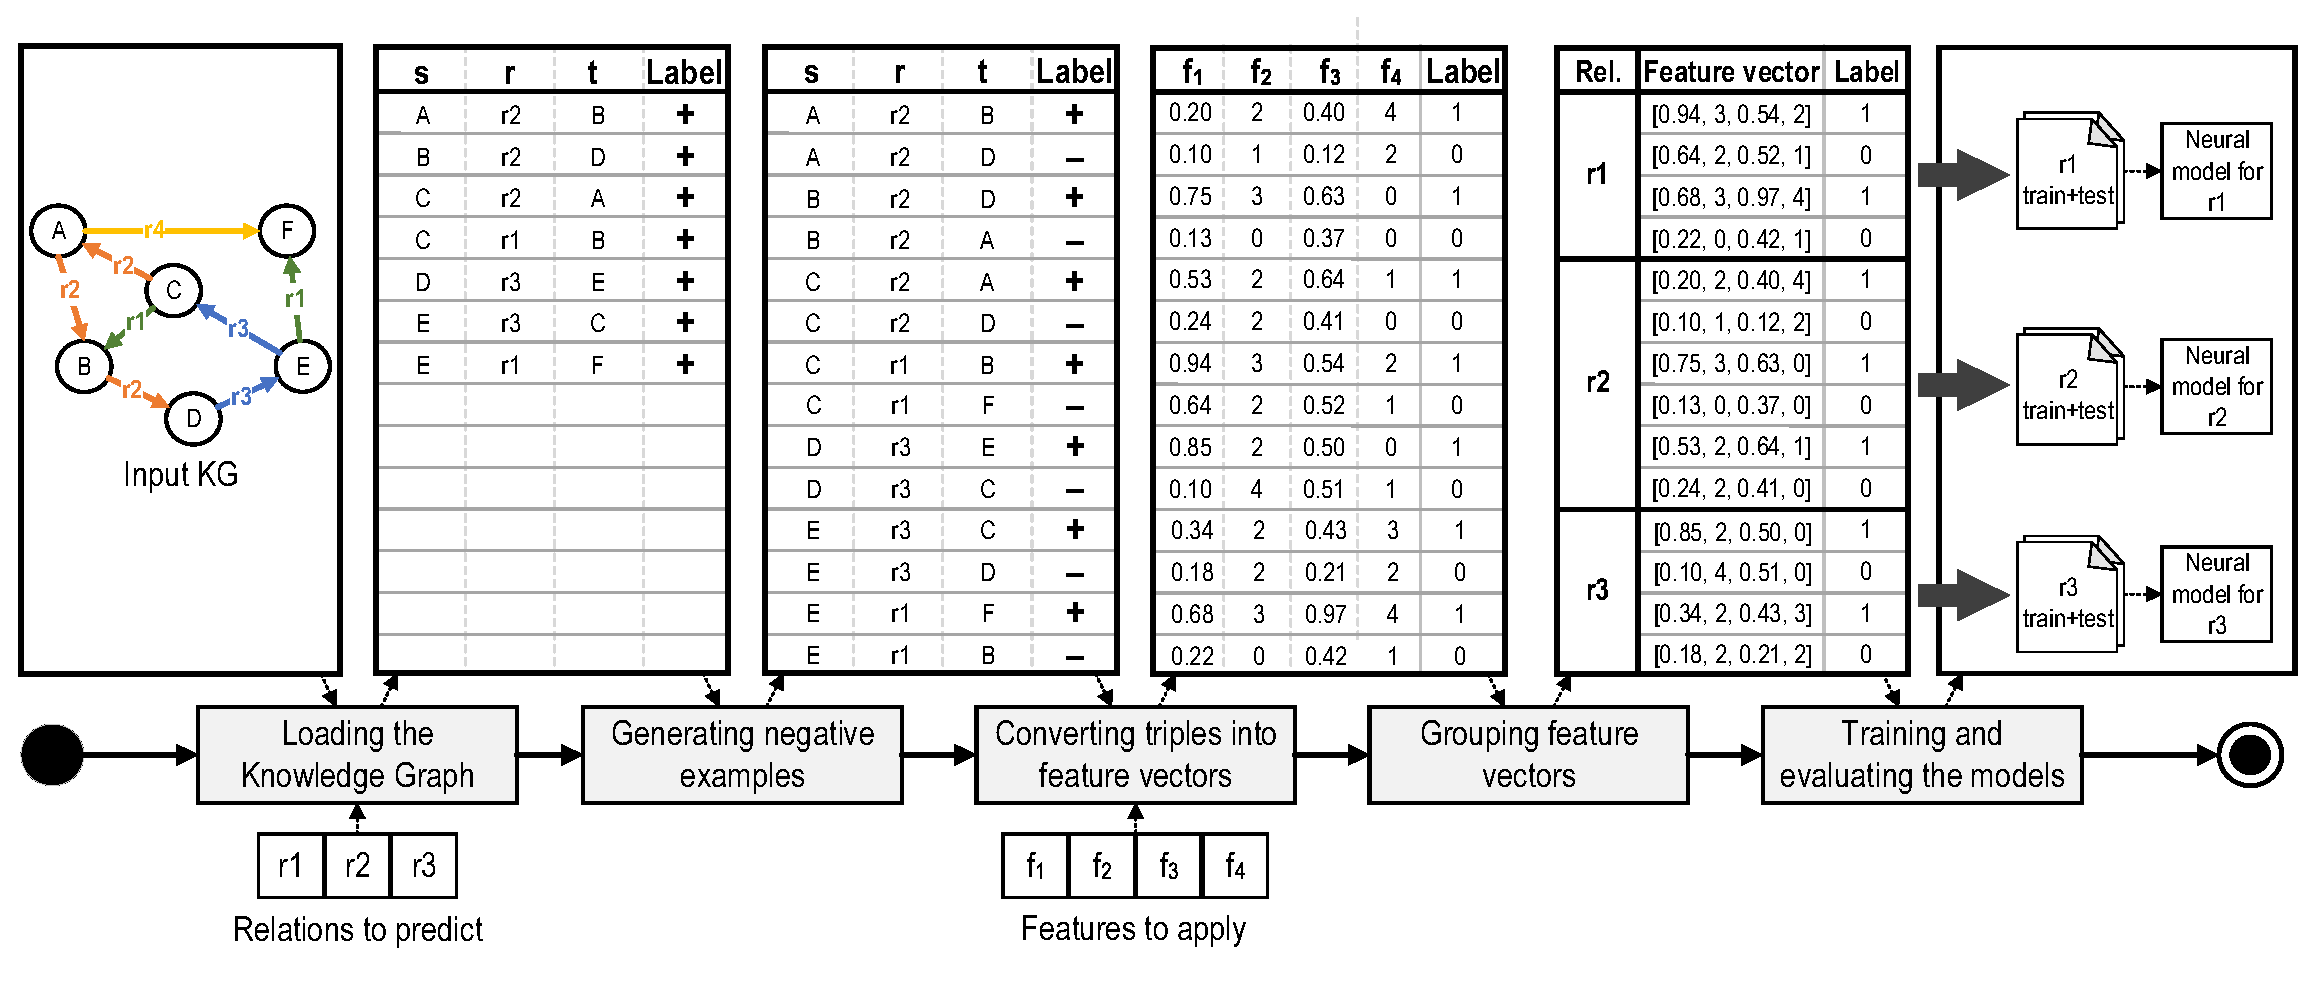
\includegraphics[width=\textwidth]{fig/cafe/workflow}
    \caption{In-depth view of the CAFE workflow}
    \label{fig:workflow-cafe}
\end{figure}

\begin{itemize}
    \item \textbf{Loading the Knowledge Graph:} CAFE internally stores the input KG in the form of \triple{} triples, using an efficient data structure based on hash tables, which is suitable for a high frequency of read operations due to its O(1) lookup times. The triples that contain relations for which a predictive model does not need to be generated are still taken into account when computing features, since they may provide valuable predictive information, but they are not transformed into feature vectors in the following steps.\\
    
    \item \textbf{Generating negative examples:} A Knowledge Graph contains only positive information, i.e., it contains examples of the occurrence of a relation $r$ between two entities. However, it does not contain explicit information about pairs of entities for which $r$ does not hold. Our proposal relies on a classification model that requires negative examples for training, which means that a number of negatives for each positive triple must be produced. To accomplish this, we follow the type-constrained local closed world assumption \cite{bansal2020negatives}, i.e., we generate negative examples from every triple \triple{} present in a KG by replacing their target entity $t$ with a different one, $t'$, such that the resulting triple \negtriple{} does not exist in the KG. Furthermore, to preserve the range of each relation, we randomly choose $t'$ such that there exists some other triple in the KG where $t'$ appears as the target entity for the relation $r$. This is known as type constraint.\\

    In the example depicted in Figure \ref{fig:kg-potter}, a valid negative example is \tripleSty{(Hermione Granger, appears\_in, The Cuckoo's Calling)}, since we know that \tripleSty{The Cuckoo's Calling} is a valid target for the relation \tripleSty{appears\_in}. However, \tripleSty{(Hermione Granger, appears\_in, Daniel Radcliffe)} would not be allowed as a negative example, because \tripleSty{Daniel Radcliffe} never appears as the target of the relation $appears\_in$.\\
    
    It can be argued that generating negative evidence in this manner can produce false negatives by mere chance, i.e., statements that are deemed incorrect but that are true in the real world. While this is indeed plausible, it is generally accepted~\cite{ji2015, lin2015, socher2013} that the chances of this happening are very low and, as a consequence, the possible effects on the final results are not significant.\\

    \item \textbf{Converting triples into feature vectors:} Once negative examples have been generated, our feature set is instantiated and applied to all triples. For all feature groups, we obtain all possible feature instances by applying all possible combinations of the values of their parameters. Each feature instance assigns a real number to each triple. Therefore, applying several features to a triple results in a feature vector. Each position of the feature vector represents that real number that the corresponding feature assigned to the triple.\\

    It is important to note that, to compute features on a positive training triple, we temporarily remove it from the KG, since not doing so would result in trivial prediction models such as ``a person plays a character if there exists a triple in the KG stating that the person plays that character''.\\\newpage

    \item \textbf{Grouping feature vectors:} The previous step computes feature vectors of triples. Since these triples can be either positive or negative, the feature vectors are accordingly labeled as positive or negative. Based on the labeled feature vectors, we train a classification model for each relation that predicts whether a triple should be added to the KG. We do this in order to allow the models to capture meaningful and distinctive information for every relation: even though the same set of features is applied to all triples, some features might have more predictive power for a relation, and other features may be more helpful for a different one.\\
    
    \item \textbf{Training and evaluating the models:} For every relation that we predict, we create one or more neural models, where each model focuses only on the features that are obtained from a certain neighborhood size. Thus, using only neighborhood subgraphs of size 1 results in one model, using neighborhood subgraphs of size of up to 2 results in two models, and so on. This allows each model to capture the specific information that every neighborhood size may yield. To combine two or more models, we use an additional combination layer to produce a single output.

    The neural models are trained using the labeled feature vectors in the training split for the desired relation, where each model receives only the features corresponding to its assigned neighborhood size, and the label or ground truth is shared among them. Prior to training our models, we first remove any individual features that have the exact same value in every feature vector and thus lack any predictive power. An example of this are path-based features ($f_{12}$), since only a small subset of all possible paths of fixed length occur between two given entities, and as a consequence most of them have a value of 0.
    
    It is important to note that we use neural classification models because they have been shown to consistently achieve satisfactory results in many different classification tasks~\cite{aggarwal2012, yadav2019, ayala2020}, although other classification models that make use of our features could be used in this step.
\end{itemize}

\section{Software Architecture}\label{sec:cafe-architecture}
We show the internal class architecture of CAFE in Figure~\ref{fig:cafe-diagram}, and its data workflow is displayed in Figure~\ref{fig:cafe-flow}. We further describe and discuss the architecture of CAFE in the following.

\begin{figure}[!htp]
    \centering
    \includesvg[width=1.0\textwidth]{fig/cafe/CAFE-classes}
    \caption{Architecture of CAFE}
    \label{fig:cafe-diagram}
\end{figure}

\begin{figure}[!htp]
    \centering
    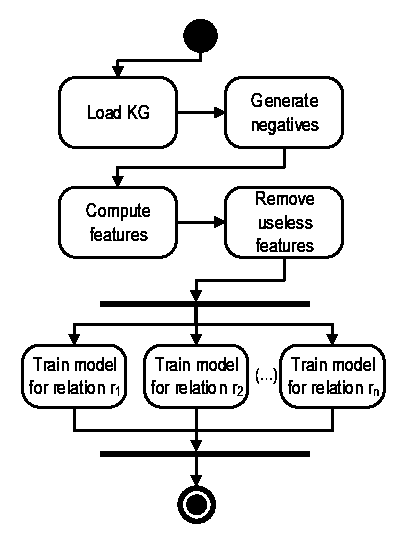
\includegraphics[width=.45\textwidth]{fig/cafe/CAFE-flow}
    \caption{Workflow of CAFE}
    \label{fig:cafe-flow}
\end{figure}

The main flow of CAFE is coordinated by the class \textit{ParallelWorker}. This class can be configured to use a certain number of threads, and then internally spawns processes to parallelize the different tasks done by CAFE. This is done by splitting the total number of triples in the KG between the different threads, since the processing of triples can be done concurrently for the most part, as shown in Figure~\ref{fig:cafe-flow}. 

The method \textit{genNegs} produces negative triples using the \textit{NegativeGenerator} class and a generation strategy, since they are necessary to train the classification models.

Then, the method \textit{compFeats} transforms every triple in the KG into a labeled feature vector, using a series of neighborhood-aware features that leverage the similarities of the neighborhoods of two entities in a KG. This is done by measuring the similarities of the entity neighborhoods of the source and target of a triple, using measures such as the Jaccard index of similarity, analyzing the size of such neighborhoods using measures such as the Adamic-Adar index; as well as assessing the overall connectivity of the entities of a triple using the N-path centrality index.

The method \textit{filtFeats} removes the features that have the same value in all labeled vectors, since they have no predictive power. Finally, method \textit{getClassifier} trains and returns a neural classifier for a given set of labeled vectors, corresponding to a certain relation in the KG. Given that the work done by these methods is usually carried out in an independent manner for each triple, it is parallelized among different execution threads.

Class \textit{ParallelWorker} uses other classes by means of composition to perform specialized tasks: Class \textit{NegativeGenerator} provides a unified interface to easily generate a negative triple in a KG following one of the available strategies, which are implemented using \textit{NegGenerationStrategy} classes.

Class \textit{KGLoader}, through its \textit{load} method, is used to read and write KGs in different formats, namely: N3, Turtle, and RDF/XML.

Class \textit{FeatureVectorCalculator} is responsible for applying the previously discussed catalogue of features to any given triple using the method \textit{getVec}, resulting in a labeled vector for that triple. The catalogue of available features can be easily expanded thanks to the \textit{Feature} class, since each individual feature is implemented as an instance of that class.

Class \textit{FeatureFilterer} specializes in removing useless features from a feature vector, i.e., those that share the same value in all vectors and thus have no predictive power. Method \textit{filtFeat} receives the labeled vector to be processed and a set of all other labeled vectors, to allow for the multithreaded processing of different labeled vectors simultaneously.

Finally, the \textit{NeuralClassifier} class produces, trains and evaluates the neural models that determine whether a triple is correct. These models receive as input the feature vector generated from the triple in question, and outputs a confidence value between 0 and 1. The models used by CAFE have three feed-forward layers with 1024, 512 and 256 neurons each. The method \textit{initialize} produces a new model for a certain relation, to allow it to specialize in the specific details of said relation, which may be different to other relations present in the KG. The method \textit{train} receives the training set of labeled vectors resulting from processing a KG with the \textit{ParallelWorker}, and uses them to train the classification model. This method uses a learning rate of 0.001, a dropout of 0.1 for all layers, a batch size of 16 and 100 epochs, as these parameters have been proven to yield satisfactory results in some of our previous work \cite{borrego2021}. Then, all vectors in the testing set are evaluated using the \textit{predict} method.

Throughout the whole process, the \textit{Settings} class is queried to retrieve the configuration parameters set by the user, e.g., the relative sizes of the training and testing splits, or the negative generation strategy to use.

CAFE has two main dependencies with external libraries: NetworkX \cite{hagberg2008networkx}, which is used to internally store the KG and apply graph-based algorithms to compute the different features; and TensorFlow \cite{tensorflow2015}, which is used to create, train and apply the neural classification models.

\subsection{Design and performance considerations}
The architecture of CAFE shares some common patterns and design decisions with that of CHAI, described in the previous chapter. Most classes only need to be instantiated once throughout the execution of CAFE and, for this reason, we have decided to turn them into singletons for simplicity of use and to minimize the use of memory.

There are, nonetheless, a number of classes that clearly must allow multiple instances of them to exist, in order to represent variations of the same concept. A prime example of this is the Feature class: all features share the same interface, since they receive a triple and the KG that contains it and produces a numeric value. However, in order to accommodate all features defined in Section~\ref{sec:cafe-features}, each one of them exists as an instance of Feature.

Another example is the possible existence of multiple negative generation strategies, where one must be chosen at runtime according to the selection of the user. In both cases, they are accessed through auxiliary classes that act as catalogues, automatically detecting and loading all instances of the catalogued classes. 

Given that CAFE is a very computationally intensive system, several optimizations have been made to make the best possible use of the resources of the system it runs on. Due to the fact that computing a feature vector for a triple can be done independently of all other triples in a KG, this task is parallelized and evenly distributed among all available cores in a CPU. This, however, comes at the cost of ensuring that all singletons in the system are thread-safe, given that they will be accessed by multiple processes at the same time.

Finally, it is important to note that all features defined by CAFE are deterministic, and will always return the same value for the same triple in a KG. Most features only analyze one of the entities in a triple at a time, and thus are re-computed very often for the same entity. For this reason, we have implemented a thread-shared caching strategy, in which the result of applying a feature to a triple is stored into a cache that is accessed by all threads. This allows CAFE to significantly reduce the number of calculations that must be performed when processing a KG.

\section{Evaluation}\label{sec:cafe-evaluation}
In this section, we present the evaluation that we carried out to assess the performance and effectiveness of CAFE. First, we introduce the Knowledge Graphs on which CAFE was applied and an overview of their main characteristics. Next, we explain the methodology that we used to evaluate CAFE. Finally, we show and discuss the results of our evaluation.

\subsection{Experimental data}
We evaluated our proposal using four KGs provided by the freely available AYNEC-DataGen~\cite{ayala2019} tool: FB13-A, WN11-AR, WN18-AR and NELL-AR. These KGs are based on the well-known FB13, WN11 \cite{socher2013}, WN18~\cite{bordes2014}, and a subset of NELL proposed in \cite{gardner2015}. However, they have been processed to remove reciprocal relations detected by AYNEC, i.e., relations $r$ and $r'$ such that, if $(s, r, t)$ exists, then $(t, r', s)$ also exists very frequently. Additionally, relations that amount to less than 5\% of the total number of triples in the graph have been removed.

These evaluation KGs originally contained one negative example per each positive triple in both their training and testing splits. In order to study how the KG completion techniques perform when presented with a much higher volume of negative evidence, we created versions of these graphs whose testing splits contained 10 negative examples per positive, using the AYNEC-DataGen tool. We believe that this is a more realistic scenario, since a much higher number of negative examples per positive triple is typically expected in real-world KG completion tasks~\cite{borrego2019}. To avoid confusion, we denote these versions as FB13-A-10, WN11-AR-10, WN18-AR-10 and NELL-AR-10.

For FB13-A-10, WN11-AR-10 and WN18-AR-10, we aimed to predict all possible relations, and for NELL-AR-10 we focused on the same subset of 10 relations that were used to evaluate SFE~\cite{gardner2015}. However, in the latter KG, one relation was removed by AYNEC for being the reciprocal of another relation, leaving 9 relations for evaluation. In the specific case of FB13-A-10, we transferred 25\% of the training triples over to the testing set in order to provide testing examples for some relations, as they were not available in the original KG as introduced in \cite{socher2013}. Table \ref{table:cafe-datasets} provides an overview of the aforementioned KGs. In the case of NELL-AR-10, we show in parentheses the amount of triples and relations that were considered for evaluation, although the entire graph was used for computing features.

\begin{table}
    % \footnotesize
    \begin{center}
    \begin{tabular}{ >{\raggedright\arraybackslash}M{3.5cm} | M{2.5cm} | M{2.5cm} | M{1.75cm} | M{1.75cm} }
    \centering \textbf{KG} & \textbf{Training triples} & \textbf{Test triples} & \textbf{Entities} & \textbf{Relations} \\
    % actualizado marzo 2021
    \hline
    FB13-A-10 & 228,172 & 481,457 & 74,998 & 13 \\ 
    \hline
    WN11-AR-10 & 77,948 & 198,231 & 38,195 & 9 \\
    \hline 
    WN18-AR-10 & 71,984 & 183,051 & 40,943 & 11 \\
    \hline 
    NELL-AR-10 & 86,971 (1,451) & 219,374 (5,083) & 53,934 & 148 (9) \\
    \end{tabular}
    \caption{Overview of the KGs used for evaluating CAFE}
    \label{table:cafe-datasets}
    \end{center}
\end{table}

\subsection{Experimental setup}
A neural prediction model was created for every relation of interest and trained using its corresponding training set. Then, the model was applied to all feature vectors in the test set, and we compared the expected label (which denotes whether it represents a correct triple or not) against the label that was produced by our model. We report our results in terms of precision, recall and F1, in order to determine how effective our proposal is when determining the correctness of a given triple.

We evaluated three versions of CAFE, denoted CAFE$_1$ to CAFE$_3$, which were limited to using feature instances that exploited neighborhood subgraphs and paths of a maximum size of 1, 2, and 3, respectively. This was done in order to study how using larger neighborhoods affects the effectiveness of CAFE.

There exist many different KG completion proposals, and they often use different evaluation metrics \cite{speranskaya2020}. Due to this, it is very difficult to perform a comparison across a large number of them in a manner that is fair and rigorous. For this reason, we used TransE~\cite{bordes2013}, TransD~\cite{ji2015}, TransH~\cite{wang2014}, TransR~\cite{lin2015}, Analogy~\cite{liu2017}, SimplE~\cite{kazemi2018} and RotatE~\cite{sun2019} as baselines for our evaluation, since they are some of the most well-known state-of-the-art KG completion proposals. In order to provide a common evaluation environment for these different proposals, we used the OpenKE \cite{han2018} framework to train and evaluate these proposals using the previously discussed Knowledge Graphs. Additionally, since these proposals usually report metrics like MRR and Precision@N, we used the utilities provided by OpenKE to obtain binary labels for the testing triples, by setting a likelihood threshold in a way that optimized the classification results.

We selected the following values for the hyperparameters of our neural models: 3 layers with 1024, 512 and 256 neurons each, learning rate of 0.001, batch size of 16, dropout of 0.1 for all layers, 100 epochs and validation ratio of 10\%. When two or more models were to be combined, we joined their results using a hidden layer with 3 neurons and an output layer with a single neuron. These values for the hyperparameters were chosen using a hold-out or ``dev'' set for the FB13-A-10 KG, and all KGs were then evaluated using the same hyperparameters. We chose them because they provided satisfactory results in our empirical tests.

All our experiments were conducted on a computer equipped with an Intel Core i9-9900K CPU, 32GB of RAM and an Nvidia RTX 2080 Ti GPU.

\subsection{Results and discussion}
In Figure \ref{fig:cafe-boxes}, we show the evaluation results for CAFE$_1$, CAFE$_2$, CAFE$_3$, and the related state-of-the-art proposals. For the sake of clarity, this Figure only displays the F1 values for each technique. Additionally, Table \ref{fig:cafe-table-results} shows the detailed results for all relations in every KG and for all metrics under evaluation.

\begin{figure}[!htp]
    \centering
    \def\subfigscale{0.6\textwidth}
    
    \subfigure[FB13-A-10]{
        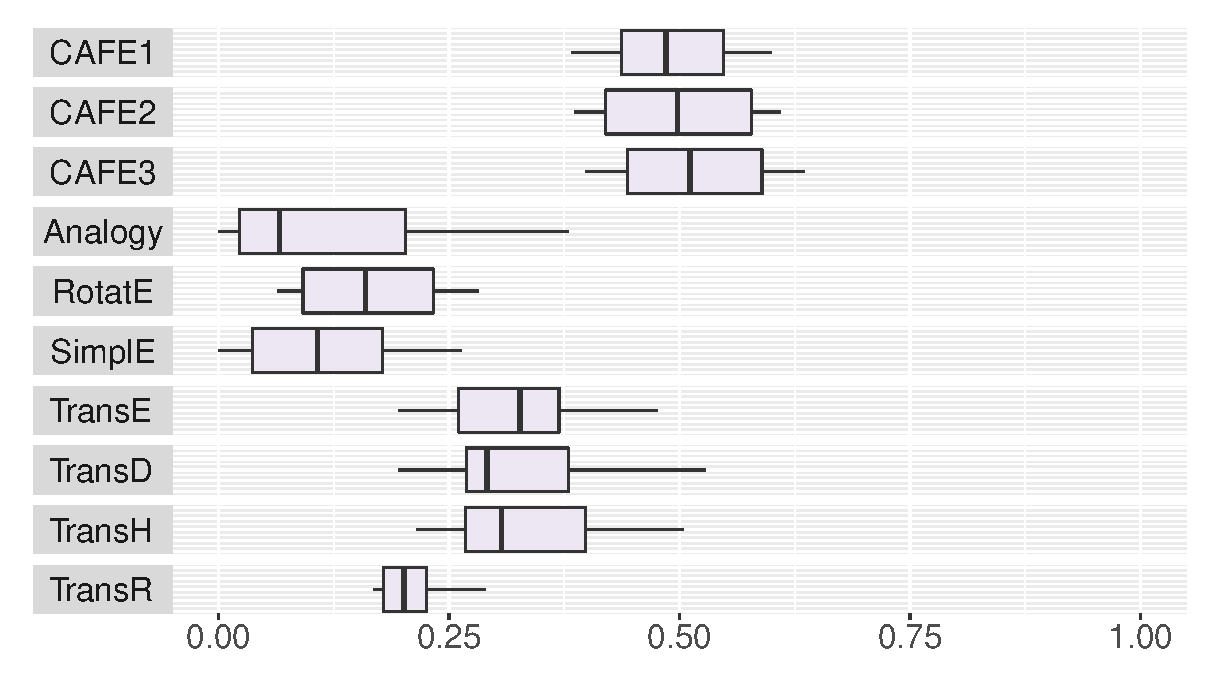
\includegraphics[width=\subfigscale]{fig/cafe/boxes/FB13-A-10}
        \label{fig:box-FB13-A-10}
    }\\
    \subfigure[NELL-AR-10]{
        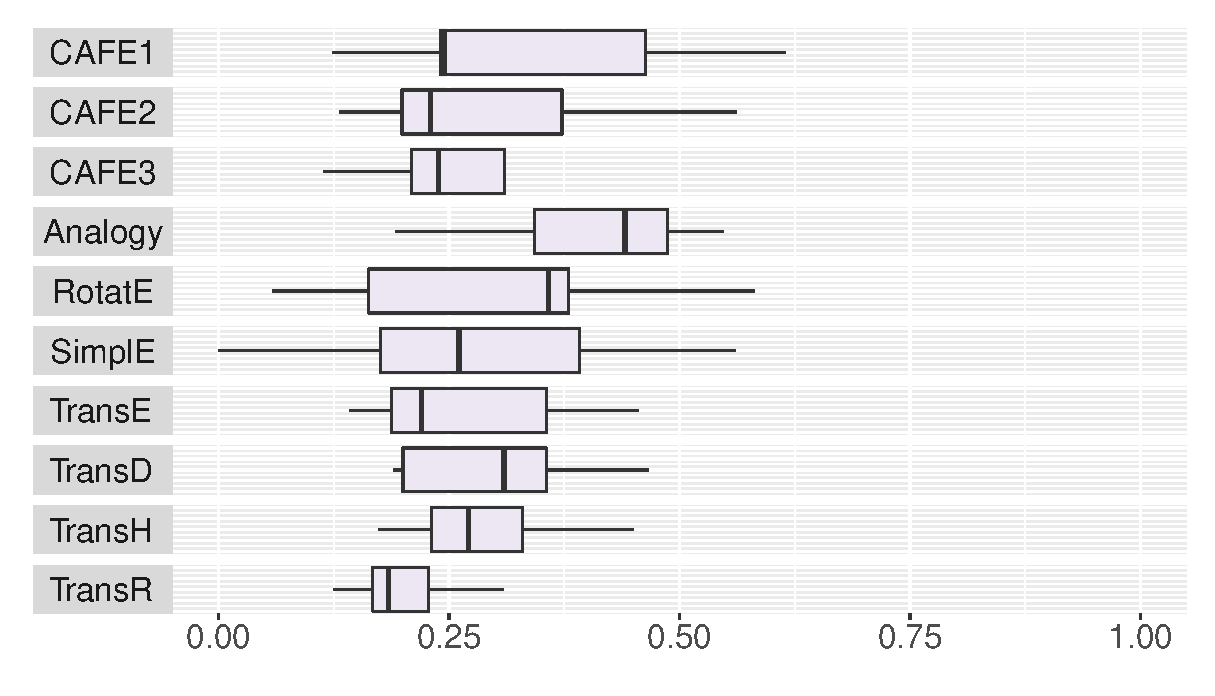
\includegraphics[width=\subfigscale]{fig/cafe/boxes/NELL-AR-10}
        \label{fig:box-NELL-AR-10}
    }\\
    \subfigure[WN11-AR-10]{
        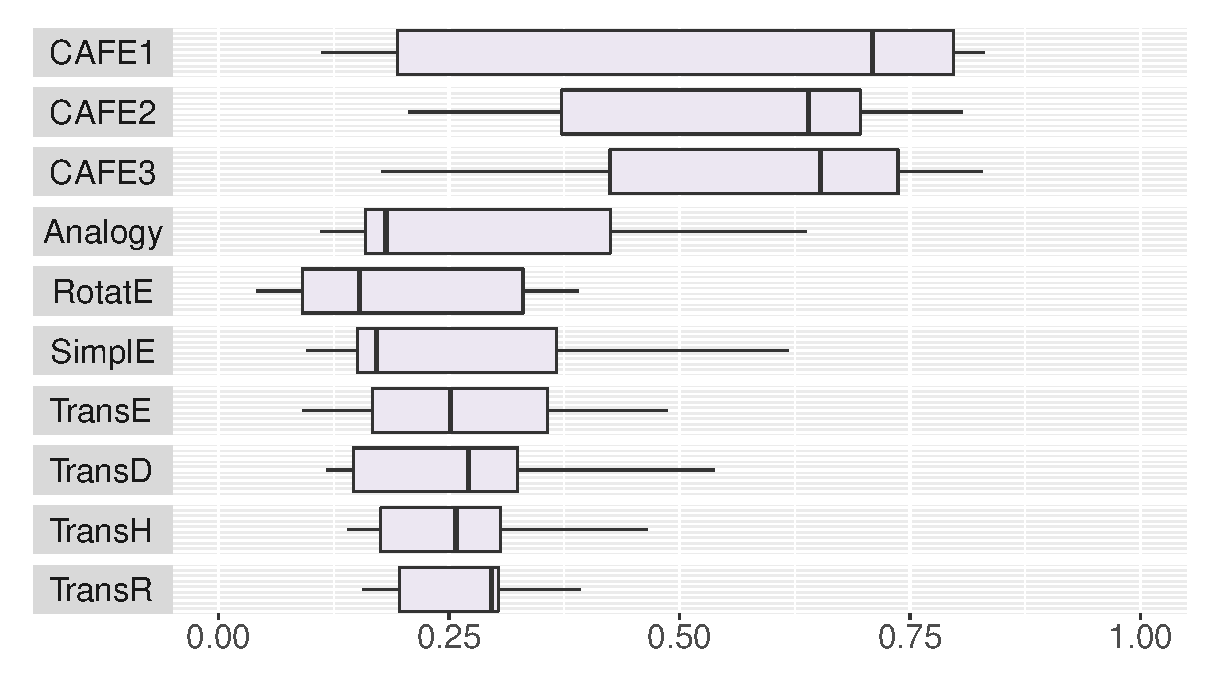
\includegraphics[width=\subfigscale]{fig/cafe/boxes/WN11-AR-10}
        \label{fig:box-WN11-AR-10}
    }

    \caption{F1 comparison between CAFE and other proposals}
    \label{fig:cafe-boxes}
\end{figure}

\begin{figure}[!htp]\ContinuedFloat
    \centering
    \def\subfigscale{0.6\textwidth}
    
    \subfigure[WN18-AR-10]{
        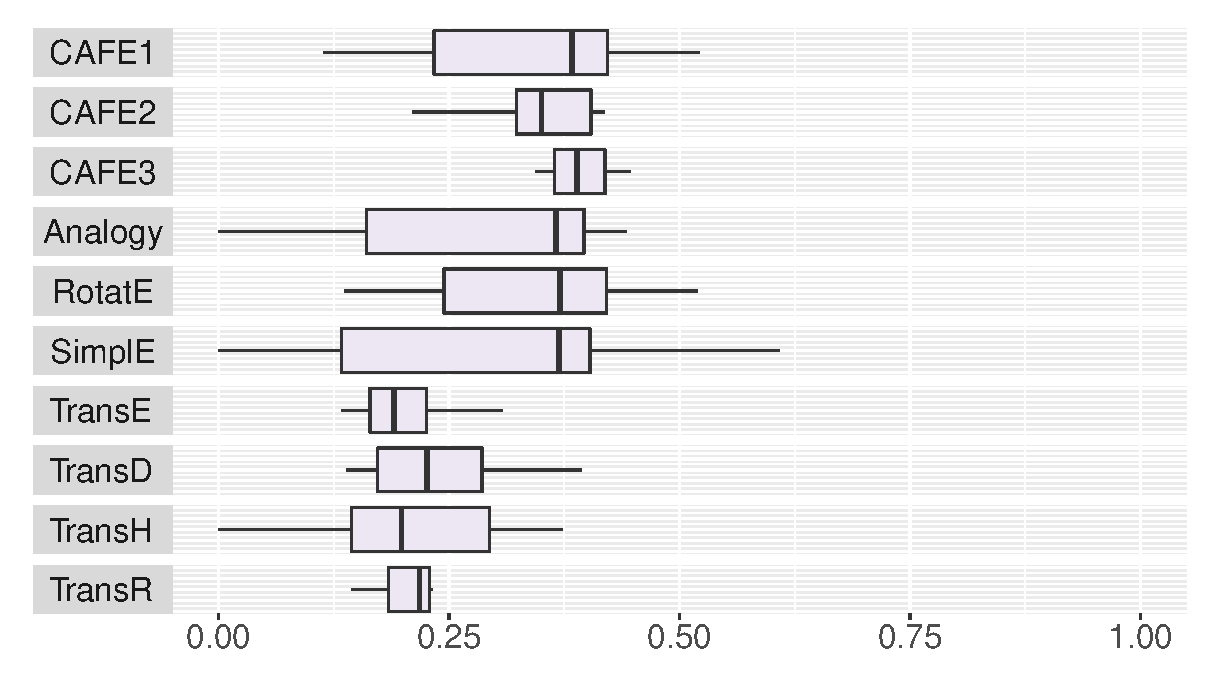
\includegraphics[width=\subfigscale]{fig/cafe/boxes/WN18-AR-10}
        \label{fig:box-WN18-AR-10}
    }\\
    
    \caption{F1 comparison between CAFE and other proposals (cont.)}
\end{figure}

\begin{figure}[!htp]
    \centering
    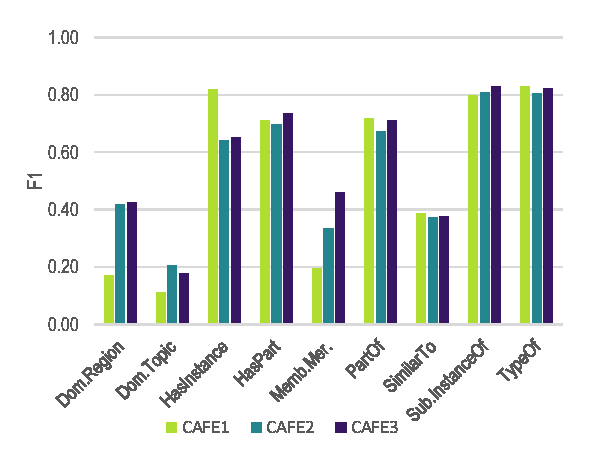
\includegraphics[width=.75\textwidth]{fig/cafe/wn11_bars}
    \caption{F1 scores in the WN11-AR-10 KG}
    \label{fig:cafe-wn11-bars}
\end{figure}

Our results show that CAFE is able to match the performance of state-of-the-art proposals, and in many cases achieve higher values on the metrics under evaluation. In the cases of FB13-A-10 (Figure \ref{fig:box-FB13-A-10}) and WN18-AR-10 (Figure \ref{fig:box-WN18-AR-10}), CAFE can reach or surpass the F1 scores achieved by other proposals in a consistent manner. CAFE also provides better results in the WN11-AR-10 (Figure \ref{fig:box-WN11-AR-10}) KG, although with a higher degree of variability, and matches the performance of the rest of the analyzed techniques in the NELL-AR-10 (Figure \ref{fig:box-NELL-AR-10}) KG. These results show that CAFE can be more effective than other proposals in challenging classification scenarios.

\newpage
\clearpage

\begin{table}[H]
    \centering
    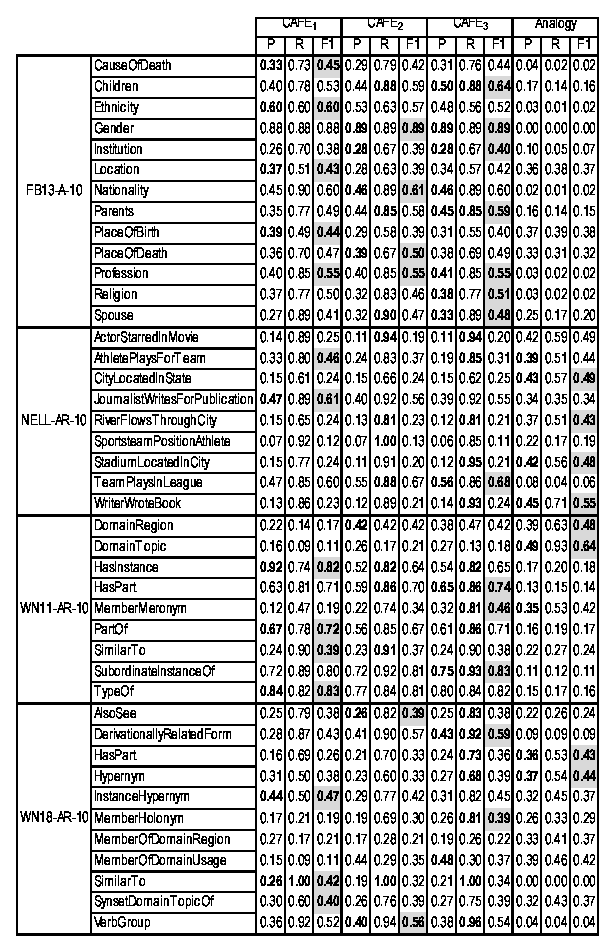
\includegraphics[height=0.8\paperheight,right]{fig/cafe/table-cafe-left}%
    \caption{Detailed CAFE results}
    \label{fig:cafe-table-results}
\end{table}  
\begin{table}[H]\ContinuedFloat
    \centering
    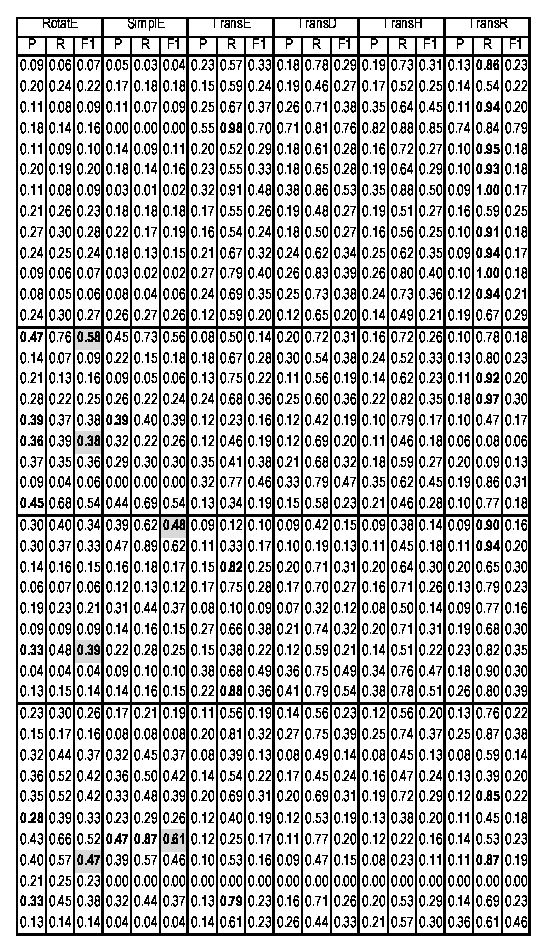
\includegraphics[height=0.8\paperheight,left]{fig/cafe/table-cafe-right}%
    \caption{Detailed CAFE results (cont.)}
\end{table}

% \afterpage{%
%     % \clearpage% flush all other floats
%     % \ifodd\value{page}
%     % %#\else% uncomment this else to get odd/even instead of even/odd
%     %     \expandafter\afterpage% put it on the next page if this one is odd
%     % \fi
%     {%
      
%     \cleardoublepage
    
%     }%
% }

\newpage

Table \ref{fig:cafe-table-results} displays that, in general, both a satisfactory precision and recall can be achieved, and thus we consider that CAFE is generally effective. However, there exists a number of relations for which a very high precision value is obtained at the expense of a lower recall or vice-versa, resulting in a typical precision-recall trade-off. We also observe that the nature of every individual relation has a significant impact in the results, since some of them are harder to predict than others. Such is the case of the relation \textit{cause\_of\_death}, since learning to predict the cause of the death of a person with a very high effectiveness would be a remarkable achievement that unfortunately falls out of the scope of this work. We further discuss this limitation in Section \ref{sec:cafe-limitations}.

Regarding the question of how using different neighborhood sizes affects the effectiveness of CAFE, Figure~\ref{fig:cafe-boxes} shows that the metrics under evaluation are generally higher for CAFE$_2$ than for CAFE$_1$, but the same cannot always be said for CAFE$_3$ and CAFE$_2$. Indeed, metrics appear to remain stagnant or even decrease when using larger neighborhoods in some cases. For example, in FB13-A-10 (Figure \ref{fig:box-FB13-A-10}), we do not observe a significant increase in effectiveness when using larger neighborhood subgraphs, which suggests that the most useful information is readily available in the immediate vicinities of the relevant entities. In the cases of WN11-AR-10 (Figure \ref{fig:box-WN11-AR-10}) and WN18-AR-10 (Figure \ref{fig:box-WN18-AR-10}), an improvement is observed when using neighborhoods of size 2, but further expanding the neighborhood size does not seem to have a significant impact. A possible conclusion for this is that, at a certain point, larger neighborhood subgraphs do not provide additional value or predictive power over smaller ones. In a worst-case scenario, the number of features with little to no predictive power would greatly increase by using larger neighborhood sizes, negatively affecting the results. This effect actually occurs in the case of the NELL-AR-10 KG (Figure \ref{fig:box-NELL-AR-10}), where effectiveness decreases when increasing the size of the neighborhood subgraphs for which we compute features. A plausible explanation for this is that it has been noted that NELL contains noisier data~\cite{paulheim2014}, and thus taking larger neighborhoods into account significantly increases the amount of noise that our classification model has to deal with, reducing its effectiveness.

\section{Limitations}\label{sec:cafe-limitations}
Despite our triple classification proposal being generally effective, it has some limitations. It does not work well for relations for which useful predictive information cannot always be found in the neighborhoods of the entities in a triple. In this regard, we identify two types of relations: those that can be predicted using other information present in the KG, and those for which the entities and relations in their neighborhoods do not provide useful information, and thus are much harder to predict. This dichotomy can be observed in the results shown in Table \ref{fig:cafe-table-results}, and it is especially notable in the WN11-AR-10 KG. For the sake of visualization, we display the results of applying CAFE to this Knowledge Graph in Figure~\ref{fig:cafe-wn11-bars}.

This difference is particularly visible in the \textit{Similar to} and \textit{Domain topic} relations, which have low F1 scores. Upon manual inspection, we found that \textit{Similar to} tends to link words that are generally isolated within the KG and share very little common context. Also, \textit{Domain topic} is extremely broad, causing the two entities in a triple to have few or no relevant common elements in their neighborhoods, e.g., (\textit{Britain}, \textit{Domain topic}, \textit{Surgery}).

In other cases, even if some information is present in the neighborhoods under consideration, it may be not successfully captured by CAFE due to the large amount of irrelevant data surrounding it. In this regard, the NELL-AR-10 KG shows that larger neighborhood sizes are not always better for predictive purposes, since the amount of noise they may include can be detrimental for the performance of CAFE. This can be due to some source or target entities being present in many triples (for example, countries). Therefore, larger neighborhoods of these entities introduce many other entities that are not relevant to the triple under evaluation. In these cases, it is up to the users to decide which maximum neighborhood size best caters to their interests.

\section{Summary}\label{sec:cafe-summary}
In this chapter we have introduced CAFE, our proposal to classify candidate triples for Knowledge Graph completion. CAFE defines a set of neighborhood-aware features which evaluate several aspects of a triple, by checking for shared neighborhoods at several distances with other triples in a KG, and then combines the values of all features into a feature vector. Once all candidate triples have been transformed into feature vectors, CAFE trains and applies a neural binary classifier to discern between correct and incorrect triples, and provides the user with a set of correct candidate triples to add back to the KG. Our experimental evaluation shows that CAFE is very effective, outperforming other state-of-the-art approaches in a number of well-known Knowledge Graphs of different sizes and domains.

    \chapter{SciCheck: Completing scientific Knowledge Graphs}\label{chap:scicheck}

\chapterQuote{
    \hfill
    \foreignlanguage{russian}{\sffamily доверяй, но проверяй.}\\
    \null
    \hfill
    \textit{(Trust, but verify.)}
}{--- Russian proverb}

\chapterAbstract{S}{cientific knowledge is in constant expansion, and many efforts have been developed throughout the years to capture it in a structured format. Knowledge Graphs can support this task, by linking entities representing research concepts together. These scientific KGs have particular nuances that make completing them a particularly challenging task. In this chapter, we introduce SciCheck, our proposal to complete Knowledge Graphs representing research concepts. This chapter is structured in the following manner: Section~\ref{sec:sci-intro} provides an introduction, Section~\ref{sec:sci-proposal} describes SciCheck in detail, including the features that it uses to characterize triples representing scientific knowledge, Section~\ref{sec:sci-evaluation} presents the experimental evaluation that we have carried out to assess its efficacy and efficiency in practice, Section~\ref{sec:sci-aikg} shows a practical application of SciCheck on AI-KG, a large-scale Knowledge Graph of research concepts and, finally, Section~\ref{sec:sci-summary} provides a summary of the chapter.}

\section{Introduction}\label{sec:sci-intro}
In recent years, we have witnessed the appearance of a number of Knowledge Graphs that represent research and scientific knowledge. These graphs are generally either manually curated~\cite{jaradeh2019, bodenreider2004, kuhn2016}, or constructed automatically from academic metadata~\cite{dessi2020aikg, salatino2020, rossanez2020}. However, just like most KGs, they suffer from incompleteness, which means that some well-known scientific knowledge may not be present in them.

This chapter introduces SciCheck~\cite{borrego2022}, our proposal to complete scientific Knowledge Graphs. SciCheck extends our generic triple classification technique, CAFE, by adding a number of features and heuristics specifically tailored for the scientific domain. SciCheck is able to compute a confidence score for every triple representing a scientific claim, and then derive a binary classification for it based on its confidence. Similarly to CAFE, SciCheck works by transforming a triple into numeric features, but includes additional heuristics to immediately discard incorrect scientific triples.

We evaluate the efficacy of SciCheck on seven different Knowledge Graphs and against nine alternative approaches to this task. Our evaluation shows that SciCheck is able to obtain a significantly better precision than its state-of-the-art counterparts, which is of the essence to reliably extend scientific Knowledge Graphs.

Additionally, we used SciCheck to extend the Artificial Intelligence Knowledge Graph (AI-KG)~\cite{dessi2020aikg}, a large-scale open KG that is constructed automatically using the 300K most cited papers in the field of Artificial Intelligence. Initially, AI-KG contained 1.2M statements about scientific claims in this field. By applying SciCheck to it, we have expanded it with 300K additional high-confidence statements. This application has resulted in the release of a new, expanded version of AI-KG, as well as in the creation of two high-quality Knowledge Graphs that can be used to benchmark KG completion.

\section{Our proposal}\label{sec:sci-proposal}
SciCheck is a triple classification technique specifically designed to complete scientific statements in a Knowledge Graph. It is an extension of the CAFE approach~\cite{borrego2021} that incorporates a new set of features and heuristics that are specifically tailored to capture scientific knowledge. 

SciCheck takes an entire KG in the form of triples as input, and produces one neural-based classifier for each relation in the KG as output. Specifically, given a relationship $r$, SciCheck generates a model $f_r : (s,r,t) \rightarrow c$, that assigns a confidence score $c$ in the range $[0,1]$ to any arbitrary triple $(s,r,t)$ to solve a binary classification task (``is the triple correct or not?''). To feed the models, triples are converted into a numerical vector representation using ad-hoc features and contextual embedding representations. SciCheck can operate on any KG and focuses on optimizing precision, to ensure that the knowledge deemed correct is trustworthy.

In the following, we describe and discuss the features that SciCheck uses to characterize a triple in the context of a scientific KG.

\begin{figure}[!htp]
    \centering
    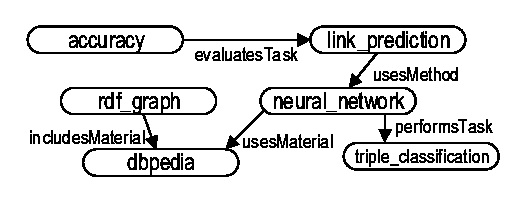
\includegraphics[width=.55\textwidth]{fig/scicheck/example_kg}
    \caption{A small KG with research information about the Semantic Web}
    \label{fig:example-kg-sw}
\end{figure}

For the sake of illustration, Figure \ref{fig:example-kg-sw} displays a small KG that will be used to provide specific examples.

\subsection{Extended feature set}
SciCheck uses an extensible set of features specifically made to capture and process scientific information, which represent the neighborhoods of the two entities of a triple in a variety of ways. Each triple is evaluated by all features. Additionally, each feature can also depend on a number of parameters, such as a maximum neighborhood size. 

Since, as described, SciCheck is an extension of CAFE, we enumerate only the additional features that it incorporates with respect to the original CAFE approach.

% \scifeature
% {Number of entities in the neighborhood of size $n$ of the source and the target of a triple} 
% {For example, in Figure \ref{fig:example-kg-sw}, three entities can be reached in total using up to two hops from \textit{link\_prediction}, namely, \textit{neural\_network}, \textit{dbpedia}, and \textit{triple\_classification}. Note that the entity \textit{accuracy} is not present in the neighborhood because of the directionality of the edges.} 

% \scifeature
% {Index of N-path centrality \cite{thakara2011} of the source and target of a triple}
% {This feature assesses how well-connected an entity is to the rest of the graph in relative terms. It is defined as follows: for every vertex $v$ of a generic graph $G=(V,E)$, the $n$-path centrality $C_k(v)$ is defined as the sum, over all possible source nodes $s$, of the probability that a message originating from $s$ goes through $v$, assuming that the message traversals are only going along random simple paths of at most $k$ edges. For example, in the KG shown in Figure \ref{fig:example-kg-sw}, the entity \textit{dbpedia} has a higher N-path centrality than \textit{accuracy}, since a random path from any entity in the graph is more likely to go through the former than the latter, considering the directionality of the graph.}

% \scifeature
% {Cardinality of the intersection of the neighborhoods of size $n$ of the source and target of the triple}
% {This feature measures the raw amount of common entities in the vicinities of the two entities in a triple. For example, using a size $n = 1$ in the example shown in Figure \ref{fig:example-kg-sw}, the entities \textit{rdf\_graph} and \textit{neural\_network} have the common entity \textit{dbpedia} in their neighborhoods.}

% \scifeature
% {Jaccard index of the neighborhoods of size $n$ of the source and target of the triple}
% {This feature provides a similar assessment as the previous one, but normalized in the interval $[0, 1]$.}
% The Jaccard index is defined as:
% \[
%     J(A,B)=\frac{|A \cap B|}{|A \cup B|}
% \]

% \scifeature
% {Adamic-Adar index \cite{adamicadar2003} between the source and target of the triple}
% {This index gives higher scores to entities whose neighborhoods are smaller. It complements the previous two features, since a higher number of shared nearby entities is likely to be less significant if the source and target have a very large amount of connections. It is defined as the sum of the inverse logarithmic degree centrality of the neighbors shared by the two nodes,
% \[
%     A(x,y) = \sum_{u \in N(x) \cap N(y)}\frac{1}{log|N(u)|}
% \]

% \noindent where $N(u)$ is the set of nodes adjacent to $u$.}

% \scifeature
% {Paths of length $r$ between the source and target entities}
% {For example, in Figure~\ref{fig:example-kg-sw}, the entities \textit{link\_prediction} and \textit{dbpedia} are connected by a path of length 2, by means of the triples \textit{(link\_prediction, usesMethod, neural\_network)} and \textit{(neural\_network, usesMaterial, dbpedia)}. Additionally, the relations that are present in those paths are also encoded using a $r$-hot vector.}

\scifeature
{Cosine similarity of the word embeddings of the source and target entities}
{This feature measures the semantic similarity of the two entities in a triple, using any entity embeddings. If we consider $A$ and $B$ to be the embeddings of the source and target entities of the triple respectively, it is defined as:}
        
\[
    \cos (A, B) = 
    \frac{ \sum_{i=1}^{n}{{A}_i{B}_i} }{ \sqrt{\sum_{i=1}^{n}{({A}_i)^2}} \sqrt{\sum_{i=1}^{n}{({B}_i)^2}} }
\]

\scifeature
{Dot product of the word embeddings of the source and target entities}
{This feature complements the previous one by also taking into account the magnitudes of the embeddings of the entities. If we consider $A$ and $B$ to be the embeddings of the source and target entities of the triple respectively, it is defined as:}

\[
    A \cdot B = \sum_{i=1}^{n}{A_i B_i}
\]

\newpage

\scifeature
{Types of the source and target entities according to the ontology of the Knowledge Graph}
{This feature encodes the known types of the entities according to the available ontology as two one-hot vectors. In Figure \ref{fig:example-kg-sw}, the entity \textit{dbpedia} is of type \textit{Resource}, while \textit{accuracy} is a \textit{Metric}.}

% $f_1$ and $f_2$ leverage the fact that large neighborhoods are more prone to contain unrelated information, while smaller ones are usually more specific. This is especially true in the scientific domain, since, as an example, the entity \textit{neural\_network} may be mentioned in a large amount of papers and proposals that are not directly related to each other.

% The features that measure the similarities of two neighborhoods ($f_3$, $f_4$, and $f_5$) follow the intuition that correct triples have a higher amount of shared entities in their respective neighborhoods than incorrect ones, as shown by previous research~\cite{vahdati2016, borrego2021, dessi2021assessment}.

% Feature $f_6$ measures the number of paths between two entities because a correct triple will typically have a larger number of unique paths of a given maximum length between its source and target entities than an incorrect one. Furthermore, the information about which relations are comprised by those paths can be useful since the semantic meaning of a path changes depending on the relevant relations. 

Regarding the rationales of the new features, $f_1$ incorporates information from the word embeddings of the two entities, which have been shown to be advantageous for triple classification \cite{sun2019, kazemi2018}. SciCheck uses by default the \roberta{} model \cite{liu2019roberta} to generate the word embeddings, since is able to capture and represent semantic similarities across a wide range of domains. Similarly, $f_2$ provides a similar assessment, but uses the magnitudes of the embedding vectors to extract additional information from them.

Feature $f_3$ leverages the ontological schema of the KG. This allows SciCheck to include information regarding the types of the two entities in a triple into the feature vector for that triple. Furthermore, SciCheck can automatically classify a triple as incorrect if the triple does not respect the domains and ranges of the relation as defined in the ontological schema. For example, in the KG shown in Figure~\ref{fig:example-kg-sw}, the triple \textit{(accuracy, evaluatesTask, rdf\_graph)} would be considered incorrect without further evaluation, because the range of the relation \textit{evaluatesTask} is the type \textit{Task}, while \textit{rdf\_graph} is a \textit{Material}. 

This extension of the set of features allows SciCheck to better characterize scientific entities and predicates. In particular, the features based on word embeddings enable SciCheck to exploit the implicit contextual information from the training papers that may not be encoded in the KG.
Additionally, the inclusion of ontology-based features allows SciCheck to take advantage of the available high-level knowledge about any specific domain. These improvements are particularly crucial for assessing scientific claims, which tend to use a specific jargon and to rely on a well-defined epistemological framework.

Furthermore, different types of relations in the graph may carry specific insight that should be captured separately. For this reason, SciCheck first computes all features in the input KG as-is, and then it computes them again in different versions of the KG where only relations of a single type are present. This is done for all the different relations in the KG. Additionally, in features that use the neighborhoods of the source and target entities, such as those originally defined by CAFE, these two neighborhoods are calculated using all possible combinations of relations. Finally, SciCheck concatenates all the resulting features in the final feature vector. The features which involve computing entity neighborhoods or paths use a maximum neighborhood size for their computations. Following the findings in \cite{borrego2021}, by default SciCheck computes them for a maximum size of 1, 2, and 3. The resulting set of features using different neighborhood sizes are eventually all added to the final feature vector. %Considering all the possible combinations with the number of different relations in the graph, which also affects the size of the feature vector as described previously, the number of total features is $num_{hops} \times 6 \times \#rels^2$ + $3 \times \#rels$, where $\#rels$ is the number of distinct relations in the KG.

% \subsection{Workflow}
% \todo[inline]{Hablar aquí por encima del workflow, hacer un diagramita que no se parezca mucho al de CAFE}

\section{Evaluation}\label{sec:sci-evaluation}
In this section, we describe the experimental setup that we devised to test the effectiveness of SciCheck in practice. First, we introduce a number of similar state-of-the-art approaches to triple classification that serve as baselines for our evaluation. Next, we present the KGs that we used to validate our proposal. Finally, we show and discuss the results of our evaluation.

\subsection{Baselines}
We evaluated the performance of SciCheck against a number of alternative approaches. Five of the baselines are well-known embedding-based KG completion techniques: \textit{TransE}~\cite{bordes2013}, \textit{TransD}~\cite{ji2015}, \textit{TransH}~\cite{wang2014}, \textit{SimplE}~\cite{kazemi2018}, and \textit{ComplEx}~\cite{trouillon2016}. To provide a common ground to train and test these techniques, we used the OpenKE \cite{han2018} tool.

In order to better assess the contributions of the different components of SciCheck, we also considered five alternative versions of our approach:

\begin{itemize}
    \item \textit{CAFE Baseline}, which uses solely the context-aware features for KG completion such as neighborhood size, shared entities and connectivity from the original CAFE implementation \cite{borrego2021}.\\
    
    \item \textit{CAFE+\roberta}, which extends CAFE by considering features based on the similarity of the embeddings of the source and target entities, using the RoBERTa model.\\
    
    \item \textit{CAFE+SciBERT}, which extends CAFE by considering features based on the similarity of the embeddings of the source and target entities, using SciBERT, an alternative BERT-based text embedding model~\cite{reimers2019} specifically tailored to scientific documents.\\
    
    \item \textit{CAFE+Ontology}, which extends CAFE by considering features that identify the types of the source and target entities according to the domain ontology and also filters triples whose entities are not consistent with the domain and range restrictions of the relation.\\
    
    \item \textit{SciCheck}, the full version of our approach, which incorporates both features based on word embeddings and features based on the ontology of the Knowledge Graph.
\end{itemize}

To predict the correctness of a triple using SciCheck, we convert its confidence score in the interval $[0, 1]$ into a binary label by setting a confidence threshold for a correct triple of 0.5, as suggested in~\cite{borrego2021}. The thresholds of the other state-of-the-art techniques under evaluation and their results were obtained using the OpenKE tool, allowing it to choose the optimal value for each one.

\subsection{Evaluation data}
The previously discussed baselines were evaluated on the following Knowledge Graphs, whose characteristics are summarized in Table~\ref{table:sci-dsets}:

\begin{table}[!htp]
    % \footnotesize
    \begin{center}
    \begin{tabular}{ >{\raggedright\arraybackslash}M{2.5cm} | M{1.75cm} | M{1.75cm} | M{1.5cm} | M{1.5cm} }
    \hline\rule{0pt}{12pt}
    \textbf{KG} & \textbf{Training triples} & \textbf{Test triples} & \textbf{Entities} & \textbf{Relations} \\
    
    \hline%
    AIKG-1M & 860,512 & 430,280 & 820,708 & 20 \\ 
    AIKG-500 & 860,512 & 500 & 228 & 7 \\ 
    FB13 & 228,172 & 105,509 & 74,998 & 13 \\ 
    WN11 & 77,948 & 36,042 & 38,195 & 9 \\
    WN18 & 71,984 & 33,282 & 40,943 & 11 \\
    WN18RR & 86,835 & 3,134 & 40,943 & 11 \\
    NELL & 86,971 & 40,104 & 53,934 & 148  \\ \hline
    \end{tabular}
    \caption{Overview of the KGs used for evaluating SciCheck}
    \label{table:sci-dsets}
    \end{center}
\end{table}
    

\begin{itemize}
    \item \textit{AIKG-1M}, a new KG that we created from AI-KG. We used a de-reified version of AI-KG, in order to consider only triples which involve tasks, methods, materials, metrics, and other scientific entities. As a result, 1,075,652 triples were directly generated from scientific literature, without considering facts that were materialized using the domain semantics defined in the AI-KG ontology (e.g., transitivity). Triples were split into a training and a testing set with a split ratio of 80\%-20\%, respectively.
    To generate negative triples in the testing split, each positive triple was corrupted once by randomly replacing the target entity with another one within the domain of the relation in the triple, i.e., if the range of the target entity is a Task, then it is substituted by another entity whose type is Task. We also make sure that the randomly generated negative triple is not already present in the KG, to prevent creating false negatives whenever possible. As an example, the triple \textit{(dbpedia, usesOtherEntity, sparql\_query)} is correct, while the corrupted version \textit{(dbpedia, usesOtherEntity, cost\_function)} is considered incorrect, where \textit{sparql\_query} and \textit{cost\_function} are both of type \textit{OtherEntity}. However, negative examples were not generated for the training split, as specific KG completion techniques usually have a preferred way to generate them automatically \cite{borrego2019}. In total, the training split comprised 860,512 positive triples and the testing split includes 430,280 triples ($50\%$ positive and $50\%$ negative).\\

    \item \textit{AIKG-500}, a new KG that we constructed by manually annotating triples in AI-KG about the Semantic Web. 
    To construct it, we randomly selected 250 triples which had as their source entity one of the 24 sub-topics of the Semantic Web according to the CSO ontology \cite{salatino2020CSO} and were considered to be correct by at least 2 methods among \textit{TransE}, \textit{TransD}, \textit{TransH}, \textit{SimplE}, \textit{ComplEx}, and \textit{SciCheck}. Another 250 triples were randomly selected out of those deemed incorrect by at least 2 of the previously mentioned techniques. The resulting 500 triples were manually annotated by five domain experts, with an inter-reviewer agreement of 0.61 (according to Cohen's kappa), which is typically considered a substantial agreement.
    A majority vote approach was used to determine that 221 triples were correct and 279 were incorrect. Since this Knowledge Graph was created for the purpose of providing a small but high-quality and  manually-annotated testing split, in this evaluation we used AIKG-1M for the training split.\\

    \item \textit{FB13} \cite{socher2013}, a subset of FreeBase~\cite{bollacker2008} that focuses on relevant people and their family relations, locations, professions, and other personal data.\\
        
    \item \textit{WN11} \cite{bordes2013}, a subset of WordNet centered around different semantic relations between over 38K words.\\
        
    \item \textit{WN18} \cite{bordes2014}, which expands WN11 with additional relations.\\
    
    \item \textit{WN18RR} \cite{dettmers2018}, which improves WN18 by removing reciprocal relations in the test set. This makes triple classification more challenging, since otherwise the model can predict that a triple \textit{(a, hasChildren, b)} is true whenever the triple \textit{(b, hasParent, a)} appears in the training set.\\
        
    \item \textit{NELL} \cite{gardner2015}, a subset of the NELL KG~\cite{mitchell2018} with information and relations about many different domains, e.g., actors which starred in movies, writers and their works, or athletes and their teams.\\
\end{itemize}

It is well-known \cite{dettmers2018} that these traditional KGs suffer from information leakage between the training and test sets, due to the presence of reciprocal relations. For this reason, we removed all reciprocal relations in all KGs except WN18, since we also include its previously discussed sanitized version, WN18RR.

\subsection{Results and discussion}\label{sec:sci-results}
Table~\ref{fig:sci-table_p} and Table~\ref{fig:sci-table_r} report the precision and recall of the KG completion techniques on AIKG-1M. The results show that all CAFE-based variants outperform embedding-based techniques in precision, achieving notably higher values. Including features from the text embeddings also provides an important improvement over the base version of CAFE. Both SciCheck and the variants that improve the baseline using embedding-based features rank consistently among those with the highest precision for all relations, with the differences between them being very narrow.

\begin{figure}[!h]
    \centering
    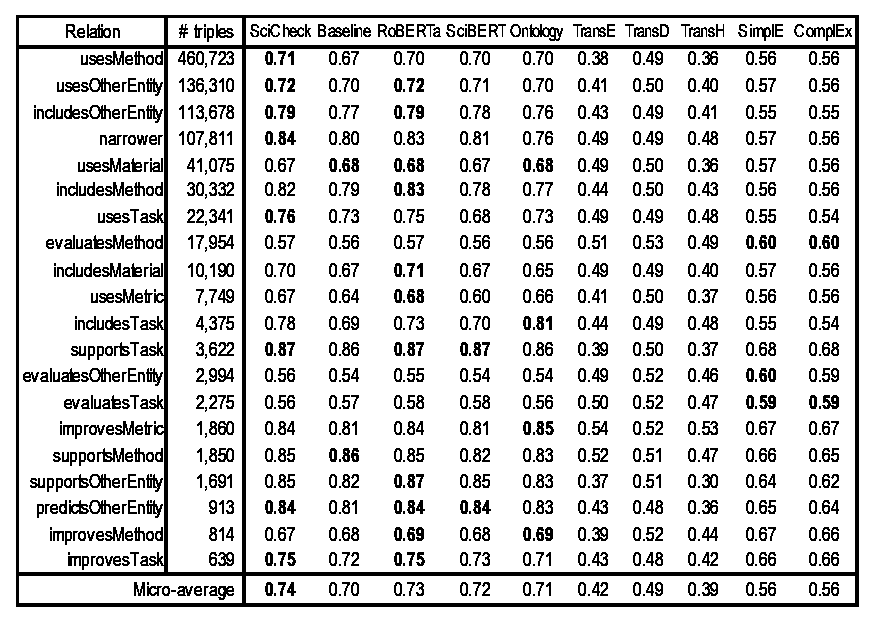
\includegraphics[width=\textwidth]{fig/scicheck/table_p}
    \captionof{table}{Precision values for SciCheck in AIKG-1M}
    \label{fig:sci-table_p}
\end{figure}

\begin{figure}[!h]
    \centering
    \includegraphics[width=\textwidth]{fig/scicheck/table_r}
    \captionof{table}{Recall values for SciCheck in AIKG-1M}
    \label{fig:sci-table_r}
\end{figure}

The best performing method in terms of precision is the full version of SciCheck (0.74), followed by CAFE+\roberta{} (0.73), which can obtain better precision for some less common relationships. 
Interestingly, using text embeddings trained specifically on academic abstracts (SciBERT) yields a slightly worse performance than using the generic \roberta{} model. This may suggest that more general embeddings may sometimes produce better performance on KGs of research concepts, but this needs to be investigated further.

The \textit{Ontology} variation, which includes one-hot type vectors and domain/range checking for the relation, only slightly improves the baseline. This is most likely due to the type-constrained way in which the negative triples were generated, since it already guarantees that the domain and range types of the relation are preserved.

The recall of SciCheck is naturally lower than that of the embedding-based approaches, in a typical precision-recall trade-off. However, this is acceptable since the main goal is to expand scientific Knowledge Graphs with correct triples, hence, a high precision is desirable. SciCheck also has a generally higher recall than all other CAFE variants. Consequently, the results suggest that SciCheck is the best performing technique for the task of reliably completing scientific Knowledge Graphs.

It is noteworthy that different relations can lead to very different performances. For instance, relations such as \textit{narrower}, \textit{supportsTask} and \textit{supportsMethod} yield very good performance. Conversely, the methods under evaluation did not perform as well on relations such as  \textit{evaluatesTask} and \textit{evaluatesOtherEntity}. This may depend on the number of relevant examples or the fact that some relations are inherently harder to predict.

In order to study the performance of the different techniques for all possible threshold values, we also report their corresponding ROC curves in Figure~\ref{fig:sci-rocs}. This analysis confirms the previous findings:  

\begin{itemize}
    \item SciCheck outperforms all other methods under evaluation.
    \item Text embedding-based features significantly improve the baseline state-of-the-art methods.
    \item Ontology-based features provide slight further improvements.
\end{itemize}

In addition, Figure~\ref{fig:sci-rocs-embs} confirms that SciCheck outperforms the standard state-of-the art methods regardless of the threshold.

\begin{figure}[!htp]
    \centering
    \def\subfw{0.45\textwidth}
    
    \subfigure[SciCheck variants]{
        \includesvg[inkscapelatex=false, width=\subfw]{fig/scicheck/roc_cafes.svg}
        \label{fig:sci-roc-cafes}
    }~
    \subfigure[SciCheck and embedding techniques]{
        \includesvg[inkscapelatex=false, width=\subfw]{fig/scicheck/roc_embs.svg}
        \label{fig:sci-rocs-embs}
    }
    
    \caption{ROC curves of the different methods on AIKG-1M}
    \label{fig:sci-rocs}
\end{figure}

To check whether the differences between the methods were statistically significant, we used DeLong's test~\cite{delong1988} to compare the areas under two curves. The p-values obtained when comparing the ROC  curve of SciCheck with the alternative methods in Figures~\ref{fig:sci-roc-cafes} and~\ref{fig:sci-rocs-embs} were all~$<0.0001$. This very high statistical confidence is due to the large number of observations, since the testing set of AIKG-1M includes more than 400,000 triples.

Table~\ref{fig:sci-table_sw} shows the performance of the methods on AIKG-500, which are consistent with the previous findings. For the sake of brevity, here we do not report the results of all CAFE variants, which are in line with those obtained on AIKG-1M. Even in a smaller, manually annotated Knowledge Graph, SciCheck achieves a high precision, which confirms that it is suitable for completing scientific Knowledge Graphs. 

\begin{figure}[!htp]
    \centering
    \includegraphics[width=\textwidth]{fig/scicheck/table_sw}
    \captionof{table}{Precision and recall values for AIKG-500}
    \label{fig:sci-table_sw}
\end{figure}

Table~\ref{fig:sci-table_kgs} reports the performance of all the techniques on five standard KGs for triple classification. The results show that SciCheck is able to outperform other techniques in almost all cases, thus being an effective triple classification tool for KGs of many different natures. They also confirm that completing scientific KGs is indeed a challenging task that requires specialized techniques, as the general-purpose embedding-based approaches yield worse results on KGs extracted from AI-KG in comparison to generic ones.

\begin{table}[!htp]
    \centering
    \includegraphics[width=.85\textwidth]{fig/scicheck/table_kgs}
    \captionof{table}{Micro-average precision and recall on four general KGs}
    \label{fig:sci-table_kgs}
\end{table}

In order to assess the scalability of our solution, Table~\ref{table:sci-times} reports the seconds used by SciCheck to process the previously discussed graphs. To ensure statistical significance, we measured the runtime for each KG 10 times, and we report the average and the standard deviation for each one. 

\begin{table}[!htp]
    % \footnotesize
    \begin{center}
    \begin{tabular}{ M{2.5cm} | M{3.5cm} }
    \hline\rule{0pt}{12pt}
    \textbf{KG} & \textbf{Runtime}  \\
    
    \hline%
    AIKG-1M & 2,758.79 $\pm$ 37.27 \\ 
    AIKG-500 & 1,794.94 $\pm$ 12.58 \\ 
    FB13 & 9,400.10 $\pm$ 63.04 \\ 
    WN11 & 34.30 $\pm$ 0.28 \\
    WN18 & 55.59 $\pm$ 0.45  \\
    WN18RR & 26.00 $\pm$ 0.14 \\
    NELL & 4.33 $\pm$ 0.09 \\ \hline
    \end{tabular}
    \caption{SciCheck runtimes in seconds for all KGs (avg $\pm$ std)}
    \label{table:sci-times}
    \end{center}
\end{table}

Table \ref{table:sci-times} shows that the runtime ranges from a few seconds to over two hours according to the specific Knowledge Graph. These differences are caused by mainly two factors. First, the amount of distinct entities corresponds directly to the number of \roberta{} embeddings that have to be computed, which are typically quite time-consuming. Hence, a larger number of entities has a negative impact on runtime. Second, and most importantly, the specific topology of every KG affects the size of the neighborhoods of the entities, and thus also affects the time it takes to compute features on them. The case of FB13 is particularly noteworthy since, in contrast with the other KGs, it contains many entities with a very high cardinality. This causes the sizes of the entity neighborhoods to grow exponentially in size, resulting in longer runtimes.

Finally, in order to provide some insights on how these times compare to other state-of-the-art approaches, Table~\ref{table:sci-times-comp} reports their runtime in seconds compared to that of SciCheck for AIKG-1M.

\begin{table}[!htp]
    % \footnotesize
    \begin{center}
    \begin{tabular}{ M{2.5cm} | M{3.5cm} }
    \hline\rule{0pt}{12pt}
    \textbf{Technique} & \textbf{Runtime}  \\
    
    \hline%
    SciCheck & 2,758.79 \\ 
    TransE & 7,147.52 \\ 
    TransD & 13,871.79 \\ 
    TransH & 10,134.41 \\
    SimplE & 6,592.20 \\
    ComplEx & 11,767.73 \\ \hline
    \end{tabular}
    \caption{Runtime comparison on AIKG-1M}
    \label{table:sci-times-comp}
    \end{center}
\end{table}
    

Embedding-based KG completion approaches were run using $1,000$ iterations, as it is commonly done in related literature~\cite{bordes2013, trouillon2016, kazemi2018, ji2015}. 
SciCheck took considerably less time to run on the large AIKG-1M KG than its state-of-the-art counterparts. This suggests that it is able to complete scientific facts in a reasonable amount of time, thus making it efficient for its application to large-scale scientific Knowledge Graphs.

\section{Practical application: AI-KG}\label{sec:sci-aikg}
One practical application of SciCheck is the advancement and expansion of AI-KG~\cite{dessi2020aikg}, a comprehensive Knowledge Graph that encompasses information about research entities in the AI field. When it was introduced in late 2020, it contained roughly 14 million RDF triples and 1.2 million reified statements related to 800,000 entities extracted from 333,000 articles about AI. It defines 5 categories of entities (tasks, methods, materials, metrics, and others) connected by 27 relations (e.g., usesMaterial, evaluatesMethod, or supportsTask). The triples in AI-KG illustrate the associations between two entities based on their joint appearances in a group of scientific papers, for instance, \textit{(sentiment\_analysis, usesMaterial, twitter\_data)}.

It should be emphasized that, in the context of AI-KG, the correctness of a triple depends on the content of its associated papers, i.e., a triple connected to a group of papers is considered to be true if said papers contain that statement. As a result, triples in AI-KG are constructed to represent particular statements made by researchers. For instance, the entity \textit{sentiment\_analysis} only captures the notion of sentiment analysis that existed in the original corpus of scientific articles on which AI-KG was built, and does not attempt to encompass all existing techniques for analyzing emotions and sentiments that are present, or under research, nowadays. A complete representation of such information would require elevating research entities into more abstract elements representing ontological knowledge, which is currently beyond the intended scope of AI-KG.

AI-KG was constructed by extracting entities and their relations from a corpus of scientific articles using Natural Language Processing (NLP) and Machine Learning (ML) techniques \cite{dessi2021generating}, using the following data pipeline:

\begin{enumerate}
    \item Entity detection and extraction using transformer-based, domain-specific extractors \cite{wadden2019}.
    \item Entity classification into the CSO ontology \cite{salatino2019}.
    \item Relation detection and extraction through a number of NLP and ML techniques \cite{wadden2019, angeli2015,toutanova2003}.
    \item Fact identification and validation using AI-KG's own ontology.%\footnote{\url{http://scholkg.kmi.open.ac.uk/aikg/ontology}}.
    \item Fact ranking using the number of research papers that contain the fact as a measurement of support.
\end{enumerate}

The interested reader can find the fine-grained steps of this process in the relevant literature \cite{dessi2020aikg,dessi2021generating}. At the time of the application of our technique, the entities contained within AI-KG were classified into one of the following types:

\begin{itemize}
    \item \textit{Task}: A specific challenge or piece of work to be completed as part of a research project.
    \item \textit{Method}: A proposed approach or plan for accomplishing a research task.
    \item \textit{Material}: Resources that are utilized for a research task, such as a dataset, image, or text corpus.
    \item \textit{Metric}: Entities that can be measured and are used to evaluate the effectiveness of a research method.
    \item \textit{OtherEntity}: A category that encompasses entities that do not fit into any of the previous terms.
\end{itemize}

The relations were created by clustering frequent verbs together, and asking human experts to define domain, range, and transitiveness restrictions. Some examples of object properties are \textit{evaluatesMethod}, \textit{includesMaterial}, or \textit{usesMethod}.

AI-KG is currently in use by a number of organizations due to its ability to store structured information about the AI field, and has supported other related research, for example, entity extraction in the context of scientific articles \cite{li2021}, classifying such articles \cite{hoppe2021}, and describing and managing competencies \cite{heist2021}.

Despite AI-KG being a large-scale Knowledge Graph, extracting unstructured knowledge from natural language is a difficult and error-prone task. For this reason, AI-KG does not cover all well-known facts in the AI domain, either because they were not detected or not extracted correctly. As a consequence, AI-KG, as most automatically generated Knowledge Graphs, is incomplete. An example of this is the absence of the triple \textit{(neural\_network, usesMaterial, rdf\_graph)} from AI-KG, even though RDF graphs are used as input for most of the neural network-based techniques that perform link prediction or triple classification, for example, CAFE.

Because of this, scientific Knowledge Graphs require specific methods for their completion \cite{jaradeh2021}. Nevertheless, the most well-known methods that work on general-purpose Knowledge Graphs, like TransE, TransR, or RotatE, have not been successful in predicting triples with a high precision in AI-KG. As discussed in Section~\ref{sec:sci-results}, even though these methods provide reasonable F1 values, they yield low precision values (usually between 40-60\%). Applying these existing methods would lead to a considerable amount of inaccurate information being introduced in AI-KG. This, in turn, has been the motivation for this particular use case.

We applied SciCheck to AI-KG and, by setting a confidence threshold of $0.7$, generated $303,760$ new high-confidence facts. To do this, we used SciCheck to connect the most popular 500 entities that meet the domain and range restrictions imposed by the AI-KG ontology for every relation. As a result, many significant triples representing well-known facts that were missed by AI-KG's NLP extraction pipeline were materialized, such as:

\begin{center}
    \textit{(search\_engine, includesMaterial, knowledge\_base)}\\
    \textit{(f\_measure, evaluatesMethod, neural\_network)}\\
    \textit{(neural\_network, usesMaterial, rdf\_graph)}\\
    \textit{(recommender\_system, usesMethod, predictive\_model)}
\end{center}

We collaborated with the original authors of AI-KG to make this improved version available online at \url{https://zenodo.org/record/7276434}. 

\section{Summary}\label{sec:sci-summary}
In this chapter we introduced SciCheck, our proposal for scientific Knowledge Graph completion. SciCheck extends CAFE by adding a number of features specifically tailored for the scientific domain, namely, measuring the similarity of the embedded representations of two concepts in a certain way, as well as representing and applying ontological constraints on what is considered correct knowledge.

We have performed an extensive evaluation, comparing SciCheck with other state-of-the-art approaches and analyzing its individual components. The results show that SciCheck is able to classify triples representing scientific knowledge with a considerably higher precision than its counterparts, and that it is also more efficient in practice, requiring shorter runtimes than other proposals.

Finally, we have applied SciCheck to the large-scale AI-KG Knowledge Graph, which contains more than 1.2 million facts about the Artificial Intelligence domain. As a result of this process, we have expanded AI-KG with more than 300,000 additional high-confidence statements. In cooperation with the original authors of AI-KG, we have publicly released this improved version of it to the scientific community.

    %%%%%%%%%%%%%%%%%%%%%%%%%%%%%%%%%%%%%%%%

    \part{Final Remarks}
    \chapter{Conclusions}\label{chap:conclusions}

% guarrada para que las dos líneas queden más o menos alineadas sin contar las comillas, sorry
\chapterQuote{\hfill\textit{``Be proud: you've come such a long way.\,\,\,\,\,\,\\\null\hfill Be careful: there is so much further to go.''}}{--- \textit{Letter to Marble 3}, Exurb1a}

\vspace{1cm}

\noindent In this dissertation, we have presented a proposal to automatically complete large Knowledge Graphs. Our proposal takes as input the KG itself, and outputs a set of facts that it is missing and can be added back to it, enriching the graph with new knowledge. To achieve this, our proposal relies on a series of subsystems that address different problems of completing KGs.

First, it generates a set of candidate triples using CHAI, a technique that is able to efficiently generate rules to filter out incorrect knowledge. These rules combine aspects such as the distance between the entities of a triple, the domain and range restrictions of the relations in the KG, and the previous appearances of similar triples. Thanks to CHAI, our proposal is able to generate most of the missing facts in a KG while immediately discarding a large volume of incorrect knowledge.

Then, the candidate triples are evaluated using CAFE, our triple classification technique. CAFE defines a number of neighborhood-aware features that are able to accurately characterize the neighborhood of an entity, as well as the similarities between the neighborhoods of a pair of entities. These features are used to transform all triples in a KG, as well as possible candidate triples, into numeric vectors. CAFE then trains deep neural classification models using these vectors, learning to differentiate between correct and incorrect triples.

Both CAFE and CHAI have been evaluated using some of the most well-known Knowledge Graphs available today, and their theoretical performance has been shown to be efficient and effective. However, to demonstrate the applicability in practice of our proposal, we have introduced SciCheck, a technique for completing scientific Knowledge Graphs that builds upon the previously discussed ones, extending them with capabilities specifically tailored for these KGs. We have applied SciCheck to AI-KG, a large-scale KG that contains more than 14 million triples representing 1.2 million statements about scientific facts regarding the Artificial Intelligence domain. This resulted in more than 300K additional facts being generated by SciCheck since they were missing in AI-KG, which were later included in a subsequent update of this graph.

As future work, we think that some shortcomings of the current proposals for KG completion deserve more attention: most of the existing proposals in the literature focus only on single-modal KGs, and they do not address the fact that many multi-modal and multi-media KGs currently exist and are still incomplete; more research should be carried out in the field of efficiently generating candidate triples, since there is still a very small body of work in this regard; and an emphasis should be put on developing methods with a high explainability that can scale up to very large KGs, since this is still an area of active research. Additionally, it would be interesting to further analyze the possibility of completing Knowledge Graphs using less studied or recently proposed approaches, such as reinforcement learning or graph neural networks.

    %%%%%%%%%%%%%%%%%%%%%%%%%%%%%%%%%%%%%%%%

    % Bibliografía
    \bibliographystyle{abbrvnat}
    \bibliography{bibliography.bib}
    
\end{document} 